\documentclass[twoside]{book}

% Packages required by doxygen
\usepackage{fixltx2e}
\usepackage{calc}
\usepackage{doxygen}
\usepackage[export]{adjustbox} % also loads graphicx
\usepackage{graphicx}
\usepackage[utf8]{inputenc}
\usepackage{makeidx}
\usepackage{multicol}
\usepackage{multirow}
\PassOptionsToPackage{warn}{textcomp}
\usepackage{textcomp}
\usepackage[nointegrals]{wasysym}
\usepackage[table]{xcolor}

% Font selection
\usepackage[T1]{fontenc}
\usepackage[scaled=.90]{helvet}
\usepackage{courier}
\usepackage{amssymb}
\usepackage{sectsty}
\renewcommand{\familydefault}{\sfdefault}
\allsectionsfont{%
  \fontseries{bc}\selectfont%
  \color{darkgray}%
}
\renewcommand{\DoxyLabelFont}{%
  \fontseries{bc}\selectfont%
  \color{darkgray}%
}
\newcommand{\+}{\discretionary{\mbox{\scriptsize$\hookleftarrow$}}{}{}}

% Page & text layout
\usepackage{geometry}
\geometry{%
  a4paper,%
  top=2.5cm,%
  bottom=2.5cm,%
  left=2.5cm,%
  right=2.5cm%
}
\tolerance=750
\hfuzz=15pt
\hbadness=750
\setlength{\emergencystretch}{15pt}
\setlength{\parindent}{0cm}
\setlength{\parskip}{3ex plus 2ex minus 2ex}
\makeatletter
\renewcommand{\paragraph}{%
  \@startsection{paragraph}{4}{0ex}{-1.0ex}{1.0ex}{%
    \normalfont\normalsize\bfseries\SS@parafont%
  }%
}
\renewcommand{\subparagraph}{%
  \@startsection{subparagraph}{5}{0ex}{-1.0ex}{1.0ex}{%
    \normalfont\normalsize\bfseries\SS@subparafont%
  }%
}
\makeatother

% Headers & footers
\usepackage{fancyhdr}
\pagestyle{fancyplain}
\fancyhead[LE]{\fancyplain{}{\bfseries\thepage}}
\fancyhead[CE]{\fancyplain{}{}}
\fancyhead[RE]{\fancyplain{}{\bfseries\leftmark}}
\fancyhead[LO]{\fancyplain{}{\bfseries\rightmark}}
\fancyhead[CO]{\fancyplain{}{}}
\fancyhead[RO]{\fancyplain{}{\bfseries\thepage}}
\fancyfoot[LE]{\fancyplain{}{}}
\fancyfoot[CE]{\fancyplain{}{}}
\fancyfoot[RE]{\fancyplain{}{\bfseries\scriptsize Generated by Doxygen }}
\fancyfoot[LO]{\fancyplain{}{\bfseries\scriptsize Generated by Doxygen }}
\fancyfoot[CO]{\fancyplain{}{}}
\fancyfoot[RO]{\fancyplain{}{}}
\renewcommand{\footrulewidth}{0.4pt}
\renewcommand{\chaptermark}[1]{%
  \markboth{#1}{}%
}
\renewcommand{\sectionmark}[1]{%
  \markright{\thesection\ #1}%
}

% Indices & bibliography
\usepackage{natbib}
\usepackage[titles]{tocloft}
\setcounter{tocdepth}{3}
\setcounter{secnumdepth}{5}
\makeindex

% Hyperlinks (required, but should be loaded last)
\usepackage{ifpdf}
\ifpdf
  \usepackage[pdftex,pagebackref=true]{hyperref}
\else
  \usepackage[ps2pdf,pagebackref=true]{hyperref}
\fi
\hypersetup{%
  colorlinks=true,%
  linkcolor=blue,%
  citecolor=blue,%
  unicode%
}

% Custom commands
\newcommand{\clearemptydoublepage}{%
  \newpage{\pagestyle{empty}\cleardoublepage}%
}

\usepackage{caption}
\captionsetup{labelsep=space,justification=centering,font={bf},singlelinecheck=off,skip=4pt,position=top}

%===== C O N T E N T S =====

\begin{document}

% Titlepage & ToC
\hypersetup{pageanchor=false,
             bookmarksnumbered=true,
             pdfencoding=unicode
            }
\pagenumbering{alph}
\begin{titlepage}
\vspace*{7cm}
\begin{center}%
{\Large Magazyn }\\
\vspace*{1cm}
{\large Generated by Doxygen 1.8.12}\\
\end{center}
\end{titlepage}
\clearemptydoublepage
\pagenumbering{roman}
\tableofcontents
\clearemptydoublepage
\pagenumbering{arabic}
\hypersetup{pageanchor=true}

%--- Begin generated contents ---
\chapter{Hierarchical Index}
\section{Class Hierarchy}
This inheritance list is sorted roughly, but not completely, alphabetically\+:\begin{DoxyCompactList}
\item \contentsline{section}{sql\+:\+:Base\+Variant\+Impl}{\pageref{classsql_1_1_base_variant_impl}}{}
\begin{DoxyCompactList}
\item \contentsline{section}{sql\+:\+:Variant\+Impl$<$ T $>$}{\pageref{classsql_1_1_variant_impl}}{}
\item \contentsline{section}{sql\+:\+:Variant\+List$<$ T $>$}{\pageref{classsql_1_1_variant_list}}{}
\item \contentsline{section}{sql\+:\+:Variant\+Map$<$ T $>$}{\pageref{classsql_1_1_variant_map}}{}
\end{DoxyCompactList}
\item \contentsline{section}{sql\+:\+:Connection}{\pageref{classsql_1_1_connection}}{}
\begin{DoxyCompactList}
\item \contentsline{section}{sql\+:\+:mysql\+:\+:My\+S\+Q\+L\+\_\+\+Connection}{\pageref{classsql_1_1mysql_1_1_my_s_q_l___connection}}{}
\end{DoxyCompactList}
\item \contentsline{section}{sql\+:\+:Database\+Meta\+Data}{\pageref{classsql_1_1_database_meta_data}}{}
\item \contentsline{section}{sql\+:\+:Data\+Type}{\pageref{classsql_1_1_data_type}}{}
\item \contentsline{section}{db\+Driver\+Space\+:\+:db\+Driver}{\pageref{classdb_driver_space_1_1db_driver}}{}
\item \contentsline{section}{sql\+:\+:Driver}{\pageref{classsql_1_1_driver}}{}
\begin{DoxyCompactList}
\item \contentsline{section}{sql\+:\+:mysql\+:\+:My\+S\+Q\+L\+\_\+\+Driver}{\pageref{classsql_1_1mysql_1_1_my_s_q_l___driver}}{}
\end{DoxyCompactList}
\item Form\begin{DoxyCompactList}
\item \contentsline{section}{Magazyn\+:\+:Login}{\pageref{class_magazyn_1_1_login}}{}
\item \contentsline{section}{Magazyn\+:\+:Magazin}{\pageref{class_magazyn_1_1_magazin}}{}
\end{DoxyCompactList}
\item \contentsline{section}{sql\+:\+:Parameter\+Meta\+Data}{\pageref{classsql_1_1_parameter_meta_data}}{}
\item \contentsline{section}{sql\+:\+:Result\+Set}{\pageref{classsql_1_1_result_set}}{}
\item \contentsline{section}{sql\+:\+:Result\+Set\+Meta\+Data}{\pageref{classsql_1_1_result_set_meta_data}}{}
\item \contentsline{section}{sql\+:\+:Row\+ID}{\pageref{classsql_1_1_row_i_d}}{}
\item runtime\+\_\+error\begin{DoxyCompactList}
\item \contentsline{section}{sql\+:\+:S\+Q\+L\+Exception}{\pageref{classsql_1_1_s_q_l_exception}}{}
\begin{DoxyCompactList}
\item \contentsline{section}{sql\+:\+:Invalid\+Argument\+Exception}{\pageref{structsql_1_1_invalid_argument_exception}}{}
\item \contentsline{section}{sql\+:\+:Invalid\+Instance\+Exception}{\pageref{structsql_1_1_invalid_instance_exception}}{}
\item \contentsline{section}{sql\+:\+:Method\+Not\+Implemented\+Exception}{\pageref{structsql_1_1_method_not_implemented_exception}}{}
\item \contentsline{section}{sql\+:\+:Non\+Scrollable\+Exception}{\pageref{structsql_1_1_non_scrollable_exception}}{}
\item \contentsline{section}{sql\+:\+:S\+Q\+L\+Unsupported\+Option\+Exception}{\pageref{structsql_1_1_s_q_l_unsupported_option_exception}}{}
\end{DoxyCompactList}
\end{DoxyCompactList}
\item \contentsline{section}{sql\+:\+:Savepoint}{\pageref{classsql_1_1_savepoint}}{}
\begin{DoxyCompactList}
\item \contentsline{section}{sql\+:\+:mysql\+:\+:My\+S\+Q\+L\+\_\+\+Savepoint}{\pageref{classsql_1_1mysql_1_1_my_s_q_l___savepoint}}{}
\end{DoxyCompactList}
\item \contentsline{section}{sql\+:\+:S\+Q\+L\+String}{\pageref{classsql_1_1_s_q_l_string}}{}
\item \contentsline{section}{sql\+:\+:S\+Q\+L\+Warning}{\pageref{classsql_1_1_s_q_l_warning}}{}
\item \contentsline{section}{sql\+:\+:Statement}{\pageref{classsql_1_1_statement}}{}
\begin{DoxyCompactList}
\item \contentsline{section}{sql\+:\+:Prepared\+Statement}{\pageref{classsql_1_1_prepared_statement}}{}
\end{DoxyCompactList}
\item \contentsline{section}{sql\+:\+:Variant}{\pageref{classsql_1_1_variant}}{}
\end{DoxyCompactList}

\chapter{Class Index}
\section{Class List}
Here are the classes, structs, unions and interfaces with brief descriptions\+:\begin{DoxyCompactList}
\item\contentsline{section}{\hyperlink{classsql_1_1_base_variant_impl}{sql\+::\+Base\+Variant\+Impl} }{\pageref{classsql_1_1_base_variant_impl}}{}
\item\contentsline{section}{\hyperlink{classsql_1_1_connection}{sql\+::\+Connection} }{\pageref{classsql_1_1_connection}}{}
\item\contentsline{section}{\hyperlink{classsql_1_1_database_meta_data}{sql\+::\+Database\+Meta\+Data} }{\pageref{classsql_1_1_database_meta_data}}{}
\item\contentsline{section}{\hyperlink{classsql_1_1_data_type}{sql\+::\+Data\+Type} }{\pageref{classsql_1_1_data_type}}{}
\item\contentsline{section}{\hyperlink{classdb_driver_space_1_1db_driver}{db\+Driver\+Space\+::db\+Driver} }{\pageref{classdb_driver_space_1_1db_driver}}{}
\item\contentsline{section}{\hyperlink{classsql_1_1_driver}{sql\+::\+Driver} }{\pageref{classsql_1_1_driver}}{}
\item\contentsline{section}{\hyperlink{structsql_1_1_invalid_argument_exception}{sql\+::\+Invalid\+Argument\+Exception} }{\pageref{structsql_1_1_invalid_argument_exception}}{}
\item\contentsline{section}{\hyperlink{structsql_1_1_invalid_instance_exception}{sql\+::\+Invalid\+Instance\+Exception} }{\pageref{structsql_1_1_invalid_instance_exception}}{}
\item\contentsline{section}{\hyperlink{class_magazyn_1_1_login}{Magazyn\+::\+Login} \\*Summary for \hyperlink{class_magazyn_1_1_login}{Login} }{\pageref{class_magazyn_1_1_login}}{}
\item\contentsline{section}{\hyperlink{class_magazyn_1_1_magazin}{Magazyn\+::\+Magazin} \\*Summary for \hyperlink{class_magazyn_1_1_magazin}{Magazin} }{\pageref{class_magazyn_1_1_magazin}}{}
\item\contentsline{section}{\hyperlink{structsql_1_1_method_not_implemented_exception}{sql\+::\+Method\+Not\+Implemented\+Exception} }{\pageref{structsql_1_1_method_not_implemented_exception}}{}
\item\contentsline{section}{\hyperlink{classsql_1_1mysql_1_1_my_s_q_l___connection}{sql\+::mysql\+::\+My\+S\+Q\+L\+\_\+\+Connection} }{\pageref{classsql_1_1mysql_1_1_my_s_q_l___connection}}{}
\item\contentsline{section}{\hyperlink{classsql_1_1mysql_1_1_my_s_q_l___driver}{sql\+::mysql\+::\+My\+S\+Q\+L\+\_\+\+Driver} }{\pageref{classsql_1_1mysql_1_1_my_s_q_l___driver}}{}
\item\contentsline{section}{\hyperlink{classsql_1_1mysql_1_1_my_s_q_l___savepoint}{sql\+::mysql\+::\+My\+S\+Q\+L\+\_\+\+Savepoint} }{\pageref{classsql_1_1mysql_1_1_my_s_q_l___savepoint}}{}
\item\contentsline{section}{\hyperlink{structsql_1_1_non_scrollable_exception}{sql\+::\+Non\+Scrollable\+Exception} }{\pageref{structsql_1_1_non_scrollable_exception}}{}
\item\contentsline{section}{\hyperlink{classsql_1_1_parameter_meta_data}{sql\+::\+Parameter\+Meta\+Data} }{\pageref{classsql_1_1_parameter_meta_data}}{}
\item\contentsline{section}{\hyperlink{classsql_1_1_prepared_statement}{sql\+::\+Prepared\+Statement} }{\pageref{classsql_1_1_prepared_statement}}{}
\item\contentsline{section}{\hyperlink{classsql_1_1_result_set}{sql\+::\+Result\+Set} }{\pageref{classsql_1_1_result_set}}{}
\item\contentsline{section}{\hyperlink{classsql_1_1_result_set_meta_data}{sql\+::\+Result\+Set\+Meta\+Data} }{\pageref{classsql_1_1_result_set_meta_data}}{}
\item\contentsline{section}{\hyperlink{classsql_1_1_row_i_d}{sql\+::\+Row\+ID} }{\pageref{classsql_1_1_row_i_d}}{}
\item\contentsline{section}{\hyperlink{classsql_1_1_savepoint}{sql\+::\+Savepoint} }{\pageref{classsql_1_1_savepoint}}{}
\item\contentsline{section}{\hyperlink{classsql_1_1_s_q_l_exception}{sql\+::\+S\+Q\+L\+Exception} }{\pageref{classsql_1_1_s_q_l_exception}}{}
\item\contentsline{section}{\hyperlink{classsql_1_1_s_q_l_string}{sql\+::\+S\+Q\+L\+String} }{\pageref{classsql_1_1_s_q_l_string}}{}
\item\contentsline{section}{\hyperlink{structsql_1_1_s_q_l_unsupported_option_exception}{sql\+::\+S\+Q\+L\+Unsupported\+Option\+Exception} }{\pageref{structsql_1_1_s_q_l_unsupported_option_exception}}{}
\item\contentsline{section}{\hyperlink{classsql_1_1_s_q_l_warning}{sql\+::\+S\+Q\+L\+Warning} }{\pageref{classsql_1_1_s_q_l_warning}}{}
\item\contentsline{section}{\hyperlink{classsql_1_1_statement}{sql\+::\+Statement} }{\pageref{classsql_1_1_statement}}{}
\item\contentsline{section}{\hyperlink{classsql_1_1_variant}{sql\+::\+Variant} }{\pageref{classsql_1_1_variant}}{}
\item\contentsline{section}{\hyperlink{classsql_1_1_variant_impl}{sql\+::\+Variant\+Impl$<$ T $>$} }{\pageref{classsql_1_1_variant_impl}}{}
\item\contentsline{section}{\hyperlink{classsql_1_1_variant_list}{sql\+::\+Variant\+List$<$ T $>$} }{\pageref{classsql_1_1_variant_list}}{}
\item\contentsline{section}{\hyperlink{classsql_1_1_variant_map}{sql\+::\+Variant\+Map$<$ T $>$} }{\pageref{classsql_1_1_variant_map}}{}
\end{DoxyCompactList}

\chapter{Class Documentation}
\hypertarget{classsql_1_1_base_variant_impl}{}\section{sql\+:\+:Base\+Variant\+Impl Class Reference}
\label{classsql_1_1_base_variant_impl}\index{sql\+::\+Base\+Variant\+Impl@{sql\+::\+Base\+Variant\+Impl}}
Inheritance diagram for sql\+:\+:Base\+Variant\+Impl\+:\begin{figure}[H]
\begin{center}
\leavevmode
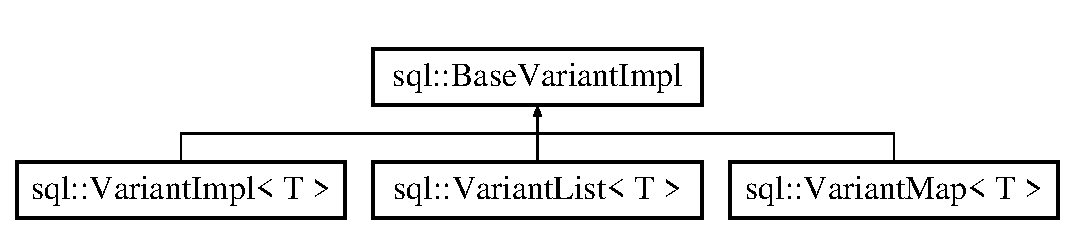
\includegraphics[height=2.000000cm]{classsql_1_1_base_variant_impl}
\end{center}
\end{figure}
\subsection*{Public Member Functions}
\begin{DoxyCompactItemize}
\item 
\hypertarget{classsql_1_1_base_variant_impl_a87a2cb65f36f91d88b83521dd2315b5e}{}\label{classsql_1_1_base_variant_impl_a87a2cb65f36f91d88b83521dd2315b5e} 
{\bfseries Base\+Variant\+Impl} (void $\ast$ptr, \hyperlink{classsql_1_1_s_q_l_string}{sql\+::\+S\+Q\+L\+String} vtype)
\item 
\hypertarget{classsql_1_1_base_variant_impl_a8e53085bd523fe88f18af8ad65ff72fa}{}\label{classsql_1_1_base_variant_impl_a8e53085bd523fe88f18af8ad65ff72fa} 
virtual \hyperlink{classsql_1_1_base_variant_impl}{Base\+Variant\+Impl} $\ast$ {\bfseries Clone} ()=0
\item 
\hypertarget{classsql_1_1_base_variant_impl_a78ccc21b2495cfa8ac7f17a167e88594}{}\label{classsql_1_1_base_variant_impl_a78ccc21b2495cfa8ac7f17a167e88594} 
{\footnotesize template$<$class T $>$ }\\T $\ast$ {\bfseries get} () const
\end{DoxyCompactItemize}
\subsection*{Protected Attributes}
\begin{DoxyCompactItemize}
\item 
\hypertarget{classsql_1_1_base_variant_impl_ab438bc57eece9802274e8c61393b3d73}{}\label{classsql_1_1_base_variant_impl_ab438bc57eece9802274e8c61393b3d73} 
void $\ast$ {\bfseries cvptr}
\item 
\hypertarget{classsql_1_1_base_variant_impl_ae5c0cd2898b6f41624e4c601a3d48810}{}\label{classsql_1_1_base_variant_impl_ae5c0cd2898b6f41624e4c601a3d48810} 
\hyperlink{classsql_1_1_s_q_l_string}{sql\+::\+S\+Q\+L\+String} {\bfseries v\+Type\+Name}
\end{DoxyCompactItemize}


The documentation for this class was generated from the following file\+:\begin{DoxyCompactItemize}
\item 
E\+:/projekt\+\_\+cpp\+\_\+magazyn/projekt/\+Magazyn/\+Magazyn/\+Magazyn/mysql/include/cppconn/variant.\+h\end{DoxyCompactItemize}

\hypertarget{classsql_1_1_connection}{}\section{sql\+:\+:Connection Class Reference}
\label{classsql_1_1_connection}\index{sql\+::\+Connection@{sql\+::\+Connection}}
Inheritance diagram for sql\+:\+:Connection\+:\begin{figure}[H]
\begin{center}
\leavevmode
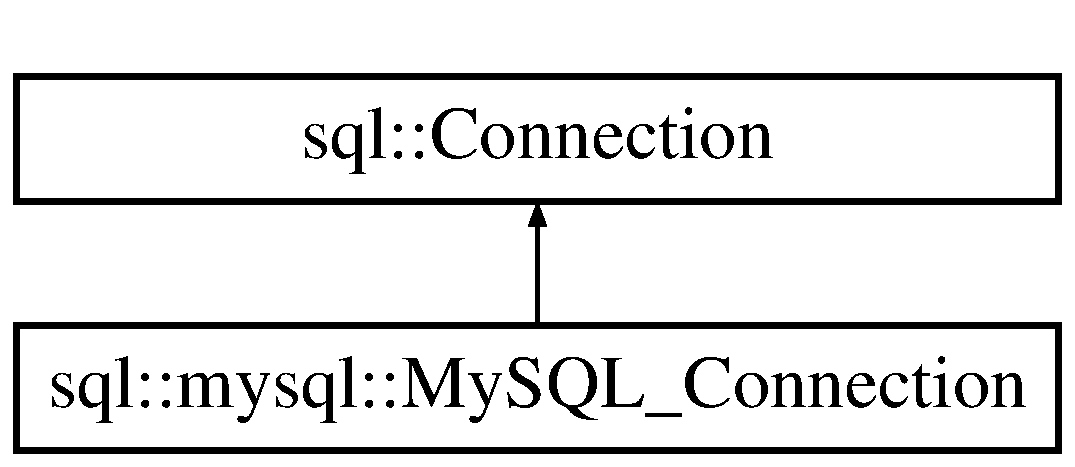
\includegraphics[height=2.000000cm]{classsql_1_1_connection}
\end{center}
\end{figure}
\subsection*{Public Member Functions}
\begin{DoxyCompactItemize}
\item 
\hypertarget{classsql_1_1_connection_adc7b9f8ebed556481f207cb251bfeb06}{}\label{classsql_1_1_connection_adc7b9f8ebed556481f207cb251bfeb06} 
virtual void {\bfseries clear\+Warnings} ()=0
\item 
\hypertarget{classsql_1_1_connection_aa233877114405e5392ea2d2361e0a15c}{}\label{classsql_1_1_connection_aa233877114405e5392ea2d2361e0a15c} 
virtual \hyperlink{classsql_1_1_statement}{Statement} $\ast$ {\bfseries create\+Statement} ()=0
\item 
\hypertarget{classsql_1_1_connection_ad2c949835acad775c52e35f3a4fc5c13}{}\label{classsql_1_1_connection_ad2c949835acad775c52e35f3a4fc5c13} 
virtual void {\bfseries close} ()=0
\item 
\hypertarget{classsql_1_1_connection_a6bea21812167998e6f492f8471e19003}{}\label{classsql_1_1_connection_a6bea21812167998e6f492f8471e19003} 
virtual void {\bfseries commit} ()=0
\item 
\hypertarget{classsql_1_1_connection_a0e5f22278356c25f85e4d3d18f6e2493}{}\label{classsql_1_1_connection_a0e5f22278356c25f85e4d3d18f6e2493} 
virtual bool {\bfseries get\+Auto\+Commit} ()=0
\item 
\hypertarget{classsql_1_1_connection_a55ecebee6958e648bdb2362f80f2e7ea}{}\label{classsql_1_1_connection_a55ecebee6958e648bdb2362f80f2e7ea} 
virtual \hyperlink{classsql_1_1_s_q_l_string}{sql\+::\+S\+Q\+L\+String} {\bfseries get\+Catalog} ()=0
\item 
\hypertarget{classsql_1_1_connection_a7556b7f419baca4d3376382cd1257903}{}\label{classsql_1_1_connection_a7556b7f419baca4d3376382cd1257903} 
virtual \hyperlink{classsql_1_1_driver}{Driver} $\ast$ {\bfseries get\+Driver} ()=0
\item 
\hypertarget{classsql_1_1_connection_a74640969453950f6f616fe3761507609}{}\label{classsql_1_1_connection_a74640969453950f6f616fe3761507609} 
virtual \hyperlink{classsql_1_1_s_q_l_string}{sql\+::\+S\+Q\+L\+String} {\bfseries get\+Schema} ()=0
\item 
\hypertarget{classsql_1_1_connection_a0d4a70af09c4bf98409da46bc2e774d3}{}\label{classsql_1_1_connection_a0d4a70af09c4bf98409da46bc2e774d3} 
virtual \hyperlink{classsql_1_1_s_q_l_string}{sql\+::\+S\+Q\+L\+String} {\bfseries get\+Client\+Info} ()=0
\item 
\hypertarget{classsql_1_1_connection_af229eaaf1cbccba5c5adff81bafc7490}{}\label{classsql_1_1_connection_af229eaaf1cbccba5c5adff81bafc7490} 
virtual void {\bfseries get\+Client\+Option} (const \hyperlink{classsql_1_1_s_q_l_string}{sql\+::\+S\+Q\+L\+String} \&option\+Name, void $\ast$option\+Value)=0
\item 
\hypertarget{classsql_1_1_connection_a8410abb35dd37eafece37963723b8dc9}{}\label{classsql_1_1_connection_a8410abb35dd37eafece37963723b8dc9} 
virtual \hyperlink{classsql_1_1_s_q_l_string}{sql\+::\+S\+Q\+L\+String} {\bfseries get\+Client\+Option} (const \hyperlink{classsql_1_1_s_q_l_string}{sql\+::\+S\+Q\+L\+String} \&option\+Name)=0
\item 
\hypertarget{classsql_1_1_connection_a3c17f434b69575d3bd1be3583cff939a}{}\label{classsql_1_1_connection_a3c17f434b69575d3bd1be3583cff939a} 
virtual \hyperlink{classsql_1_1_database_meta_data}{Database\+Meta\+Data} $\ast$ {\bfseries get\+Meta\+Data} ()=0
\item 
\hypertarget{classsql_1_1_connection_ab52859926b376d2ec4aafe651e4f8e04}{}\label{classsql_1_1_connection_ab52859926b376d2ec4aafe651e4f8e04} 
virtual enum\+\_\+transaction\+\_\+isolation {\bfseries get\+Transaction\+Isolation} ()=0
\item 
\hypertarget{classsql_1_1_connection_a128d3eb822a93a88175ec51ca55380aa}{}\label{classsql_1_1_connection_a128d3eb822a93a88175ec51ca55380aa} 
virtual const \hyperlink{classsql_1_1_s_q_l_warning}{S\+Q\+L\+Warning} $\ast$ {\bfseries get\+Warnings} ()=0
\item 
\hypertarget{classsql_1_1_connection_aef81ff1a57e0fb723287d07706037882}{}\label{classsql_1_1_connection_aef81ff1a57e0fb723287d07706037882} 
virtual bool {\bfseries is\+Closed} ()=0
\item 
\hypertarget{classsql_1_1_connection_a3c0ff46c15fe16f2f18db2621f4b7b15}{}\label{classsql_1_1_connection_a3c0ff46c15fe16f2f18db2621f4b7b15} 
virtual bool {\bfseries is\+Read\+Only} ()=0
\item 
\hypertarget{classsql_1_1_connection_ac5d7d99c0b079b8e787f94181ca08ccb}{}\label{classsql_1_1_connection_ac5d7d99c0b079b8e787f94181ca08ccb} 
virtual bool {\bfseries is\+Valid} ()=0
\item 
\hypertarget{classsql_1_1_connection_af5c9506f3ee5ee20dd56857dbc58eb13}{}\label{classsql_1_1_connection_af5c9506f3ee5ee20dd56857dbc58eb13} 
virtual bool {\bfseries reconnect} ()=0
\item 
\hypertarget{classsql_1_1_connection_a99da5ede96a8c9f2e374a3d6fad8cb51}{}\label{classsql_1_1_connection_a99da5ede96a8c9f2e374a3d6fad8cb51} 
virtual \hyperlink{classsql_1_1_s_q_l_string}{sql\+::\+S\+Q\+L\+String} {\bfseries native\+S\+QL} (const \hyperlink{classsql_1_1_s_q_l_string}{sql\+::\+S\+Q\+L\+String} \&sql)=0
\item 
\hypertarget{classsql_1_1_connection_ad30808d0dffd8cfc6046ed2b688a2d75}{}\label{classsql_1_1_connection_ad30808d0dffd8cfc6046ed2b688a2d75} 
virtual \hyperlink{classsql_1_1_prepared_statement}{Prepared\+Statement} $\ast$ {\bfseries prepare\+Statement} (const \hyperlink{classsql_1_1_s_q_l_string}{sql\+::\+S\+Q\+L\+String} \&sql)=0
\item 
\hypertarget{classsql_1_1_connection_aafe50678f73e87ad3f59e9700f9247cd}{}\label{classsql_1_1_connection_aafe50678f73e87ad3f59e9700f9247cd} 
virtual \hyperlink{classsql_1_1_prepared_statement}{Prepared\+Statement} $\ast$ {\bfseries prepare\+Statement} (const \hyperlink{classsql_1_1_s_q_l_string}{sql\+::\+S\+Q\+L\+String} \&sql, int auto\+Generated\+Keys)=0
\item 
\hypertarget{classsql_1_1_connection_a449be4e4c10b0702d14afa481a63b838}{}\label{classsql_1_1_connection_a449be4e4c10b0702d14afa481a63b838} 
virtual \hyperlink{classsql_1_1_prepared_statement}{Prepared\+Statement} $\ast$ {\bfseries prepare\+Statement} (const \hyperlink{classsql_1_1_s_q_l_string}{sql\+::\+S\+Q\+L\+String} \&sql, int $\ast$column\+Indexes)=0
\item 
\hypertarget{classsql_1_1_connection_aa79514a7f216651ea19698ab2ca9521e}{}\label{classsql_1_1_connection_aa79514a7f216651ea19698ab2ca9521e} 
virtual \hyperlink{classsql_1_1_prepared_statement}{Prepared\+Statement} $\ast$ {\bfseries prepare\+Statement} (const \hyperlink{classsql_1_1_s_q_l_string}{sql\+::\+S\+Q\+L\+String} \&sql, int result\+Set\+Type, int result\+Set\+Concurrency)=0
\item 
\hypertarget{classsql_1_1_connection_a76955dcf34e7bfa21b57a58f468d401a}{}\label{classsql_1_1_connection_a76955dcf34e7bfa21b57a58f468d401a} 
virtual \hyperlink{classsql_1_1_prepared_statement}{Prepared\+Statement} $\ast$ {\bfseries prepare\+Statement} (const \hyperlink{classsql_1_1_s_q_l_string}{sql\+::\+S\+Q\+L\+String} \&sql, int result\+Set\+Type, int result\+Set\+Concurrency, int result\+Set\+Holdability)=0
\item 
\hypertarget{classsql_1_1_connection_a242367d9e97f36cfa8aef7df4ab78c0b}{}\label{classsql_1_1_connection_a242367d9e97f36cfa8aef7df4ab78c0b} 
virtual \hyperlink{classsql_1_1_prepared_statement}{Prepared\+Statement} $\ast$ {\bfseries prepare\+Statement} (const \hyperlink{classsql_1_1_s_q_l_string}{sql\+::\+S\+Q\+L\+String} \&sql, \hyperlink{classsql_1_1_s_q_l_string}{sql\+::\+S\+Q\+L\+String} column\+Names\mbox{[}$\,$\mbox{]})=0
\item 
\hypertarget{classsql_1_1_connection_af63b6bf5ad113035594c5cf2a7e50493}{}\label{classsql_1_1_connection_af63b6bf5ad113035594c5cf2a7e50493} 
virtual void {\bfseries release\+Savepoint} (\hyperlink{classsql_1_1_savepoint}{Savepoint} $\ast$savepoint)=0
\item 
\hypertarget{classsql_1_1_connection_a46e4986f74a1f4055f6dfe4ccbf6b472}{}\label{classsql_1_1_connection_a46e4986f74a1f4055f6dfe4ccbf6b472} 
virtual void {\bfseries rollback} ()=0
\item 
\hypertarget{classsql_1_1_connection_aab86022062e265e1d4a9a7c44c2ca354}{}\label{classsql_1_1_connection_aab86022062e265e1d4a9a7c44c2ca354} 
virtual void {\bfseries rollback} (\hyperlink{classsql_1_1_savepoint}{Savepoint} $\ast$savepoint)=0
\item 
\hypertarget{classsql_1_1_connection_a26fc98c84ea562b77992d0995a2808e5}{}\label{classsql_1_1_connection_a26fc98c84ea562b77992d0995a2808e5} 
virtual void {\bfseries set\+Auto\+Commit} (bool auto\+Commit)=0
\item 
\hypertarget{classsql_1_1_connection_ad0ebcbb493f92eaaaa6eabafc3067b7e}{}\label{classsql_1_1_connection_ad0ebcbb493f92eaaaa6eabafc3067b7e} 
virtual void {\bfseries set\+Catalog} (const \hyperlink{classsql_1_1_s_q_l_string}{sql\+::\+S\+Q\+L\+String} \&catalog)=0
\item 
\hypertarget{classsql_1_1_connection_a5e633c562d8e057c0809d3024ec55788}{}\label{classsql_1_1_connection_a5e633c562d8e057c0809d3024ec55788} 
virtual void {\bfseries set\+Schema} (const \hyperlink{classsql_1_1_s_q_l_string}{sql\+::\+S\+Q\+L\+String} \&catalog)=0
\item 
\hypertarget{classsql_1_1_connection_a971ffff0d1742cb7f9ed76fa2f3b0eb3}{}\label{classsql_1_1_connection_a971ffff0d1742cb7f9ed76fa2f3b0eb3} 
virtual \hyperlink{classsql_1_1_connection}{sql\+::\+Connection} $\ast$ {\bfseries set\+Client\+Option} (const \hyperlink{classsql_1_1_s_q_l_string}{sql\+::\+S\+Q\+L\+String} \&option\+Name, const void $\ast$option\+Value)=0
\item 
\hypertarget{classsql_1_1_connection_ae648a3fa3a755ccd9613d9fbd6980afe}{}\label{classsql_1_1_connection_ae648a3fa3a755ccd9613d9fbd6980afe} 
virtual \hyperlink{classsql_1_1_connection}{sql\+::\+Connection} $\ast$ {\bfseries set\+Client\+Option} (const \hyperlink{classsql_1_1_s_q_l_string}{sql\+::\+S\+Q\+L\+String} \&option\+Name, const \hyperlink{classsql_1_1_s_q_l_string}{sql\+::\+S\+Q\+L\+String} \&option\+Value)=0
\item 
\hypertarget{classsql_1_1_connection_a40ad3e1eb922007b79734e87b5dd428b}{}\label{classsql_1_1_connection_a40ad3e1eb922007b79734e87b5dd428b} 
virtual void {\bfseries set\+Holdability} (int holdability)=0
\item 
\hypertarget{classsql_1_1_connection_aaaa23e9c88ec232e3bcdbbf56e81184e}{}\label{classsql_1_1_connection_aaaa23e9c88ec232e3bcdbbf56e81184e} 
virtual void {\bfseries set\+Read\+Only} (bool read\+Only)=0
\item 
\hypertarget{classsql_1_1_connection_aa9f59b2b67db3783f9669a458e74654b}{}\label{classsql_1_1_connection_aa9f59b2b67db3783f9669a458e74654b} 
virtual \hyperlink{classsql_1_1_savepoint}{Savepoint} $\ast$ {\bfseries set\+Savepoint} ()=0
\item 
\hypertarget{classsql_1_1_connection_ae1b5ee8edc062cb3c510eea6be7d6bdc}{}\label{classsql_1_1_connection_ae1b5ee8edc062cb3c510eea6be7d6bdc} 
virtual \hyperlink{classsql_1_1_savepoint}{Savepoint} $\ast$ {\bfseries set\+Savepoint} (const \hyperlink{classsql_1_1_s_q_l_string}{sql\+::\+S\+Q\+L\+String} \&name)=0
\item 
\hypertarget{classsql_1_1_connection_ac9d4593132f11fc701398c68d4baef5f}{}\label{classsql_1_1_connection_ac9d4593132f11fc701398c68d4baef5f} 
virtual void {\bfseries set\+Transaction\+Isolation} (enum\+\_\+transaction\+\_\+isolation level)=0
\end{DoxyCompactItemize}
\subsection*{Private Member Functions}
\begin{DoxyCompactItemize}
\item 
\hypertarget{classsql_1_1_connection_a0ca42318e5b1a908c53fec07ac33c21a}{}\label{classsql_1_1_connection_a0ca42318e5b1a908c53fec07ac33c21a} 
{\bfseries Connection} (const \hyperlink{classsql_1_1_connection}{Connection} \&)
\item 
\hypertarget{classsql_1_1_connection_a02c6d4b13305ddab8e88a6d426bd7718}{}\label{classsql_1_1_connection_a02c6d4b13305ddab8e88a6d426bd7718} 
void {\bfseries operator=} (\hyperlink{classsql_1_1_connection}{Connection} \&)
\end{DoxyCompactItemize}


The documentation for this class was generated from the following file\+:\begin{DoxyCompactItemize}
\item 
E\+:/projekt\+\_\+cpp\+\_\+magazyn/projekt/\+Magazyn/\+Magazyn/\+Magazyn/mysql/include/cppconn/connection.\+h\end{DoxyCompactItemize}

\hypertarget{classsql_1_1_database_meta_data}{}\section{sql\+:\+:Database\+Meta\+Data Class Reference}
\label{classsql_1_1_database_meta_data}\index{sql\+::\+Database\+Meta\+Data@{sql\+::\+Database\+Meta\+Data}}
\subsection*{Public Types}
\begin{DoxyCompactItemize}
\item 
\hypertarget{classsql_1_1_database_meta_data_a0dc3e909654e4349e96328e05c8ab4ea}{}\label{classsql_1_1_database_meta_data_a0dc3e909654e4349e96328e05c8ab4ea} 
enum \{ {\bfseries attribute\+No\+Nulls} = 0, 
{\bfseries attribute\+Nullable}, 
{\bfseries attribute\+Nullable\+Unknown}
 \}
\item 
\hypertarget{classsql_1_1_database_meta_data_ab6ff2a77908ae0a44576dce6e7fa9bd5}{}\label{classsql_1_1_database_meta_data_ab6ff2a77908ae0a44576dce6e7fa9bd5} 
enum \{ {\bfseries best\+Row\+Temporary} = 0, 
{\bfseries best\+Row\+Transaction}, 
{\bfseries best\+Row\+Session}
 \}
\item 
\hypertarget{classsql_1_1_database_meta_data_a4620f13047275aaf7de6a909ccae16c5}{}\label{classsql_1_1_database_meta_data_a4620f13047275aaf7de6a909ccae16c5} 
enum \{ {\bfseries best\+Row\+Unknown} = 0, 
{\bfseries best\+Row\+Not\+Pseudo}, 
{\bfseries best\+Row\+Pseudo}
 \}
\item 
\hypertarget{classsql_1_1_database_meta_data_a69dd286c919dd6dda0a44cd31c36eac5}{}\label{classsql_1_1_database_meta_data_a69dd286c919dd6dda0a44cd31c36eac5} 
enum \{ {\bfseries column\+No\+Nulls} = 0, 
{\bfseries column\+Nullable}, 
{\bfseries column\+Nullable\+Unknown}
 \}
\item 
\hypertarget{classsql_1_1_database_meta_data_a93220e60b60ae6ccdaffda65ff90988d}{}\label{classsql_1_1_database_meta_data_a93220e60b60ae6ccdaffda65ff90988d} 
enum \{ \newline
{\bfseries imported\+Key\+Cascade} = 0, 
{\bfseries imported\+Key\+Initially\+Deferred}, 
{\bfseries imported\+Key\+Initially\+Immediate}, 
{\bfseries imported\+Key\+No\+Action}, 
\newline
{\bfseries imported\+Key\+Not\+Deferrable}, 
{\bfseries imported\+Key\+Restrict}, 
{\bfseries imported\+Key\+Set\+Default}, 
{\bfseries imported\+Key\+Set\+Null}
 \}
\item 
\hypertarget{classsql_1_1_database_meta_data_a01e82d85f8940a6f7de5f1330ed17516}{}\label{classsql_1_1_database_meta_data_a01e82d85f8940a6f7de5f1330ed17516} 
enum \{ \newline
{\bfseries procedure\+Column\+In} = 0, 
{\bfseries procedure\+Column\+In\+Out}, 
{\bfseries procedure\+Column\+Out}, 
{\bfseries procedure\+Column\+Result}, 
\newline
{\bfseries procedure\+Column\+Return}, 
{\bfseries procedure\+Column\+Unknown}, 
{\bfseries procedure\+No\+Nulls}, 
{\bfseries procedure\+No\+Result}, 
\newline
{\bfseries procedure\+Nullable}, 
{\bfseries procedure\+Nullable\+Unknown}, 
{\bfseries procedure\+Result\+Unknown}, 
{\bfseries procedure\+Returns\+Result}
 \}
\item 
\hypertarget{classsql_1_1_database_meta_data_aad24aedab12fce271e473fdd723bbe86}{}\label{classsql_1_1_database_meta_data_aad24aedab12fce271e473fdd723bbe86} 
enum \{ {\bfseries sql\+State\+S\+Q\+L99} = 0, 
{\bfseries sql\+State\+X\+Open}
 \}
\item 
\hypertarget{classsql_1_1_database_meta_data_a61b9d896dcca26b2297a581e4f952efc}{}\label{classsql_1_1_database_meta_data_a61b9d896dcca26b2297a581e4f952efc} 
enum \{ {\bfseries table\+Index\+Clustered} = 0, 
{\bfseries table\+Index\+Hashed}, 
{\bfseries table\+Index\+Other}, 
{\bfseries table\+Index\+Statistic}
 \}
\item 
\hypertarget{classsql_1_1_database_meta_data_ac1be8c81bf9636c23197cf44ebc03012}{}\label{classsql_1_1_database_meta_data_ac1be8c81bf9636c23197cf44ebc03012} 
enum \{ {\bfseries version\+Column\+Unknown} = 0, 
{\bfseries version\+Column\+Not\+Pseudo} = 1, 
{\bfseries version\+Column\+Pseudo} = 2
 \}
\item 
\hypertarget{classsql_1_1_database_meta_data_a84ba71d4c78795c60e9ae7e391b09b88}{}\label{classsql_1_1_database_meta_data_a84ba71d4c78795c60e9ae7e391b09b88} 
enum \{ {\bfseries type\+No\+Nulls} = 0, 
{\bfseries type\+Nullable} = 1, 
{\bfseries type\+Nullable\+Unknown} = 2
 \}
\item 
\hypertarget{classsql_1_1_database_meta_data_a8201bbaaed4571db1fef210376f87b11}{}\label{classsql_1_1_database_meta_data_a8201bbaaed4571db1fef210376f87b11} 
enum \{ {\bfseries type\+Pred\+None} = 0, 
{\bfseries type\+Pred\+Char} = 1, 
{\bfseries type\+Pred\+Basic} = 2, 
{\bfseries type\+Searchable} = 3
 \}
\end{DoxyCompactItemize}
\subsection*{Public Member Functions}
\begin{DoxyCompactItemize}
\item 
\hypertarget{classsql_1_1_database_meta_data_a0fcfa43f51cbe1bf0d25bae69fbb39ac}{}\label{classsql_1_1_database_meta_data_a0fcfa43f51cbe1bf0d25bae69fbb39ac} 
virtual bool {\bfseries all\+Procedures\+Are\+Callable} ()=0
\item 
\hypertarget{classsql_1_1_database_meta_data_a087fca0afb7cace4db77c16490821acc}{}\label{classsql_1_1_database_meta_data_a087fca0afb7cace4db77c16490821acc} 
virtual bool {\bfseries all\+Tables\+Are\+Selectable} ()=0
\item 
\hypertarget{classsql_1_1_database_meta_data_a8307e470f11b1136fb30b0f85031d2da}{}\label{classsql_1_1_database_meta_data_a8307e470f11b1136fb30b0f85031d2da} 
virtual bool {\bfseries data\+Definition\+Causes\+Transaction\+Commit} ()=0
\item 
\hypertarget{classsql_1_1_database_meta_data_a6d0ab535bca802cba072bb2ac3cb1c95}{}\label{classsql_1_1_database_meta_data_a6d0ab535bca802cba072bb2ac3cb1c95} 
virtual bool {\bfseries data\+Definition\+Ignored\+In\+Transactions} ()=0
\item 
\hypertarget{classsql_1_1_database_meta_data_a0ff634280a6fd1054e7808f8a6da2d0f}{}\label{classsql_1_1_database_meta_data_a0ff634280a6fd1054e7808f8a6da2d0f} 
virtual bool {\bfseries deletes\+Are\+Detected} (int type)=0
\item 
\hypertarget{classsql_1_1_database_meta_data_a5928f3cd90d2880bf49689b5f696e8a2}{}\label{classsql_1_1_database_meta_data_a5928f3cd90d2880bf49689b5f696e8a2} 
virtual bool {\bfseries does\+Max\+Row\+Size\+Include\+Blobs} ()=0
\item 
\hypertarget{classsql_1_1_database_meta_data_a8c95252297cfa93887646dfab1e930ae}{}\label{classsql_1_1_database_meta_data_a8c95252297cfa93887646dfab1e930ae} 
virtual \hyperlink{classsql_1_1_result_set}{Result\+Set} $\ast$ {\bfseries get\+Attributes} (const \hyperlink{classsql_1_1_s_q_l_string}{sql\+::\+S\+Q\+L\+String} \&catalog, const \hyperlink{classsql_1_1_s_q_l_string}{sql\+::\+S\+Q\+L\+String} \&schema\+Pattern, const \hyperlink{classsql_1_1_s_q_l_string}{sql\+::\+S\+Q\+L\+String} \&type\+Name\+Pattern, const \hyperlink{classsql_1_1_s_q_l_string}{sql\+::\+S\+Q\+L\+String} \&attribute\+Name\+Pattern)=0
\item 
\hypertarget{classsql_1_1_database_meta_data_a3914f9fec48b670034357dceedbce42a}{}\label{classsql_1_1_database_meta_data_a3914f9fec48b670034357dceedbce42a} 
virtual \hyperlink{classsql_1_1_result_set}{Result\+Set} $\ast$ {\bfseries get\+Best\+Row\+Identifier} (const \hyperlink{classsql_1_1_s_q_l_string}{sql\+::\+S\+Q\+L\+String} \&catalog, const \hyperlink{classsql_1_1_s_q_l_string}{sql\+::\+S\+Q\+L\+String} \&schema, const \hyperlink{classsql_1_1_s_q_l_string}{sql\+::\+S\+Q\+L\+String} \&table, int scope, bool nullable)=0
\item 
\hypertarget{classsql_1_1_database_meta_data_a5ca54dbc2f5dae656544e77f71312036}{}\label{classsql_1_1_database_meta_data_a5ca54dbc2f5dae656544e77f71312036} 
virtual \hyperlink{classsql_1_1_result_set}{Result\+Set} $\ast$ {\bfseries get\+Catalogs} ()=0
\item 
\hypertarget{classsql_1_1_database_meta_data_a191861504f93a4619c2dc0cffa4b17e7}{}\label{classsql_1_1_database_meta_data_a191861504f93a4619c2dc0cffa4b17e7} 
virtual const \hyperlink{classsql_1_1_s_q_l_string}{sql\+::\+S\+Q\+L\+String} \& {\bfseries get\+Catalog\+Separator} ()=0
\item 
\hypertarget{classsql_1_1_database_meta_data_a8a69bb04c9251af8fc6aa704434f39f1}{}\label{classsql_1_1_database_meta_data_a8a69bb04c9251af8fc6aa704434f39f1} 
virtual const \hyperlink{classsql_1_1_s_q_l_string}{sql\+::\+S\+Q\+L\+String} \& {\bfseries get\+Catalog\+Term} ()=0
\item 
\hypertarget{classsql_1_1_database_meta_data_ae5846ef8fe9f6898d0d5d4c621b6480d}{}\label{classsql_1_1_database_meta_data_ae5846ef8fe9f6898d0d5d4c621b6480d} 
virtual \hyperlink{classsql_1_1_result_set}{Result\+Set} $\ast$ {\bfseries get\+Column\+Privileges} (const \hyperlink{classsql_1_1_s_q_l_string}{sql\+::\+S\+Q\+L\+String} \&catalog, const \hyperlink{classsql_1_1_s_q_l_string}{sql\+::\+S\+Q\+L\+String} \&schema, const \hyperlink{classsql_1_1_s_q_l_string}{sql\+::\+S\+Q\+L\+String} \&table, const \hyperlink{classsql_1_1_s_q_l_string}{sql\+::\+S\+Q\+L\+String} \&column\+Name\+Pattern)=0
\item 
\hypertarget{classsql_1_1_database_meta_data_a6335f2fdd25a724510fdcea2117f8df7}{}\label{classsql_1_1_database_meta_data_a6335f2fdd25a724510fdcea2117f8df7} 
virtual \hyperlink{classsql_1_1_result_set}{Result\+Set} $\ast$ {\bfseries get\+Columns} (const \hyperlink{classsql_1_1_s_q_l_string}{sql\+::\+S\+Q\+L\+String} \&catalog, const \hyperlink{classsql_1_1_s_q_l_string}{sql\+::\+S\+Q\+L\+String} \&schema\+Pattern, const \hyperlink{classsql_1_1_s_q_l_string}{sql\+::\+S\+Q\+L\+String} \&table\+Name\+Pattern, const \hyperlink{classsql_1_1_s_q_l_string}{sql\+::\+S\+Q\+L\+String} \&column\+Name\+Pattern)=0
\item 
\hypertarget{classsql_1_1_database_meta_data_a3a552c4e9a9f1cdea2bde0336cd3806f}{}\label{classsql_1_1_database_meta_data_a3a552c4e9a9f1cdea2bde0336cd3806f} 
virtual \hyperlink{classsql_1_1_connection}{Connection} $\ast$ {\bfseries get\+Connection} ()=0
\item 
\hypertarget{classsql_1_1_database_meta_data_ab570b099e665fd49254f708bd8ba30c8}{}\label{classsql_1_1_database_meta_data_ab570b099e665fd49254f708bd8ba30c8} 
virtual \hyperlink{classsql_1_1_result_set}{Result\+Set} $\ast$ {\bfseries get\+Cross\+Reference} (const \hyperlink{classsql_1_1_s_q_l_string}{sql\+::\+S\+Q\+L\+String} \&primary\+Catalog, const \hyperlink{classsql_1_1_s_q_l_string}{sql\+::\+S\+Q\+L\+String} \&primary\+Schema, const \hyperlink{classsql_1_1_s_q_l_string}{sql\+::\+S\+Q\+L\+String} \&primary\+Table, const \hyperlink{classsql_1_1_s_q_l_string}{sql\+::\+S\+Q\+L\+String} \&foreign\+Catalog, const \hyperlink{classsql_1_1_s_q_l_string}{sql\+::\+S\+Q\+L\+String} \&foreign\+Schema, const \hyperlink{classsql_1_1_s_q_l_string}{sql\+::\+S\+Q\+L\+String} \&foreign\+Table)=0
\item 
\hypertarget{classsql_1_1_database_meta_data_a5833613db9575c1fb36c777787c04c87}{}\label{classsql_1_1_database_meta_data_a5833613db9575c1fb36c777787c04c87} 
virtual unsigned int {\bfseries get\+Database\+Major\+Version} ()=0
\item 
\hypertarget{classsql_1_1_database_meta_data_affe64c548dab5cbcdbc61eb02c3789d9}{}\label{classsql_1_1_database_meta_data_affe64c548dab5cbcdbc61eb02c3789d9} 
virtual unsigned int {\bfseries get\+Database\+Minor\+Version} ()=0
\item 
\hypertarget{classsql_1_1_database_meta_data_aa9b5db63d73ea348c3c911358388a934}{}\label{classsql_1_1_database_meta_data_aa9b5db63d73ea348c3c911358388a934} 
virtual unsigned int {\bfseries get\+Database\+Patch\+Version} ()=0
\item 
\hypertarget{classsql_1_1_database_meta_data_aada5735541b87d374d08b96a97665f68}{}\label{classsql_1_1_database_meta_data_aada5735541b87d374d08b96a97665f68} 
virtual const \hyperlink{classsql_1_1_s_q_l_string}{sql\+::\+S\+Q\+L\+String} \& {\bfseries get\+Database\+Product\+Name} ()=0
\item 
\hypertarget{classsql_1_1_database_meta_data_a3bee431aa9a025dc089e7a43a6c33254}{}\label{classsql_1_1_database_meta_data_a3bee431aa9a025dc089e7a43a6c33254} 
virtual \hyperlink{classsql_1_1_s_q_l_string}{S\+Q\+L\+String} {\bfseries get\+Database\+Product\+Version} ()=0
\item 
\hypertarget{classsql_1_1_database_meta_data_ae9b4fc386b1fcef9bfc0f32770c1d915}{}\label{classsql_1_1_database_meta_data_ae9b4fc386b1fcef9bfc0f32770c1d915} 
virtual int {\bfseries get\+Default\+Transaction\+Isolation} ()=0
\item 
\hypertarget{classsql_1_1_database_meta_data_adf24b72cd1494ea9d0eac347b9d27eeb}{}\label{classsql_1_1_database_meta_data_adf24b72cd1494ea9d0eac347b9d27eeb} 
virtual unsigned int {\bfseries get\+Driver\+Major\+Version} ()=0
\item 
\hypertarget{classsql_1_1_database_meta_data_a0aca6126dccab168a8f80a37ee981572}{}\label{classsql_1_1_database_meta_data_a0aca6126dccab168a8f80a37ee981572} 
virtual unsigned int {\bfseries get\+Driver\+Minor\+Version} ()=0
\item 
\hypertarget{classsql_1_1_database_meta_data_a61bd3f4abd44b3881298d134a5eb3e23}{}\label{classsql_1_1_database_meta_data_a61bd3f4abd44b3881298d134a5eb3e23} 
virtual unsigned int {\bfseries get\+Driver\+Patch\+Version} ()=0
\item 
\hypertarget{classsql_1_1_database_meta_data_af4ca8e69a8eeb1d8c1e8e7ddf9c4275b}{}\label{classsql_1_1_database_meta_data_af4ca8e69a8eeb1d8c1e8e7ddf9c4275b} 
virtual const \hyperlink{classsql_1_1_s_q_l_string}{sql\+::\+S\+Q\+L\+String} \& {\bfseries get\+Driver\+Name} ()=0
\item 
\hypertarget{classsql_1_1_database_meta_data_a62c128d6c9518f3d4d72cb428b08f915}{}\label{classsql_1_1_database_meta_data_a62c128d6c9518f3d4d72cb428b08f915} 
virtual const \hyperlink{classsql_1_1_s_q_l_string}{sql\+::\+S\+Q\+L\+String} \& {\bfseries get\+Driver\+Version} ()=0
\item 
\hypertarget{classsql_1_1_database_meta_data_aa3c0a69a0cdaf26d9aec3e8e9353660b}{}\label{classsql_1_1_database_meta_data_aa3c0a69a0cdaf26d9aec3e8e9353660b} 
virtual \hyperlink{classsql_1_1_result_set}{Result\+Set} $\ast$ {\bfseries get\+Exported\+Keys} (const \hyperlink{classsql_1_1_s_q_l_string}{sql\+::\+S\+Q\+L\+String} \&catalog, const \hyperlink{classsql_1_1_s_q_l_string}{sql\+::\+S\+Q\+L\+String} \&schema, const \hyperlink{classsql_1_1_s_q_l_string}{sql\+::\+S\+Q\+L\+String} \&table)=0
\item 
\hypertarget{classsql_1_1_database_meta_data_ad69fbdc5f394fdcc273478918733d773}{}\label{classsql_1_1_database_meta_data_ad69fbdc5f394fdcc273478918733d773} 
virtual const \hyperlink{classsql_1_1_s_q_l_string}{sql\+::\+S\+Q\+L\+String} \& {\bfseries get\+Extra\+Name\+Characters} ()=0
\item 
\hypertarget{classsql_1_1_database_meta_data_af7346d0eb62559c73c3f10610b662b29}{}\label{classsql_1_1_database_meta_data_af7346d0eb62559c73c3f10610b662b29} 
virtual const \hyperlink{classsql_1_1_s_q_l_string}{sql\+::\+S\+Q\+L\+String} \& {\bfseries get\+Identifier\+Quote\+String} ()=0
\item 
\hypertarget{classsql_1_1_database_meta_data_a3ac26171c59a06c53208a63168b4cf61}{}\label{classsql_1_1_database_meta_data_a3ac26171c59a06c53208a63168b4cf61} 
virtual \hyperlink{classsql_1_1_result_set}{Result\+Set} $\ast$ {\bfseries get\+Imported\+Keys} (const \hyperlink{classsql_1_1_s_q_l_string}{sql\+::\+S\+Q\+L\+String} \&catalog, const \hyperlink{classsql_1_1_s_q_l_string}{sql\+::\+S\+Q\+L\+String} \&schema, const \hyperlink{classsql_1_1_s_q_l_string}{sql\+::\+S\+Q\+L\+String} \&table)=0
\item 
\hypertarget{classsql_1_1_database_meta_data_a09f632ada5648652bf48d2a2b6896a82}{}\label{classsql_1_1_database_meta_data_a09f632ada5648652bf48d2a2b6896a82} 
virtual \hyperlink{classsql_1_1_result_set}{Result\+Set} $\ast$ {\bfseries get\+Index\+Info} (const \hyperlink{classsql_1_1_s_q_l_string}{sql\+::\+S\+Q\+L\+String} \&catalog, const \hyperlink{classsql_1_1_s_q_l_string}{sql\+::\+S\+Q\+L\+String} \&schema, const \hyperlink{classsql_1_1_s_q_l_string}{sql\+::\+S\+Q\+L\+String} \&table, bool unique, bool approximate)=0
\item 
\hypertarget{classsql_1_1_database_meta_data_a6e6846d4a1438825ceffb9f18293260a}{}\label{classsql_1_1_database_meta_data_a6e6846d4a1438825ceffb9f18293260a} 
virtual unsigned int {\bfseries get\+C\+D\+B\+C\+Major\+Version} ()=0
\item 
\hypertarget{classsql_1_1_database_meta_data_a16a975c983b124f831ec843cb50b1932}{}\label{classsql_1_1_database_meta_data_a16a975c983b124f831ec843cb50b1932} 
virtual unsigned int {\bfseries get\+C\+D\+B\+C\+Minor\+Version} ()=0
\item 
\hypertarget{classsql_1_1_database_meta_data_a397f14bc6f3b2194b0eec3e23d205bea}{}\label{classsql_1_1_database_meta_data_a397f14bc6f3b2194b0eec3e23d205bea} 
virtual unsigned int {\bfseries get\+Max\+Binary\+Literal\+Length} ()=0
\item 
\hypertarget{classsql_1_1_database_meta_data_a44cda683cedda5a2ce0bc94b93b39803}{}\label{classsql_1_1_database_meta_data_a44cda683cedda5a2ce0bc94b93b39803} 
virtual unsigned int {\bfseries get\+Max\+Catalog\+Name\+Length} ()=0
\item 
\hypertarget{classsql_1_1_database_meta_data_a82ff0807ddf8c7cf18043b12831d3af1}{}\label{classsql_1_1_database_meta_data_a82ff0807ddf8c7cf18043b12831d3af1} 
virtual unsigned int {\bfseries get\+Max\+Char\+Literal\+Length} ()=0
\item 
\hypertarget{classsql_1_1_database_meta_data_abac3fba335d07e951ef4b3ca9e8ece54}{}\label{classsql_1_1_database_meta_data_abac3fba335d07e951ef4b3ca9e8ece54} 
virtual unsigned int {\bfseries get\+Max\+Column\+Name\+Length} ()=0
\item 
\hypertarget{classsql_1_1_database_meta_data_adbfe2f668577edb968a0fc1437b322df}{}\label{classsql_1_1_database_meta_data_adbfe2f668577edb968a0fc1437b322df} 
virtual unsigned int {\bfseries get\+Max\+Columns\+In\+Group\+By} ()=0
\item 
\hypertarget{classsql_1_1_database_meta_data_a4e797622f6accf276b8b2e4bdf6e1fe6}{}\label{classsql_1_1_database_meta_data_a4e797622f6accf276b8b2e4bdf6e1fe6} 
virtual unsigned int {\bfseries get\+Max\+Columns\+In\+Index} ()=0
\item 
\hypertarget{classsql_1_1_database_meta_data_affe2aa7ee1752d02ad509bb83b48b414}{}\label{classsql_1_1_database_meta_data_affe2aa7ee1752d02ad509bb83b48b414} 
virtual unsigned int {\bfseries get\+Max\+Columns\+In\+Order\+By} ()=0
\item 
\hypertarget{classsql_1_1_database_meta_data_a172e91cb97d54c28ab41ceb919ecccd9}{}\label{classsql_1_1_database_meta_data_a172e91cb97d54c28ab41ceb919ecccd9} 
virtual unsigned int {\bfseries get\+Max\+Columns\+In\+Select} ()=0
\item 
\hypertarget{classsql_1_1_database_meta_data_a6a9ebc216dc3ef347461324f80dd76a6}{}\label{classsql_1_1_database_meta_data_a6a9ebc216dc3ef347461324f80dd76a6} 
virtual unsigned int {\bfseries get\+Max\+Columns\+In\+Table} ()=0
\item 
\hypertarget{classsql_1_1_database_meta_data_a636a1d77f36dca5db32c8fb4138b31d0}{}\label{classsql_1_1_database_meta_data_a636a1d77f36dca5db32c8fb4138b31d0} 
virtual unsigned int {\bfseries get\+Max\+Connections} ()=0
\item 
\hypertarget{classsql_1_1_database_meta_data_aff35039d257d98d53b8dc57cb89c734d}{}\label{classsql_1_1_database_meta_data_aff35039d257d98d53b8dc57cb89c734d} 
virtual unsigned int {\bfseries get\+Max\+Cursor\+Name\+Length} ()=0
\item 
\hypertarget{classsql_1_1_database_meta_data_ab2d270d2248a05a9730966a60538d4e8}{}\label{classsql_1_1_database_meta_data_ab2d270d2248a05a9730966a60538d4e8} 
virtual unsigned int {\bfseries get\+Max\+Index\+Length} ()=0
\item 
\hypertarget{classsql_1_1_database_meta_data_a198de22c6dc79910e334c636ef436d4f}{}\label{classsql_1_1_database_meta_data_a198de22c6dc79910e334c636ef436d4f} 
virtual unsigned int {\bfseries get\+Max\+Procedure\+Name\+Length} ()=0
\item 
\hypertarget{classsql_1_1_database_meta_data_ad3969ced5c3588235ea1b1d0abb2f54e}{}\label{classsql_1_1_database_meta_data_ad3969ced5c3588235ea1b1d0abb2f54e} 
virtual unsigned int {\bfseries get\+Max\+Row\+Size} ()=0
\item 
\hypertarget{classsql_1_1_database_meta_data_a6402d54f7ab4aab9fb6a0fb0f4f789f9}{}\label{classsql_1_1_database_meta_data_a6402d54f7ab4aab9fb6a0fb0f4f789f9} 
virtual unsigned int {\bfseries get\+Max\+Schema\+Name\+Length} ()=0
\item 
\hypertarget{classsql_1_1_database_meta_data_a03e2eeff7cb8ba131f883001ebfc28e4}{}\label{classsql_1_1_database_meta_data_a03e2eeff7cb8ba131f883001ebfc28e4} 
virtual unsigned int {\bfseries get\+Max\+Statement\+Length} ()=0
\item 
\hypertarget{classsql_1_1_database_meta_data_ac70729ade189e82f16d14ab816eb0c68}{}\label{classsql_1_1_database_meta_data_ac70729ade189e82f16d14ab816eb0c68} 
virtual unsigned int {\bfseries get\+Max\+Statements} ()=0
\item 
\hypertarget{classsql_1_1_database_meta_data_a0de009aca4a8c89a424e04c84598f5c1}{}\label{classsql_1_1_database_meta_data_a0de009aca4a8c89a424e04c84598f5c1} 
virtual unsigned int {\bfseries get\+Max\+Table\+Name\+Length} ()=0
\item 
\hypertarget{classsql_1_1_database_meta_data_a3b0131ea0ae4bb88c484555b4b02a305}{}\label{classsql_1_1_database_meta_data_a3b0131ea0ae4bb88c484555b4b02a305} 
virtual unsigned int {\bfseries get\+Max\+Tables\+In\+Select} ()=0
\item 
\hypertarget{classsql_1_1_database_meta_data_ac53ea52db09abf98b0ef4334a5854ff1}{}\label{classsql_1_1_database_meta_data_ac53ea52db09abf98b0ef4334a5854ff1} 
virtual unsigned int {\bfseries get\+Max\+User\+Name\+Length} ()=0
\item 
\hypertarget{classsql_1_1_database_meta_data_a14b53a06afac6626f0b1bfce43109df7}{}\label{classsql_1_1_database_meta_data_a14b53a06afac6626f0b1bfce43109df7} 
virtual const \hyperlink{classsql_1_1_s_q_l_string}{sql\+::\+S\+Q\+L\+String} \& {\bfseries get\+Numeric\+Functions} ()=0
\item 
\hypertarget{classsql_1_1_database_meta_data_add967db3b1fe2defafbdbc26bf3bd35a}{}\label{classsql_1_1_database_meta_data_add967db3b1fe2defafbdbc26bf3bd35a} 
virtual \hyperlink{classsql_1_1_result_set}{Result\+Set} $\ast$ {\bfseries get\+Primary\+Keys} (const \hyperlink{classsql_1_1_s_q_l_string}{sql\+::\+S\+Q\+L\+String} \&catalog, const \hyperlink{classsql_1_1_s_q_l_string}{sql\+::\+S\+Q\+L\+String} \&schema, const \hyperlink{classsql_1_1_s_q_l_string}{sql\+::\+S\+Q\+L\+String} \&table)=0
\item 
\hypertarget{classsql_1_1_database_meta_data_acc5d42453f7ab2e1314b97e29051cd2e}{}\label{classsql_1_1_database_meta_data_acc5d42453f7ab2e1314b97e29051cd2e} 
virtual \hyperlink{classsql_1_1_result_set}{Result\+Set} $\ast$ {\bfseries get\+Procedure\+Columns} (const \hyperlink{classsql_1_1_s_q_l_string}{sql\+::\+S\+Q\+L\+String} \&catalog, const \hyperlink{classsql_1_1_s_q_l_string}{sql\+::\+S\+Q\+L\+String} \&schema\+Pattern, const \hyperlink{classsql_1_1_s_q_l_string}{sql\+::\+S\+Q\+L\+String} \&procedure\+Name\+Pattern, const \hyperlink{classsql_1_1_s_q_l_string}{sql\+::\+S\+Q\+L\+String} \&column\+Name\+Pattern)=0
\item 
\hypertarget{classsql_1_1_database_meta_data_ac27e60d74934641fe7fcbefae4842835}{}\label{classsql_1_1_database_meta_data_ac27e60d74934641fe7fcbefae4842835} 
virtual \hyperlink{classsql_1_1_result_set}{Result\+Set} $\ast$ {\bfseries get\+Procedures} (const \hyperlink{classsql_1_1_s_q_l_string}{sql\+::\+S\+Q\+L\+String} \&catalog, const \hyperlink{classsql_1_1_s_q_l_string}{sql\+::\+S\+Q\+L\+String} \&schema\+Pattern, const \hyperlink{classsql_1_1_s_q_l_string}{sql\+::\+S\+Q\+L\+String} \&procedure\+Name\+Pattern)=0
\item 
\hypertarget{classsql_1_1_database_meta_data_a64ffac3e5ce785a9f530b6debf79e8dc}{}\label{classsql_1_1_database_meta_data_a64ffac3e5ce785a9f530b6debf79e8dc} 
virtual const \hyperlink{classsql_1_1_s_q_l_string}{sql\+::\+S\+Q\+L\+String} \& {\bfseries get\+Procedure\+Term} ()=0
\item 
\hypertarget{classsql_1_1_database_meta_data_aa99ad098ea64c9aaf216688bc9bbe2b7}{}\label{classsql_1_1_database_meta_data_aa99ad098ea64c9aaf216688bc9bbe2b7} 
virtual int {\bfseries get\+Result\+Set\+Holdability} ()=0
\item 
\hypertarget{classsql_1_1_database_meta_data_aa84ae70b639eb3584b7fa110b4cb4e11}{}\label{classsql_1_1_database_meta_data_aa84ae70b639eb3584b7fa110b4cb4e11} 
virtual \hyperlink{classsql_1_1_result_set}{Result\+Set} $\ast$ {\bfseries get\+Schemas} ()=0
\item 
\hypertarget{classsql_1_1_database_meta_data_ae84cd0fe174b1ee8c10c3088772f0a43}{}\label{classsql_1_1_database_meta_data_ae84cd0fe174b1ee8c10c3088772f0a43} 
virtual const \hyperlink{classsql_1_1_s_q_l_string}{sql\+::\+S\+Q\+L\+String} \& {\bfseries get\+Schema\+Term} ()=0
\item 
\hypertarget{classsql_1_1_database_meta_data_a1db2eebd3ecf4afeab01f8c4079d9e6d}{}\label{classsql_1_1_database_meta_data_a1db2eebd3ecf4afeab01f8c4079d9e6d} 
virtual \hyperlink{classsql_1_1_result_set}{Result\+Set} $\ast$ {\bfseries get\+Schema\+Collation} (const \hyperlink{classsql_1_1_s_q_l_string}{sql\+::\+S\+Q\+L\+String} \&catalog, const \hyperlink{classsql_1_1_s_q_l_string}{sql\+::\+S\+Q\+L\+String} \&schema\+Pattern)=0
\item 
\hypertarget{classsql_1_1_database_meta_data_a0c964a17b067027d7bc09404044df70b}{}\label{classsql_1_1_database_meta_data_a0c964a17b067027d7bc09404044df70b} 
virtual \hyperlink{classsql_1_1_result_set}{Result\+Set} $\ast$ {\bfseries get\+Schema\+Charset} (const \hyperlink{classsql_1_1_s_q_l_string}{sql\+::\+S\+Q\+L\+String} \&catalog, const \hyperlink{classsql_1_1_s_q_l_string}{sql\+::\+S\+Q\+L\+String} \&schema\+Pattern)=0
\item 
\hypertarget{classsql_1_1_database_meta_data_a217547c050e085b3acf1ba9c6e90781a}{}\label{classsql_1_1_database_meta_data_a217547c050e085b3acf1ba9c6e90781a} 
virtual const \hyperlink{classsql_1_1_s_q_l_string}{sql\+::\+S\+Q\+L\+String} \& {\bfseries get\+Search\+String\+Escape} ()=0
\item 
\hypertarget{classsql_1_1_database_meta_data_a36233c7037dc74685e328caaa871adbe}{}\label{classsql_1_1_database_meta_data_a36233c7037dc74685e328caaa871adbe} 
virtual const \hyperlink{classsql_1_1_s_q_l_string}{sql\+::\+S\+Q\+L\+String} \& {\bfseries get\+S\+Q\+L\+Keywords} ()=0
\item 
\hypertarget{classsql_1_1_database_meta_data_ac8b7d169651ffebd35eabaae3291af98}{}\label{classsql_1_1_database_meta_data_ac8b7d169651ffebd35eabaae3291af98} 
virtual int {\bfseries get\+S\+Q\+L\+State\+Type} ()=0
\item 
\hypertarget{classsql_1_1_database_meta_data_a7557b51ae3bad4909a00c84ab23cc8f0}{}\label{classsql_1_1_database_meta_data_a7557b51ae3bad4909a00c84ab23cc8f0} 
virtual const \hyperlink{classsql_1_1_s_q_l_string}{sql\+::\+S\+Q\+L\+String} \& {\bfseries get\+String\+Functions} ()=0
\item 
\hypertarget{classsql_1_1_database_meta_data_a8fdb620034349c10b330b891361d5d3e}{}\label{classsql_1_1_database_meta_data_a8fdb620034349c10b330b891361d5d3e} 
virtual \hyperlink{classsql_1_1_result_set}{Result\+Set} $\ast$ {\bfseries get\+Super\+Tables} (const \hyperlink{classsql_1_1_s_q_l_string}{sql\+::\+S\+Q\+L\+String} \&catalog, const \hyperlink{classsql_1_1_s_q_l_string}{sql\+::\+S\+Q\+L\+String} \&schema\+Pattern, const \hyperlink{classsql_1_1_s_q_l_string}{sql\+::\+S\+Q\+L\+String} \&table\+Name\+Pattern)=0
\item 
\hypertarget{classsql_1_1_database_meta_data_aeb74890167a860e207a0babe0c5414c0}{}\label{classsql_1_1_database_meta_data_aeb74890167a860e207a0babe0c5414c0} 
virtual \hyperlink{classsql_1_1_result_set}{Result\+Set} $\ast$ {\bfseries get\+Super\+Types} (const \hyperlink{classsql_1_1_s_q_l_string}{sql\+::\+S\+Q\+L\+String} \&catalog, const \hyperlink{classsql_1_1_s_q_l_string}{sql\+::\+S\+Q\+L\+String} \&schema\+Pattern, const \hyperlink{classsql_1_1_s_q_l_string}{sql\+::\+S\+Q\+L\+String} \&type\+Name\+Pattern)=0
\item 
\hypertarget{classsql_1_1_database_meta_data_af1d38d4907354e79b65dff8f39b6b58c}{}\label{classsql_1_1_database_meta_data_af1d38d4907354e79b65dff8f39b6b58c} 
virtual const \hyperlink{classsql_1_1_s_q_l_string}{sql\+::\+S\+Q\+L\+String} \& {\bfseries get\+System\+Functions} ()=0
\item 
\hypertarget{classsql_1_1_database_meta_data_af79b09cf6116f630f2040d9f5e328ede}{}\label{classsql_1_1_database_meta_data_af79b09cf6116f630f2040d9f5e328ede} 
virtual \hyperlink{classsql_1_1_result_set}{Result\+Set} $\ast$ {\bfseries get\+Table\+Privileges} (const \hyperlink{classsql_1_1_s_q_l_string}{sql\+::\+S\+Q\+L\+String} \&catalog, const \hyperlink{classsql_1_1_s_q_l_string}{sql\+::\+S\+Q\+L\+String} \&schema\+Pattern, const \hyperlink{classsql_1_1_s_q_l_string}{sql\+::\+S\+Q\+L\+String} \&table\+Name\+Pattern)=0
\item 
\hypertarget{classsql_1_1_database_meta_data_a4f5e31c5487e52d4d8cac5834b8b717e}{}\label{classsql_1_1_database_meta_data_a4f5e31c5487e52d4d8cac5834b8b717e} 
virtual \hyperlink{classsql_1_1_result_set}{Result\+Set} $\ast$ {\bfseries get\+Tables} (const \hyperlink{classsql_1_1_s_q_l_string}{sql\+::\+S\+Q\+L\+String} \&catalog, const \hyperlink{classsql_1_1_s_q_l_string}{sql\+::\+S\+Q\+L\+String} \&schema\+Pattern, const \hyperlink{classsql_1_1_s_q_l_string}{sql\+::\+S\+Q\+L\+String} \&table\+Name\+Pattern, std\+::list$<$ \hyperlink{classsql_1_1_s_q_l_string}{sql\+::\+S\+Q\+L\+String} $>$ \&types)=0
\item 
\hypertarget{classsql_1_1_database_meta_data_ac131128f2863420bba3bcb75ee4f76e1}{}\label{classsql_1_1_database_meta_data_ac131128f2863420bba3bcb75ee4f76e1} 
virtual \hyperlink{classsql_1_1_result_set}{Result\+Set} $\ast$ {\bfseries get\+Table\+Types} ()=0
\item 
\hypertarget{classsql_1_1_database_meta_data_ac9a86a8540d7f314a5f83b6a06e610d9}{}\label{classsql_1_1_database_meta_data_ac9a86a8540d7f314a5f83b6a06e610d9} 
virtual \hyperlink{classsql_1_1_result_set}{Result\+Set} $\ast$ {\bfseries get\+Table\+Collation} (const \hyperlink{classsql_1_1_s_q_l_string}{sql\+::\+S\+Q\+L\+String} \&catalog, const \hyperlink{classsql_1_1_s_q_l_string}{sql\+::\+S\+Q\+L\+String} \&schema\+Pattern, const \hyperlink{classsql_1_1_s_q_l_string}{sql\+::\+S\+Q\+L\+String} \&table\+Name\+Pattern)=0
\item 
\hypertarget{classsql_1_1_database_meta_data_aec136e1a062d248cb1c306965b2c70cf}{}\label{classsql_1_1_database_meta_data_aec136e1a062d248cb1c306965b2c70cf} 
virtual \hyperlink{classsql_1_1_result_set}{Result\+Set} $\ast$ {\bfseries get\+Table\+Charset} (const \hyperlink{classsql_1_1_s_q_l_string}{sql\+::\+S\+Q\+L\+String} \&catalog, const \hyperlink{classsql_1_1_s_q_l_string}{sql\+::\+S\+Q\+L\+String} \&schema\+Pattern, const \hyperlink{classsql_1_1_s_q_l_string}{sql\+::\+S\+Q\+L\+String} \&table\+Name\+Pattern)=0
\item 
\hypertarget{classsql_1_1_database_meta_data_ace7a16a15c96196290fa85198a00cfdb}{}\label{classsql_1_1_database_meta_data_ace7a16a15c96196290fa85198a00cfdb} 
virtual const \hyperlink{classsql_1_1_s_q_l_string}{sql\+::\+S\+Q\+L\+String} \& {\bfseries get\+Time\+Date\+Functions} ()=0
\item 
\hypertarget{classsql_1_1_database_meta_data_acf8340fcb22c308f2f1a7cb65519562a}{}\label{classsql_1_1_database_meta_data_acf8340fcb22c308f2f1a7cb65519562a} 
virtual \hyperlink{classsql_1_1_result_set}{Result\+Set} $\ast$ {\bfseries get\+Type\+Info} ()=0
\item 
\hypertarget{classsql_1_1_database_meta_data_a35017d040f6af3cf706f7a7ba5d11998}{}\label{classsql_1_1_database_meta_data_a35017d040f6af3cf706f7a7ba5d11998} 
virtual \hyperlink{classsql_1_1_result_set}{Result\+Set} $\ast$ {\bfseries get\+U\+D\+Ts} (const \hyperlink{classsql_1_1_s_q_l_string}{sql\+::\+S\+Q\+L\+String} \&catalog, const \hyperlink{classsql_1_1_s_q_l_string}{sql\+::\+S\+Q\+L\+String} \&schema\+Pattern, const \hyperlink{classsql_1_1_s_q_l_string}{sql\+::\+S\+Q\+L\+String} \&type\+Name\+Pattern, std\+::list$<$ int $>$ \&types)=0
\item 
\hypertarget{classsql_1_1_database_meta_data_a90b95eca91e938bd6242a7b93c217633}{}\label{classsql_1_1_database_meta_data_a90b95eca91e938bd6242a7b93c217633} 
virtual \hyperlink{classsql_1_1_s_q_l_string}{S\+Q\+L\+String} {\bfseries get\+U\+RL} ()=0
\item 
\hypertarget{classsql_1_1_database_meta_data_a9fe385fcc9618981b70cd5f2ae4163ba}{}\label{classsql_1_1_database_meta_data_a9fe385fcc9618981b70cd5f2ae4163ba} 
virtual \hyperlink{classsql_1_1_s_q_l_string}{S\+Q\+L\+String} {\bfseries get\+User\+Name} ()=0
\item 
\hypertarget{classsql_1_1_database_meta_data_a0217b3964e564039c9e616ace17ed9fa}{}\label{classsql_1_1_database_meta_data_a0217b3964e564039c9e616ace17ed9fa} 
virtual \hyperlink{classsql_1_1_result_set}{Result\+Set} $\ast$ {\bfseries get\+Version\+Columns} (const \hyperlink{classsql_1_1_s_q_l_string}{sql\+::\+S\+Q\+L\+String} \&catalog, const \hyperlink{classsql_1_1_s_q_l_string}{sql\+::\+S\+Q\+L\+String} \&schema, const \hyperlink{classsql_1_1_s_q_l_string}{sql\+::\+S\+Q\+L\+String} \&table)=0
\item 
\hypertarget{classsql_1_1_database_meta_data_a21d652b192599e0574361b0acdb1def8}{}\label{classsql_1_1_database_meta_data_a21d652b192599e0574361b0acdb1def8} 
virtual bool {\bfseries inserts\+Are\+Detected} (int type)=0
\item 
\hypertarget{classsql_1_1_database_meta_data_a883835fd1bab9b119c4f597e56828687}{}\label{classsql_1_1_database_meta_data_a883835fd1bab9b119c4f597e56828687} 
virtual bool {\bfseries is\+Catalog\+At\+Start} ()=0
\item 
\hypertarget{classsql_1_1_database_meta_data_a3b49f4c71b9589c73d1c73fc05ccedea}{}\label{classsql_1_1_database_meta_data_a3b49f4c71b9589c73d1c73fc05ccedea} 
virtual bool {\bfseries is\+Read\+Only} ()=0
\item 
\hypertarget{classsql_1_1_database_meta_data_a3d99b0398c99d00af3ee7866e24b5287}{}\label{classsql_1_1_database_meta_data_a3d99b0398c99d00af3ee7866e24b5287} 
virtual bool {\bfseries locators\+Update\+Copy} ()=0
\item 
\hypertarget{classsql_1_1_database_meta_data_a92cce4e529c70dc4108da4a862fbc813}{}\label{classsql_1_1_database_meta_data_a92cce4e529c70dc4108da4a862fbc813} 
virtual bool {\bfseries null\+Plus\+Non\+Null\+Is\+Null} ()=0
\item 
\hypertarget{classsql_1_1_database_meta_data_a9eddeb9a9624aaf08add52b25fed99e2}{}\label{classsql_1_1_database_meta_data_a9eddeb9a9624aaf08add52b25fed99e2} 
virtual bool {\bfseries nulls\+Are\+Sorted\+At\+End} ()=0
\item 
\hypertarget{classsql_1_1_database_meta_data_a14804cc7855e536d06e6e4e958638745}{}\label{classsql_1_1_database_meta_data_a14804cc7855e536d06e6e4e958638745} 
virtual bool {\bfseries nulls\+Are\+Sorted\+At\+Start} ()=0
\item 
\hypertarget{classsql_1_1_database_meta_data_a71e0e231ef14252538014a37779b1bef}{}\label{classsql_1_1_database_meta_data_a71e0e231ef14252538014a37779b1bef} 
virtual bool {\bfseries nulls\+Are\+Sorted\+High} ()=0
\item 
\hypertarget{classsql_1_1_database_meta_data_a4043cd2e87dff21d4a235115bddfa675}{}\label{classsql_1_1_database_meta_data_a4043cd2e87dff21d4a235115bddfa675} 
virtual bool {\bfseries nulls\+Are\+Sorted\+Low} ()=0
\item 
\hypertarget{classsql_1_1_database_meta_data_a718aadd6d991022955fcf709a7015b01}{}\label{classsql_1_1_database_meta_data_a718aadd6d991022955fcf709a7015b01} 
virtual bool {\bfseries others\+Deletes\+Are\+Visible} (int type)=0
\item 
\hypertarget{classsql_1_1_database_meta_data_a66e81bddf81337cec0f369bad21f1f3a}{}\label{classsql_1_1_database_meta_data_a66e81bddf81337cec0f369bad21f1f3a} 
virtual bool {\bfseries others\+Inserts\+Are\+Visible} (int type)=0
\item 
\hypertarget{classsql_1_1_database_meta_data_ae90d5439f0ad75666318a9a996c9491d}{}\label{classsql_1_1_database_meta_data_ae90d5439f0ad75666318a9a996c9491d} 
virtual bool {\bfseries others\+Updates\+Are\+Visible} (int type)=0
\item 
\hypertarget{classsql_1_1_database_meta_data_a269fab010a5d2b309e7bbdc13f0702c8}{}\label{classsql_1_1_database_meta_data_a269fab010a5d2b309e7bbdc13f0702c8} 
virtual bool {\bfseries own\+Deletes\+Are\+Visible} (int type)=0
\item 
\hypertarget{classsql_1_1_database_meta_data_ae703402e31eeca2a7befaec316447c0c}{}\label{classsql_1_1_database_meta_data_ae703402e31eeca2a7befaec316447c0c} 
virtual bool {\bfseries own\+Inserts\+Are\+Visible} (int type)=0
\item 
\hypertarget{classsql_1_1_database_meta_data_a6f7a7ef19729070d56949266a8071acb}{}\label{classsql_1_1_database_meta_data_a6f7a7ef19729070d56949266a8071acb} 
virtual bool {\bfseries own\+Updates\+Are\+Visible} (int type)=0
\item 
\hypertarget{classsql_1_1_database_meta_data_a124ce82691fef8f4818686d96dca1d11}{}\label{classsql_1_1_database_meta_data_a124ce82691fef8f4818686d96dca1d11} 
virtual bool {\bfseries stores\+Lower\+Case\+Identifiers} ()=0
\item 
\hypertarget{classsql_1_1_database_meta_data_ae3b3c87912943b27c2944645e69dfb1a}{}\label{classsql_1_1_database_meta_data_ae3b3c87912943b27c2944645e69dfb1a} 
virtual bool {\bfseries stores\+Lower\+Case\+Quoted\+Identifiers} ()=0
\item 
\hypertarget{classsql_1_1_database_meta_data_ac3201371230616a24eae3bc48e908c6a}{}\label{classsql_1_1_database_meta_data_ac3201371230616a24eae3bc48e908c6a} 
virtual bool {\bfseries stores\+Mixed\+Case\+Identifiers} ()=0
\item 
\hypertarget{classsql_1_1_database_meta_data_a8681a718baac0dd170e708d785148ffa}{}\label{classsql_1_1_database_meta_data_a8681a718baac0dd170e708d785148ffa} 
virtual bool {\bfseries stores\+Mixed\+Case\+Quoted\+Identifiers} ()=0
\item 
\hypertarget{classsql_1_1_database_meta_data_aca12603a6c30703aebc4f85367f5d00b}{}\label{classsql_1_1_database_meta_data_aca12603a6c30703aebc4f85367f5d00b} 
virtual bool {\bfseries stores\+Upper\+Case\+Identifiers} ()=0
\item 
\hypertarget{classsql_1_1_database_meta_data_ae3084c4785756d127b79b3f55a040d83}{}\label{classsql_1_1_database_meta_data_ae3084c4785756d127b79b3f55a040d83} 
virtual bool {\bfseries stores\+Upper\+Case\+Quoted\+Identifiers} ()=0
\item 
\hypertarget{classsql_1_1_database_meta_data_af629758d77199659eb741eaa2dbd2f00}{}\label{classsql_1_1_database_meta_data_af629758d77199659eb741eaa2dbd2f00} 
virtual bool {\bfseries supports\+Alter\+Table\+With\+Add\+Column} ()=0
\item 
\hypertarget{classsql_1_1_database_meta_data_a2b1fe11f381cb042d5cb1e7d1671b0e5}{}\label{classsql_1_1_database_meta_data_a2b1fe11f381cb042d5cb1e7d1671b0e5} 
virtual bool {\bfseries supports\+Alter\+Table\+With\+Drop\+Column} ()=0
\item 
\hypertarget{classsql_1_1_database_meta_data_a3cd94100601bb286395fb1e35de438ab}{}\label{classsql_1_1_database_meta_data_a3cd94100601bb286395fb1e35de438ab} 
virtual bool {\bfseries supports\+A\+N\+S\+I92\+Entry\+Level\+S\+QL} ()=0
\item 
\hypertarget{classsql_1_1_database_meta_data_aae31fcb9ecfcc432a002e0d5d4462d43}{}\label{classsql_1_1_database_meta_data_aae31fcb9ecfcc432a002e0d5d4462d43} 
virtual bool {\bfseries supports\+A\+N\+S\+I92\+Full\+S\+QL} ()=0
\item 
\hypertarget{classsql_1_1_database_meta_data_abee8682cc4a7c7f8ec20a14eea39cfc7}{}\label{classsql_1_1_database_meta_data_abee8682cc4a7c7f8ec20a14eea39cfc7} 
virtual bool {\bfseries supports\+A\+N\+S\+I92\+Intermediate\+S\+QL} ()=0
\item 
\hypertarget{classsql_1_1_database_meta_data_a7244db5f0b9c11343ea6487e98706266}{}\label{classsql_1_1_database_meta_data_a7244db5f0b9c11343ea6487e98706266} 
virtual bool {\bfseries supports\+Batch\+Updates} ()=0
\item 
\hypertarget{classsql_1_1_database_meta_data_ab6f2b1195050df3442175dd2d3ab63bb}{}\label{classsql_1_1_database_meta_data_ab6f2b1195050df3442175dd2d3ab63bb} 
virtual bool {\bfseries supports\+Catalogs\+In\+Data\+Manipulation} ()=0
\item 
\hypertarget{classsql_1_1_database_meta_data_a633a5f9296918b45f0f77f62608e2c4a}{}\label{classsql_1_1_database_meta_data_a633a5f9296918b45f0f77f62608e2c4a} 
virtual bool {\bfseries supports\+Catalogs\+In\+Index\+Definitions} ()=0
\item 
\hypertarget{classsql_1_1_database_meta_data_a7f142b8db933b27fef57cf62c318941a}{}\label{classsql_1_1_database_meta_data_a7f142b8db933b27fef57cf62c318941a} 
virtual bool {\bfseries supports\+Catalogs\+In\+Privilege\+Definitions} ()=0
\item 
\hypertarget{classsql_1_1_database_meta_data_a2ea724300ba9c7ef54de175e6acb0f87}{}\label{classsql_1_1_database_meta_data_a2ea724300ba9c7ef54de175e6acb0f87} 
virtual bool {\bfseries supports\+Catalogs\+In\+Procedure\+Calls} ()=0
\item 
\hypertarget{classsql_1_1_database_meta_data_acf0b9704c41f31cb568e821ffa61cb0b}{}\label{classsql_1_1_database_meta_data_acf0b9704c41f31cb568e821ffa61cb0b} 
virtual bool {\bfseries supports\+Catalogs\+In\+Table\+Definitions} ()=0
\item 
\hypertarget{classsql_1_1_database_meta_data_acc7cc7e78d82c0628ca54bf3bff0c7bb}{}\label{classsql_1_1_database_meta_data_acc7cc7e78d82c0628ca54bf3bff0c7bb} 
virtual bool {\bfseries supports\+Column\+Aliasing} ()=0
\item 
\hypertarget{classsql_1_1_database_meta_data_a5f9303aad8e0ccf7270f912a6b336360}{}\label{classsql_1_1_database_meta_data_a5f9303aad8e0ccf7270f912a6b336360} 
virtual bool {\bfseries supports\+Convert} ()=0
\item 
\hypertarget{classsql_1_1_database_meta_data_a85bc3e81d60d333a4ab22365033d7153}{}\label{classsql_1_1_database_meta_data_a85bc3e81d60d333a4ab22365033d7153} 
virtual bool {\bfseries supports\+Convert} (int from\+Type, int to\+Type)=0
\item 
\hypertarget{classsql_1_1_database_meta_data_ad0c6c7c01fc06ecb5647e14e2eaa84f0}{}\label{classsql_1_1_database_meta_data_ad0c6c7c01fc06ecb5647e14e2eaa84f0} 
virtual bool {\bfseries supports\+Core\+S\+Q\+L\+Grammar} ()=0
\item 
\hypertarget{classsql_1_1_database_meta_data_a17e0cd15f34f7bbda13db4d784578a7f}{}\label{classsql_1_1_database_meta_data_a17e0cd15f34f7bbda13db4d784578a7f} 
virtual bool {\bfseries supports\+Correlated\+Subqueries} ()=0
\item 
\hypertarget{classsql_1_1_database_meta_data_a75cfacc7f6d6c616c6c546e5ee73c1d1}{}\label{classsql_1_1_database_meta_data_a75cfacc7f6d6c616c6c546e5ee73c1d1} 
virtual bool {\bfseries supports\+Data\+Definition\+And\+Data\+Manipulation\+Transactions} ()=0
\item 
\hypertarget{classsql_1_1_database_meta_data_aaddb568051ab1ebae1c20f4eebb0cc0b}{}\label{classsql_1_1_database_meta_data_aaddb568051ab1ebae1c20f4eebb0cc0b} 
virtual bool {\bfseries supports\+Data\+Manipulation\+Transactions\+Only} ()=0
\item 
\hypertarget{classsql_1_1_database_meta_data_a8508ed908bd70fc61338faca963bc5ba}{}\label{classsql_1_1_database_meta_data_a8508ed908bd70fc61338faca963bc5ba} 
virtual bool {\bfseries supports\+Different\+Table\+Correlation\+Names} ()=0
\item 
\hypertarget{classsql_1_1_database_meta_data_a48ee822065d1caeaffd694f34a902789}{}\label{classsql_1_1_database_meta_data_a48ee822065d1caeaffd694f34a902789} 
virtual bool {\bfseries supports\+Expressions\+In\+Order\+By} ()=0
\item 
\hypertarget{classsql_1_1_database_meta_data_a6dc4b1072c868a0e935711967b5fb01f}{}\label{classsql_1_1_database_meta_data_a6dc4b1072c868a0e935711967b5fb01f} 
virtual bool {\bfseries supports\+Extended\+S\+Q\+L\+Grammar} ()=0
\item 
\hypertarget{classsql_1_1_database_meta_data_a8f938da3105227952c3ae84f843d81ff}{}\label{classsql_1_1_database_meta_data_a8f938da3105227952c3ae84f843d81ff} 
virtual bool {\bfseries supports\+Full\+Outer\+Joins} ()=0
\item 
\hypertarget{classsql_1_1_database_meta_data_ab8b406cb6d1f9be7b4df619db3aac8d5}{}\label{classsql_1_1_database_meta_data_ab8b406cb6d1f9be7b4df619db3aac8d5} 
virtual bool {\bfseries supports\+Get\+Generated\+Keys} ()=0
\item 
\hypertarget{classsql_1_1_database_meta_data_ae56e6e899dde5e736b9ff302ac3cf8ea}{}\label{classsql_1_1_database_meta_data_ae56e6e899dde5e736b9ff302ac3cf8ea} 
virtual bool {\bfseries supports\+Group\+By} ()=0
\item 
\hypertarget{classsql_1_1_database_meta_data_ab82cd5565bda8aebd3f08af4f1062430}{}\label{classsql_1_1_database_meta_data_ab82cd5565bda8aebd3f08af4f1062430} 
virtual bool {\bfseries supports\+Group\+By\+Beyond\+Select} ()=0
\item 
\hypertarget{classsql_1_1_database_meta_data_a86d11d861fe907f7bb6bd18224843329}{}\label{classsql_1_1_database_meta_data_a86d11d861fe907f7bb6bd18224843329} 
virtual bool {\bfseries supports\+Group\+By\+Unrelated} ()=0
\item 
\hypertarget{classsql_1_1_database_meta_data_aedf724b78511a55fd166dc2a24ba049f}{}\label{classsql_1_1_database_meta_data_aedf724b78511a55fd166dc2a24ba049f} 
virtual bool {\bfseries supports\+Integrity\+Enhancement\+Facility} ()=0
\item 
\hypertarget{classsql_1_1_database_meta_data_afa66ae9c821e4cc646761829e244e88b}{}\label{classsql_1_1_database_meta_data_afa66ae9c821e4cc646761829e244e88b} 
virtual bool {\bfseries supports\+Like\+Escape\+Clause} ()=0
\item 
\hypertarget{classsql_1_1_database_meta_data_a51e12279f9730dc4d0c122e404c3e391}{}\label{classsql_1_1_database_meta_data_a51e12279f9730dc4d0c122e404c3e391} 
virtual bool {\bfseries supports\+Limited\+Outer\+Joins} ()=0
\item 
\hypertarget{classsql_1_1_database_meta_data_a653b7d0458e2f1b373690ebd507c551b}{}\label{classsql_1_1_database_meta_data_a653b7d0458e2f1b373690ebd507c551b} 
virtual bool {\bfseries supports\+Minimum\+S\+Q\+L\+Grammar} ()=0
\item 
\hypertarget{classsql_1_1_database_meta_data_acbcd48e99ceacffde58b6260d65113f7}{}\label{classsql_1_1_database_meta_data_acbcd48e99ceacffde58b6260d65113f7} 
virtual bool {\bfseries supports\+Mixed\+Case\+Identifiers} ()=0
\item 
\hypertarget{classsql_1_1_database_meta_data_acb22ff50b93fe8b5eff5558010389060}{}\label{classsql_1_1_database_meta_data_acb22ff50b93fe8b5eff5558010389060} 
virtual bool {\bfseries supports\+Mixed\+Case\+Quoted\+Identifiers} ()=0
\item 
\hypertarget{classsql_1_1_database_meta_data_af6fbf8b68fafede0188f19ccfb30bcf2}{}\label{classsql_1_1_database_meta_data_af6fbf8b68fafede0188f19ccfb30bcf2} 
virtual bool {\bfseries supports\+Multiple\+Open\+Results} ()=0
\item 
\hypertarget{classsql_1_1_database_meta_data_a141976e4d54b6e15e66f7d66c4842de0}{}\label{classsql_1_1_database_meta_data_a141976e4d54b6e15e66f7d66c4842de0} 
virtual bool {\bfseries supports\+Multiple\+Result\+Sets} ()=0
\item 
\hypertarget{classsql_1_1_database_meta_data_acfa70abea67ad72206a042d007a4adbc}{}\label{classsql_1_1_database_meta_data_acfa70abea67ad72206a042d007a4adbc} 
virtual bool {\bfseries supports\+Multiple\+Transactions} ()=0
\item 
\hypertarget{classsql_1_1_database_meta_data_a17df07b5807e6b086be00ea3c3ed0877}{}\label{classsql_1_1_database_meta_data_a17df07b5807e6b086be00ea3c3ed0877} 
virtual bool {\bfseries supports\+Named\+Parameters} ()=0
\item 
\hypertarget{classsql_1_1_database_meta_data_acfbff0416be9d701c6fb83b353316309}{}\label{classsql_1_1_database_meta_data_acfbff0416be9d701c6fb83b353316309} 
virtual bool {\bfseries supports\+Non\+Nullable\+Columns} ()=0
\item 
\hypertarget{classsql_1_1_database_meta_data_ab0f7fdfc34ad55dea2a1b545dcbc478c}{}\label{classsql_1_1_database_meta_data_ab0f7fdfc34ad55dea2a1b545dcbc478c} 
virtual bool {\bfseries supports\+Open\+Cursors\+Across\+Commit} ()=0
\item 
\hypertarget{classsql_1_1_database_meta_data_a6e40bb737eb74cb517b2233fed422453}{}\label{classsql_1_1_database_meta_data_a6e40bb737eb74cb517b2233fed422453} 
virtual bool {\bfseries supports\+Open\+Cursors\+Across\+Rollback} ()=0
\item 
\hypertarget{classsql_1_1_database_meta_data_aac6a9390821193b47313fadf74bbcf8b}{}\label{classsql_1_1_database_meta_data_aac6a9390821193b47313fadf74bbcf8b} 
virtual bool {\bfseries supports\+Open\+Statements\+Across\+Commit} ()=0
\item 
\hypertarget{classsql_1_1_database_meta_data_af0afa123597ea0fe9bd125d013928d7d}{}\label{classsql_1_1_database_meta_data_af0afa123597ea0fe9bd125d013928d7d} 
virtual bool {\bfseries supports\+Open\+Statements\+Across\+Rollback} ()=0
\item 
\hypertarget{classsql_1_1_database_meta_data_a4d53f10472738a68db148222c2c7cc6b}{}\label{classsql_1_1_database_meta_data_a4d53f10472738a68db148222c2c7cc6b} 
virtual bool {\bfseries supports\+Order\+By\+Unrelated} ()=0
\item 
\hypertarget{classsql_1_1_database_meta_data_a431ddcfa6b9bf00d993015887f691892}{}\label{classsql_1_1_database_meta_data_a431ddcfa6b9bf00d993015887f691892} 
virtual bool {\bfseries supports\+Outer\+Joins} ()=0
\item 
\hypertarget{classsql_1_1_database_meta_data_a2312feb6b6b34bc9140d0947f3875251}{}\label{classsql_1_1_database_meta_data_a2312feb6b6b34bc9140d0947f3875251} 
virtual bool {\bfseries supports\+Positioned\+Delete} ()=0
\item 
\hypertarget{classsql_1_1_database_meta_data_a7bb818cbbbe9c034892d37977eba64cb}{}\label{classsql_1_1_database_meta_data_a7bb818cbbbe9c034892d37977eba64cb} 
virtual bool {\bfseries supports\+Positioned\+Update} ()=0
\item 
\hypertarget{classsql_1_1_database_meta_data_a512f7201ae80f4f49d689cc471fd7b30}{}\label{classsql_1_1_database_meta_data_a512f7201ae80f4f49d689cc471fd7b30} 
virtual bool {\bfseries supports\+Result\+Set\+Concurrency} (int type, int concurrency)=0
\item 
\hypertarget{classsql_1_1_database_meta_data_a6628231053f4e28e641d916f1d40fd4f}{}\label{classsql_1_1_database_meta_data_a6628231053f4e28e641d916f1d40fd4f} 
virtual bool {\bfseries supports\+Result\+Set\+Holdability} (int holdability)=0
\item 
\hypertarget{classsql_1_1_database_meta_data_a42161de14a12a9fb7eefa4e694fea547}{}\label{classsql_1_1_database_meta_data_a42161de14a12a9fb7eefa4e694fea547} 
virtual bool {\bfseries supports\+Result\+Set\+Type} (int type)=0
\item 
\hypertarget{classsql_1_1_database_meta_data_a908aedb30e4f39f8a26fc0501de64d37}{}\label{classsql_1_1_database_meta_data_a908aedb30e4f39f8a26fc0501de64d37} 
virtual bool {\bfseries supports\+Savepoints} ()=0
\item 
\hypertarget{classsql_1_1_database_meta_data_ac8e5c8986cb2c03c29fdda9b64a35909}{}\label{classsql_1_1_database_meta_data_ac8e5c8986cb2c03c29fdda9b64a35909} 
virtual bool {\bfseries supports\+Schemas\+In\+Data\+Manipulation} ()=0
\item 
\hypertarget{classsql_1_1_database_meta_data_a696fcce24ee795daaaf3895518b40d9b}{}\label{classsql_1_1_database_meta_data_a696fcce24ee795daaaf3895518b40d9b} 
virtual bool {\bfseries supports\+Schemas\+In\+Index\+Definitions} ()=0
\item 
\hypertarget{classsql_1_1_database_meta_data_a111d525ae0e0f94bb846adfca24aa422}{}\label{classsql_1_1_database_meta_data_a111d525ae0e0f94bb846adfca24aa422} 
virtual bool {\bfseries supports\+Schemas\+In\+Privilege\+Definitions} ()=0
\item 
\hypertarget{classsql_1_1_database_meta_data_a6053c9a5d7f7f88e42846b7f70d0469b}{}\label{classsql_1_1_database_meta_data_a6053c9a5d7f7f88e42846b7f70d0469b} 
virtual bool {\bfseries supports\+Schemas\+In\+Procedure\+Calls} ()=0
\item 
\hypertarget{classsql_1_1_database_meta_data_a3419607425db243a55b3f478e955f51d}{}\label{classsql_1_1_database_meta_data_a3419607425db243a55b3f478e955f51d} 
virtual bool {\bfseries supports\+Schemas\+In\+Table\+Definitions} ()=0
\item 
\hypertarget{classsql_1_1_database_meta_data_aef22fdd259eb499648a27646fa936606}{}\label{classsql_1_1_database_meta_data_aef22fdd259eb499648a27646fa936606} 
virtual bool {\bfseries supports\+Select\+For\+Update} ()=0
\item 
\hypertarget{classsql_1_1_database_meta_data_a918e4b10684e98660642d079089a9892}{}\label{classsql_1_1_database_meta_data_a918e4b10684e98660642d079089a9892} 
virtual bool {\bfseries supports\+Statement\+Pooling} ()=0
\item 
\hypertarget{classsql_1_1_database_meta_data_a90ecb0d24932c62de607adaa7ce77a2b}{}\label{classsql_1_1_database_meta_data_a90ecb0d24932c62de607adaa7ce77a2b} 
virtual bool {\bfseries supports\+Stored\+Procedures} ()=0
\item 
\hypertarget{classsql_1_1_database_meta_data_a5aece699807876a7031f8992831c09a5}{}\label{classsql_1_1_database_meta_data_a5aece699807876a7031f8992831c09a5} 
virtual bool {\bfseries supports\+Subqueries\+In\+Comparisons} ()=0
\item 
\hypertarget{classsql_1_1_database_meta_data_afaf31532b7f8fa83622b59de70e1a81f}{}\label{classsql_1_1_database_meta_data_afaf31532b7f8fa83622b59de70e1a81f} 
virtual bool {\bfseries supports\+Subqueries\+In\+Exists} ()=0
\item 
\hypertarget{classsql_1_1_database_meta_data_adcc66e2724e3719a25b7f21a9e53273f}{}\label{classsql_1_1_database_meta_data_adcc66e2724e3719a25b7f21a9e53273f} 
virtual bool {\bfseries supports\+Subqueries\+In\+Ins} ()=0
\item 
\hypertarget{classsql_1_1_database_meta_data_a761c62ade45b12afcce9f28f0cd1eeed}{}\label{classsql_1_1_database_meta_data_a761c62ade45b12afcce9f28f0cd1eeed} 
virtual bool {\bfseries supports\+Subqueries\+In\+Quantifieds} ()=0
\item 
\hypertarget{classsql_1_1_database_meta_data_ad3d6af280682dc7652c9920f0714cf97}{}\label{classsql_1_1_database_meta_data_ad3d6af280682dc7652c9920f0714cf97} 
virtual bool {\bfseries supports\+Table\+Correlation\+Names} ()=0
\item 
\hypertarget{classsql_1_1_database_meta_data_a49e4c63665f58a537238b1f02dd7b0e0}{}\label{classsql_1_1_database_meta_data_a49e4c63665f58a537238b1f02dd7b0e0} 
virtual bool {\bfseries supports\+Transaction\+Isolation\+Level} (int level)=0
\item 
\hypertarget{classsql_1_1_database_meta_data_ae79ec1a681e19b8c0765a759783f4c67}{}\label{classsql_1_1_database_meta_data_ae79ec1a681e19b8c0765a759783f4c67} 
virtual bool {\bfseries supports\+Transactions} ()=0
\item 
\hypertarget{classsql_1_1_database_meta_data_ac26276d6d239a331403d53250157879e}{}\label{classsql_1_1_database_meta_data_ac26276d6d239a331403d53250157879e} 
virtual bool {\bfseries supports\+Type\+Conversion} ()=0
\item 
\hypertarget{classsql_1_1_database_meta_data_a1f43c1150ca7d0589d6ef0de988001bb}{}\label{classsql_1_1_database_meta_data_a1f43c1150ca7d0589d6ef0de988001bb} 
virtual bool {\bfseries supports\+Union} ()=0
\item 
\hypertarget{classsql_1_1_database_meta_data_aa924352f06cb349eb7b6b7a33feef233}{}\label{classsql_1_1_database_meta_data_aa924352f06cb349eb7b6b7a33feef233} 
virtual bool {\bfseries supports\+Union\+All} ()=0
\item 
\hypertarget{classsql_1_1_database_meta_data_a0d2f2067302df8b875f24876d4fb5f5f}{}\label{classsql_1_1_database_meta_data_a0d2f2067302df8b875f24876d4fb5f5f} 
virtual bool {\bfseries updates\+Are\+Detected} (int type)=0
\item 
\hypertarget{classsql_1_1_database_meta_data_abc7af647167483362444effa2ca35ad7}{}\label{classsql_1_1_database_meta_data_abc7af647167483362444effa2ca35ad7} 
virtual bool {\bfseries uses\+Local\+File\+Per\+Table} ()=0
\item 
\hypertarget{classsql_1_1_database_meta_data_ad974dedf8ef47609adba050e6c03861e}{}\label{classsql_1_1_database_meta_data_ad974dedf8ef47609adba050e6c03861e} 
virtual bool {\bfseries uses\+Local\+Files} ()=0
\item 
\hypertarget{classsql_1_1_database_meta_data_ab834b634719330f6d6c5352f388cf138}{}\label{classsql_1_1_database_meta_data_ab834b634719330f6d6c5352f388cf138} 
virtual \hyperlink{classsql_1_1_result_set}{Result\+Set} $\ast$ {\bfseries get\+Schemata} (const \hyperlink{classsql_1_1_s_q_l_string}{sql\+::\+S\+Q\+L\+String} \&catalog\+Name=\char`\"{}\char`\"{})=0
\item 
\hypertarget{classsql_1_1_database_meta_data_ab8914537accd737529fa4b47858d4b37}{}\label{classsql_1_1_database_meta_data_ab8914537accd737529fa4b47858d4b37} 
virtual \hyperlink{classsql_1_1_result_set}{Result\+Set} $\ast$ {\bfseries get\+Schema\+Objects} (const \hyperlink{classsql_1_1_s_q_l_string}{sql\+::\+S\+Q\+L\+String} \&catalog\+Name=\char`\"{}\char`\"{}, const \hyperlink{classsql_1_1_s_q_l_string}{sql\+::\+S\+Q\+L\+String} \&schema\+Name=\char`\"{}\char`\"{}, const \hyperlink{classsql_1_1_s_q_l_string}{sql\+::\+S\+Q\+L\+String} \&object\+Type=\char`\"{}\char`\"{}, bool including\+Ddl=true, const \hyperlink{classsql_1_1_s_q_l_string}{sql\+::\+S\+Q\+L\+String} \&object\+Name=\char`\"{}\char`\"{}, const \hyperlink{classsql_1_1_s_q_l_string}{sql\+::\+S\+Q\+L\+String} \&context\+Table\+Name=\char`\"{}\char`\"{})=0
\item 
\hypertarget{classsql_1_1_database_meta_data_acd8dc4886238099d69036185be9f1e47}{}\label{classsql_1_1_database_meta_data_acd8dc4886238099d69036185be9f1e47} 
virtual \hyperlink{classsql_1_1_result_set}{Result\+Set} $\ast$ {\bfseries get\+Schema\+Object\+Types} ()=0
\end{DoxyCompactItemize}


The documentation for this class was generated from the following file\+:\begin{DoxyCompactItemize}
\item 
E\+:/projekt\+\_\+cpp\+\_\+magazyn/projekt/\+Magazyn/\+Magazyn/\+Magazyn/mysql/include/cppconn/metadata.\+h\end{DoxyCompactItemize}

\hypertarget{classsql_1_1_data_type}{}\section{sql\+:\+:Data\+Type Class Reference}
\label{classsql_1_1_data_type}\index{sql\+::\+Data\+Type@{sql\+::\+Data\+Type}}
\subsection*{Public Types}
\begin{DoxyCompactItemize}
\item 
\hypertarget{classsql_1_1_data_type_ac4c908a169b4ccbb0fcef353df4dc919}{}\label{classsql_1_1_data_type_ac4c908a169b4ccbb0fcef353df4dc919} 
enum \{ \newline
{\bfseries U\+N\+K\+N\+O\+WN} = 0, 
{\bfseries B\+IT}, 
{\bfseries T\+I\+N\+Y\+I\+NT}, 
{\bfseries S\+M\+A\+L\+L\+I\+NT}, 
\newline
{\bfseries M\+E\+D\+I\+U\+M\+I\+NT}, 
{\bfseries I\+N\+T\+E\+G\+ER}, 
{\bfseries B\+I\+G\+I\+NT}, 
{\bfseries R\+E\+AL}, 
\newline
{\bfseries D\+O\+U\+B\+LE}, 
{\bfseries D\+E\+C\+I\+M\+AL}, 
{\bfseries N\+U\+M\+E\+R\+IC}, 
{\bfseries C\+H\+AR}, 
\newline
{\bfseries B\+I\+N\+A\+RY}, 
{\bfseries V\+A\+R\+C\+H\+AR}, 
{\bfseries V\+A\+R\+B\+I\+N\+A\+RY}, 
{\bfseries L\+O\+N\+G\+V\+A\+R\+C\+H\+AR}, 
\newline
{\bfseries L\+O\+N\+G\+V\+A\+R\+B\+I\+N\+A\+RY}, 
{\bfseries T\+I\+M\+E\+S\+T\+A\+MP}, 
{\bfseries D\+A\+TE}, 
{\bfseries T\+I\+ME}, 
\newline
{\bfseries Y\+E\+AR}, 
{\bfseries G\+E\+O\+M\+E\+T\+RY}, 
{\bfseries E\+N\+UM}, 
{\bfseries S\+ET}, 
\newline
{\bfseries S\+Q\+L\+N\+U\+LL}, 
{\bfseries J\+S\+ON}
 \}
\end{DoxyCompactItemize}


The documentation for this class was generated from the following file\+:\begin{DoxyCompactItemize}
\item 
E\+:/projekt\+\_\+cpp\+\_\+magazyn/projekt/\+Magazyn/\+Magazyn/\+Magazyn/mysql/include/cppconn/datatype.\+h\end{DoxyCompactItemize}

\hypertarget{classdb_driver_space_1_1db_driver}{}\section{db\+Driver\+Space\+:\+:db\+Driver Class Reference}
\label{classdb_driver_space_1_1db_driver}\index{db\+Driver\+Space\+::db\+Driver@{db\+Driver\+Space\+::db\+Driver}}
\subsection*{Public Member Functions}
\begin{DoxyCompactItemize}
\item 
\hypertarget{classdb_driver_space_1_1db_driver_a2cb792a0be8256967a78ec087d159143}{}\label{classdb_driver_space_1_1db_driver_a2cb792a0be8256967a78ec087d159143} 
bool {\bfseries get\+Status} ()
\item 
\hypertarget{classdb_driver_space_1_1db_driver_a7bac0a4c54ff6cee6b48762873677a89}{}\label{classdb_driver_space_1_1db_driver_a7bac0a4c54ff6cee6b48762873677a89} 
String {\bfseries get\+Error} ()
\item 
\hypertarget{classdb_driver_space_1_1db_driver_afae1bef30765720b5bc0d6007886322a}{}\label{classdb_driver_space_1_1db_driver_afae1bef30765720b5bc0d6007886322a} 
void {\bfseries close\+Connection} ()
\item 
\hypertarget{classdb_driver_space_1_1db_driver_aee1e80b0a84904a08d325b3edf3abfaa}{}\label{classdb_driver_space_1_1db_driver_aee1e80b0a84904a08d325b3edf3abfaa} 
void {\bfseries select\+One} (String$^\wedge$ qry)
\item 
\hypertarget{classdb_driver_space_1_1db_driver_afad2858516c2379248368c4fbb240a93}{}\label{classdb_driver_space_1_1db_driver_afad2858516c2379248368c4fbb240a93} 
void {\bfseries select\+Many} (String$^\wedge$ qry)
\item 
\hypertarget{classdb_driver_space_1_1db_driver_a8adc1ac03e86d52c0de7bd53cb52dbae}{}\label{classdb_driver_space_1_1db_driver_a8adc1ac03e86d52c0de7bd53cb52dbae} 
void {\bfseries update} (String$^\wedge$ qry)
\item 
\hypertarget{classdb_driver_space_1_1db_driver_ada16225ebb43a44e70d71391ff36a7af}{}\label{classdb_driver_space_1_1db_driver_ada16225ebb43a44e70d71391ff36a7af} 
void {\bfseries insert} (String$^\wedge$ qry)
\item 
\hypertarget{classdb_driver_space_1_1db_driver_acaf9ea007395cfb74bceda2073f47f27}{}\label{classdb_driver_space_1_1db_driver_acaf9ea007395cfb74bceda2073f47f27} 
void {\bfseries delete\+From\+Sql} (String$^\wedge$ qry)
\end{DoxyCompactItemize}
\subsection*{Public Attributes}
\begin{DoxyCompactItemize}
\item 
\hypertarget{classdb_driver_space_1_1db_driver_a81dd7d38b0c50b20fdcce123e436dbfd}{}\label{classdb_driver_space_1_1db_driver_a81dd7d38b0c50b20fdcce123e436dbfd} 
My\+Sql\+Data\+Reader {\bfseries result}
\item 
\hypertarget{classdb_driver_space_1_1db_driver_a42273f46c99c87e75b538c01d304c874}{}\label{classdb_driver_space_1_1db_driver_a42273f46c99c87e75b538c01d304c874} 
My\+Sql\+Data\+Adapter {\bfseries result\+Many}
\end{DoxyCompactItemize}
\subsection*{Private Member Functions}
\begin{DoxyCompactItemize}
\item 
\hypertarget{classdb_driver_space_1_1db_driver_a56922dbb2f65beb6ff1274c68c987186}{}\label{classdb_driver_space_1_1db_driver_a56922dbb2f65beb6ff1274c68c987186} 
void {\bfseries get\+Config} ()
\end{DoxyCompactItemize}
\subsection*{Private Attributes}
\begin{DoxyCompactItemize}
\item 
\hypertarget{classdb_driver_space_1_1db_driver_a791089a7a18aa1992a7edc96758105ea}{}\label{classdb_driver_space_1_1db_driver_a791089a7a18aa1992a7edc96758105ea} 
My\+Sql\+Connection {\bfseries connect}
\item 
\hypertarget{classdb_driver_space_1_1db_driver_a3e98d796450119a6ec294159d45b5054}{}\label{classdb_driver_space_1_1db_driver_a3e98d796450119a6ec294159d45b5054} 
bool {\bfseries status}
\item 
\hypertarget{classdb_driver_space_1_1db_driver_a88fe0898d55c8c4b629b099687a67709}{}\label{classdb_driver_space_1_1db_driver_a88fe0898d55c8c4b629b099687a67709} 
String {\bfseries error}
\item 
\hypertarget{classdb_driver_space_1_1db_driver_a8ebd44c4291bd23df3e81c322e9d9d24}{}\label{classdb_driver_space_1_1db_driver_a8ebd44c4291bd23df3e81c322e9d9d24} 
String {\bfseries datasource}
\item 
\hypertarget{classdb_driver_space_1_1db_driver_a36f4674116485c54bcff7ef5ea7532da}{}\label{classdb_driver_space_1_1db_driver_a36f4674116485c54bcff7ef5ea7532da} 
String {\bfseries port}
\item 
\hypertarget{classdb_driver_space_1_1db_driver_a14ad4269edc3b3c24d8397681b0e01ba}{}\label{classdb_driver_space_1_1db_driver_a14ad4269edc3b3c24d8397681b0e01ba} 
String {\bfseries username}
\item 
\hypertarget{classdb_driver_space_1_1db_driver_a193fc0b5ef52446b1b2712bb10745a97}{}\label{classdb_driver_space_1_1db_driver_a193fc0b5ef52446b1b2712bb10745a97} 
String {\bfseries password}
\item 
\hypertarget{classdb_driver_space_1_1db_driver_aa7c752b216a76026a99b8bc871a17c84}{}\label{classdb_driver_space_1_1db_driver_aa7c752b216a76026a99b8bc871a17c84} 
String {\bfseries database}
\end{DoxyCompactItemize}


The documentation for this class was generated from the following file\+:\begin{DoxyCompactItemize}
\item 
E\+:/projekt\+\_\+cpp\+\_\+magazyn/projekt/\+Magazyn/\+Magazyn/\+Magazyn/database\+Driver.\+h\end{DoxyCompactItemize}

\hypertarget{classsql_1_1_driver}{}\section{sql\+:\+:Driver Class Reference}
\label{classsql_1_1_driver}\index{sql\+::\+Driver@{sql\+::\+Driver}}
Inheritance diagram for sql\+:\+:Driver\+:\begin{figure}[H]
\begin{center}
\leavevmode
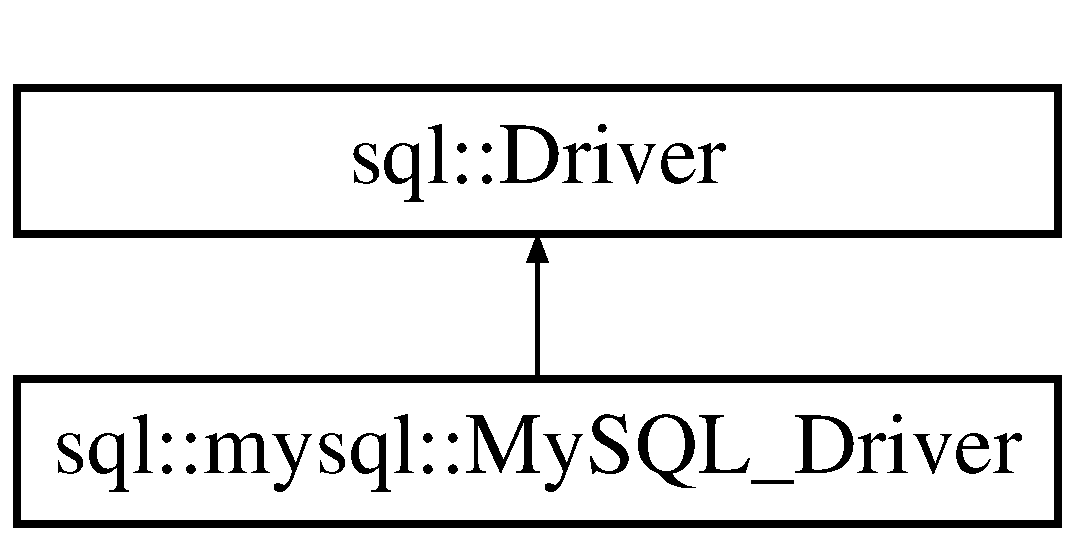
\includegraphics[height=2.000000cm]{classsql_1_1_driver}
\end{center}
\end{figure}
\subsection*{Public Member Functions}
\begin{DoxyCompactItemize}
\item 
\hypertarget{classsql_1_1_driver_a5dddccb95a32c265602b803d7a53d6a8}{}\label{classsql_1_1_driver_a5dddccb95a32c265602b803d7a53d6a8} 
virtual \hyperlink{classsql_1_1_connection}{Connection} $\ast$ {\bfseries connect} (const \hyperlink{classsql_1_1_s_q_l_string}{sql\+::\+S\+Q\+L\+String} \&host\+Name, const \hyperlink{classsql_1_1_s_q_l_string}{sql\+::\+S\+Q\+L\+String} \&user\+Name, const \hyperlink{classsql_1_1_s_q_l_string}{sql\+::\+S\+Q\+L\+String} \&password)=0
\item 
\hypertarget{classsql_1_1_driver_a20b70418563cf052a74a45d1ecb2187e}{}\label{classsql_1_1_driver_a20b70418563cf052a74a45d1ecb2187e} 
virtual \hyperlink{classsql_1_1_connection}{Connection} $\ast$ {\bfseries connect} (Connect\+Options\+Map \&options)=0
\item 
\hypertarget{classsql_1_1_driver_adbb7ba637734664d05a4abd8600347a3}{}\label{classsql_1_1_driver_adbb7ba637734664d05a4abd8600347a3} 
virtual int {\bfseries get\+Major\+Version} ()=0
\item 
\hypertarget{classsql_1_1_driver_a6f4d2599b74a49687281aff75d4e5ca3}{}\label{classsql_1_1_driver_a6f4d2599b74a49687281aff75d4e5ca3} 
virtual int {\bfseries get\+Minor\+Version} ()=0
\item 
\hypertarget{classsql_1_1_driver_ac4ed640d76190e68dfe79354b8431e24}{}\label{classsql_1_1_driver_ac4ed640d76190e68dfe79354b8431e24} 
virtual int {\bfseries get\+Patch\+Version} ()=0
\item 
\hypertarget{classsql_1_1_driver_a06d2dc9c3afdd160f7bbca73495d204a}{}\label{classsql_1_1_driver_a06d2dc9c3afdd160f7bbca73495d204a} 
virtual const \hyperlink{classsql_1_1_s_q_l_string}{sql\+::\+S\+Q\+L\+String} \& {\bfseries get\+Name} ()=0
\item 
\hypertarget{classsql_1_1_driver_acf4b00be0f101a438ed559cc642f5f54}{}\label{classsql_1_1_driver_acf4b00be0f101a438ed559cc642f5f54} 
virtual void {\bfseries thread\+Init} ()=0
\item 
\hypertarget{classsql_1_1_driver_a3bff3ef723874f9455e423472d08e630}{}\label{classsql_1_1_driver_a3bff3ef723874f9455e423472d08e630} 
virtual void {\bfseries thread\+End} ()=0
\end{DoxyCompactItemize}


The documentation for this class was generated from the following file\+:\begin{DoxyCompactItemize}
\item 
E\+:/projekt\+\_\+cpp\+\_\+magazyn/projekt/\+Magazyn/\+Magazyn/\+Magazyn/mysql/include/cppconn/driver.\+h\end{DoxyCompactItemize}

\hypertarget{structsql_1_1_invalid_argument_exception}{}\section{sql\+:\+:Invalid\+Argument\+Exception Struct Reference}
\label{structsql_1_1_invalid_argument_exception}\index{sql\+::\+Invalid\+Argument\+Exception@{sql\+::\+Invalid\+Argument\+Exception}}
Inheritance diagram for sql\+:\+:Invalid\+Argument\+Exception\+:\begin{figure}[H]
\begin{center}
\leavevmode
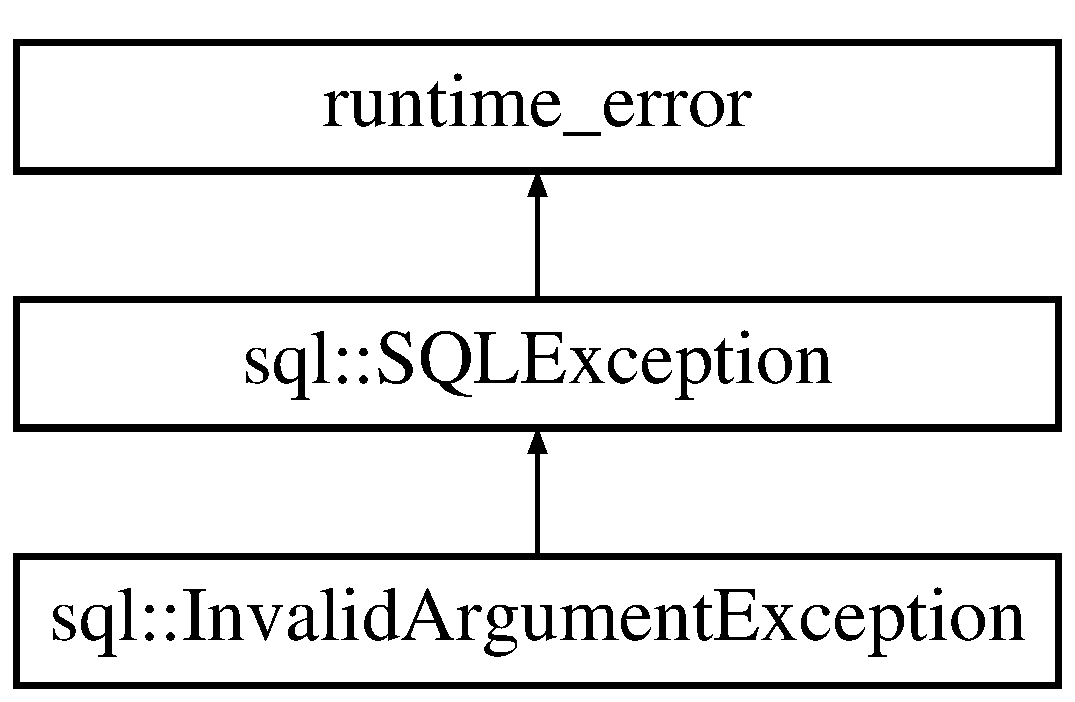
\includegraphics[height=3.000000cm]{structsql_1_1_invalid_argument_exception}
\end{center}
\end{figure}
\subsection*{Public Member Functions}
\begin{DoxyCompactItemize}
\item 
\hypertarget{structsql_1_1_invalid_argument_exception_a2598c1564255a696d5da59ffa76d8ad7}{}\label{structsql_1_1_invalid_argument_exception_a2598c1564255a696d5da59ffa76d8ad7} 
{\bfseries Invalid\+Argument\+Exception} (const \hyperlink{structsql_1_1_invalid_argument_exception}{Invalid\+Argument\+Exception} \&e)
\item 
\hypertarget{structsql_1_1_invalid_argument_exception_a3d98490d7f4ed27ea593983daa6d1aee}{}\label{structsql_1_1_invalid_argument_exception_a3d98490d7f4ed27ea593983daa6d1aee} 
{\bfseries Invalid\+Argument\+Exception} (const std\+::string \&reason)
\end{DoxyCompactItemize}
\subsection*{Additional Inherited Members}


The documentation for this struct was generated from the following file\+:\begin{DoxyCompactItemize}
\item 
E\+:/projekt\+\_\+cpp\+\_\+magazyn/projekt/\+Magazyn/\+Magazyn/\+Magazyn/mysql/include/cppconn/exception.\+h\end{DoxyCompactItemize}

\hypertarget{structsql_1_1_invalid_instance_exception}{}\section{sql\+:\+:Invalid\+Instance\+Exception Struct Reference}
\label{structsql_1_1_invalid_instance_exception}\index{sql\+::\+Invalid\+Instance\+Exception@{sql\+::\+Invalid\+Instance\+Exception}}
Inheritance diagram for sql\+:\+:Invalid\+Instance\+Exception\+:\begin{figure}[H]
\begin{center}
\leavevmode
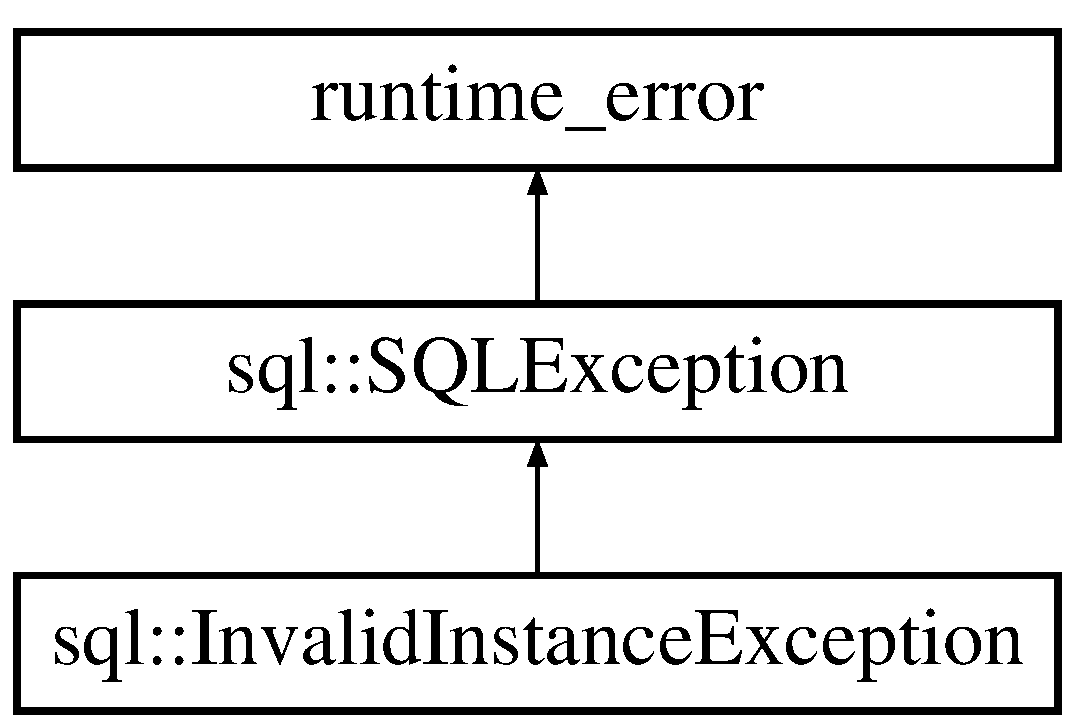
\includegraphics[height=3.000000cm]{structsql_1_1_invalid_instance_exception}
\end{center}
\end{figure}
\subsection*{Public Member Functions}
\begin{DoxyCompactItemize}
\item 
\hypertarget{structsql_1_1_invalid_instance_exception_ab05dca77f401255f0b4ec853251dfe1e}{}\label{structsql_1_1_invalid_instance_exception_ab05dca77f401255f0b4ec853251dfe1e} 
{\bfseries Invalid\+Instance\+Exception} (const \hyperlink{structsql_1_1_invalid_instance_exception}{Invalid\+Instance\+Exception} \&e)
\item 
\hypertarget{structsql_1_1_invalid_instance_exception_a37ad3895e8193a28d82fad885cfbdd89}{}\label{structsql_1_1_invalid_instance_exception_a37ad3895e8193a28d82fad885cfbdd89} 
{\bfseries Invalid\+Instance\+Exception} (const std\+::string \&reason)
\end{DoxyCompactItemize}
\subsection*{Additional Inherited Members}


The documentation for this struct was generated from the following file\+:\begin{DoxyCompactItemize}
\item 
E\+:/projekt\+\_\+cpp\+\_\+magazyn/projekt/\+Magazyn/\+Magazyn/\+Magazyn/mysql/include/cppconn/exception.\+h\end{DoxyCompactItemize}

\hypertarget{class_magazyn_1_1_login}{}\section{Magazyn\+:\+:Login Class Reference}
\label{class_magazyn_1_1_login}\index{Magazyn\+::\+Login@{Magazyn\+::\+Login}}


Summary for \hyperlink{class_magazyn_1_1_login}{Login}  




{\ttfamily \#include $<$Login.\+h$>$}

Inheritance diagram for Magazyn\+:\+:Login\+:\begin{figure}[H]
\begin{center}
\leavevmode
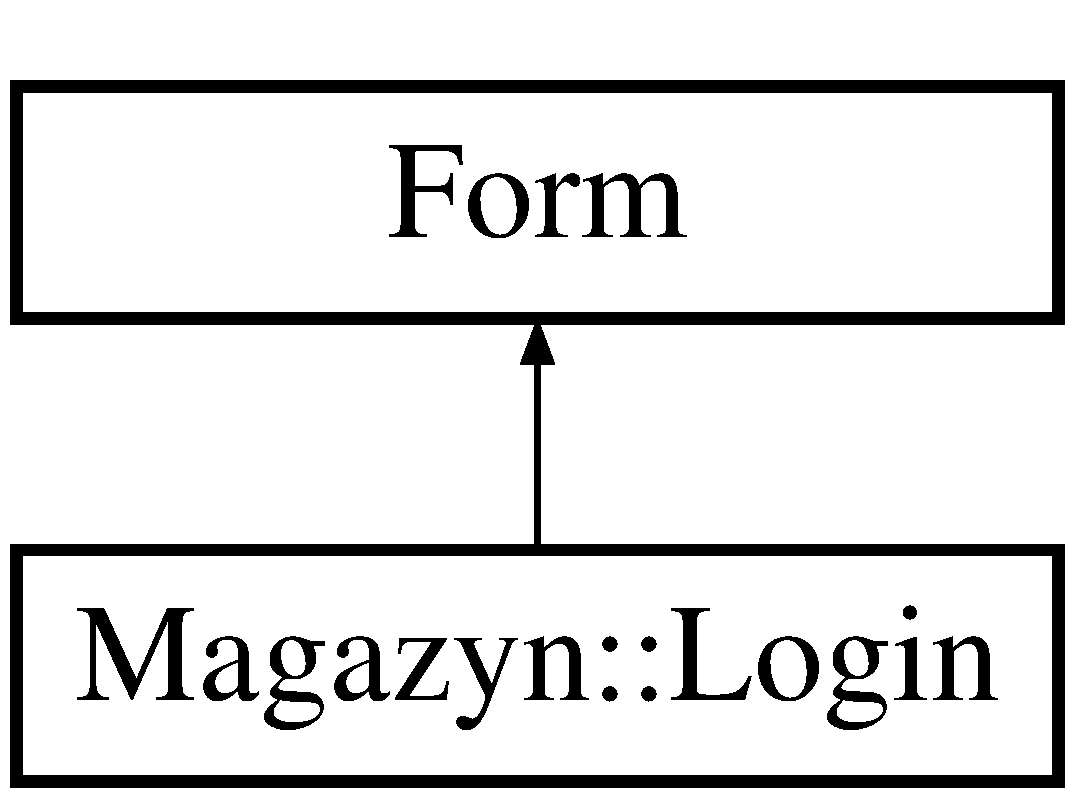
\includegraphics[height=2.000000cm]{class_magazyn_1_1_login}
\end{center}
\end{figure}
\subsection*{Protected Member Functions}
\begin{DoxyCompactItemize}
\item 
\hyperlink{class_magazyn_1_1_login_a421c32a7433145a0ed19b25b3ea87ddc}{$\sim$\+Login} ()
\begin{DoxyCompactList}\small\item\em Clean up any resources being used. \end{DoxyCompactList}\end{DoxyCompactItemize}
\subsection*{Private Member Functions}
\begin{DoxyCompactItemize}
\item 
void \hyperlink{class_magazyn_1_1_login_ac489095816b5d1b5fb33d523c3a4c59f}{Initialize\+Component} (void)
\begin{DoxyCompactList}\small\item\em Required method for Designer support -\/ do not modify the contents of this method with the code editor. \end{DoxyCompactList}\item 
\hypertarget{class_magazyn_1_1_login_a673cb544be89c23d940f3869461b9492}{}\label{class_magazyn_1_1_login_a673cb544be89c23d940f3869461b9492} 
System\+::\+Void {\bfseries btn\+Exit\+\_\+\+Click} (System\+::\+Object$^\wedge$ sender, System\+::\+Event\+Args$^\wedge$ e)
\item 
\hypertarget{class_magazyn_1_1_login_afc6385cc98691c04cef1aaf857c5c029}{}\label{class_magazyn_1_1_login_afc6385cc98691c04cef1aaf857c5c029} 
System\+::\+Void {\bfseries btn\+Login\+\_\+\+Click} (System\+::\+Object$^\wedge$ sender, System\+::\+Event\+Args$^\wedge$ e)
\end{DoxyCompactItemize}
\subsection*{Private Attributes}
\begin{DoxyCompactItemize}
\item 
\hypertarget{class_magazyn_1_1_login_adc89cc4a8bc3cacc4641ee99dd9addf8}{}\label{class_magazyn_1_1_login_adc89cc4a8bc3cacc4641ee99dd9addf8} 
System\+::\+Windows\+::\+Forms\+::\+Button {\bfseries btn\+Exit}
\item 
\hypertarget{class_magazyn_1_1_login_af7e6d68cdca548aaa1c34d0c5bdfa1b3}{}\label{class_magazyn_1_1_login_af7e6d68cdca548aaa1c34d0c5bdfa1b3} 
System\+::\+Windows\+::\+Forms\+::\+Button {\bfseries btn\+Login}
\item 
\hypertarget{class_magazyn_1_1_login_ab59428ff5c6bb8f811319492fb75c54a}{}\label{class_magazyn_1_1_login_ab59428ff5c6bb8f811319492fb75c54a} 
System\+::\+Windows\+::\+Forms\+::\+Text\+Box {\bfseries text\+Box\+Login}
\item 
\hypertarget{class_magazyn_1_1_login_a92053b5ae166b6d90f51d34cbc555574}{}\label{class_magazyn_1_1_login_a92053b5ae166b6d90f51d34cbc555574} 
System\+::\+Windows\+::\+Forms\+::\+Text\+Box {\bfseries text\+Box\+Password}
\item 
\hypertarget{class_magazyn_1_1_login_adb1872ac48717852b57a433661a7bf95}{}\label{class_magazyn_1_1_login_adb1872ac48717852b57a433661a7bf95} 
System\+::\+Windows\+::\+Forms\+::\+Label {\bfseries label\+Login}
\item 
\hypertarget{class_magazyn_1_1_login_a131f47ddc0a64ea34666db00455b9faa}{}\label{class_magazyn_1_1_login_a131f47ddc0a64ea34666db00455b9faa} 
System\+::\+Windows\+::\+Forms\+::\+Label {\bfseries label\+Password}
\item 
\hypertarget{class_magazyn_1_1_login_a7967ac4de79a64c6313c7e43efba7d40}{}\label{class_magazyn_1_1_login_a7967ac4de79a64c6313c7e43efba7d40} 
System\+::\+Windows\+::\+Forms\+::\+Label {\bfseries label\+Title}
\item 
System\+::\+Component\+Model\+::\+Container \hyperlink{class_magazyn_1_1_login_a2457e69b73940be27550fcfe3a8040c8}{components}
\begin{DoxyCompactList}\small\item\em Required designer variable. \end{DoxyCompactList}\end{DoxyCompactItemize}


\subsection{Detailed Description}
Summary for \hyperlink{class_magazyn_1_1_login}{Login} 



\subsection{Constructor \& Destructor Documentation}
\hypertarget{class_magazyn_1_1_login_a421c32a7433145a0ed19b25b3ea87ddc}{}\label{class_magazyn_1_1_login_a421c32a7433145a0ed19b25b3ea87ddc} 
\index{Magazyn\+::\+Login@{Magazyn\+::\+Login}!````~Login@{$\sim$\+Login}}
\index{````~Login@{$\sim$\+Login}!Magazyn\+::\+Login@{Magazyn\+::\+Login}}
\subsubsection{\texorpdfstring{$\sim$\+Login()}{~Login()}}
{\footnotesize\ttfamily Magazyn\+::\+Login\+::$\sim$\+Login (\begin{DoxyParamCaption}{ }\end{DoxyParamCaption})\hspace{0.3cm}{\ttfamily [inline]}, {\ttfamily [protected]}}



Clean up any resources being used. 



\subsection{Member Function Documentation}
\hypertarget{class_magazyn_1_1_login_ac489095816b5d1b5fb33d523c3a4c59f}{}\label{class_magazyn_1_1_login_ac489095816b5d1b5fb33d523c3a4c59f} 
\index{Magazyn\+::\+Login@{Magazyn\+::\+Login}!Initialize\+Component@{Initialize\+Component}}
\index{Initialize\+Component@{Initialize\+Component}!Magazyn\+::\+Login@{Magazyn\+::\+Login}}
\subsubsection{\texorpdfstring{Initialize\+Component()}{InitializeComponent()}}
{\footnotesize\ttfamily void Magazyn\+::\+Login\+::\+Initialize\+Component (\begin{DoxyParamCaption}\item[{void}]{ }\end{DoxyParamCaption})\hspace{0.3cm}{\ttfamily [inline]}, {\ttfamily [private]}}



Required method for Designer support -\/ do not modify the contents of this method with the code editor. 



\subsection{Member Data Documentation}
\hypertarget{class_magazyn_1_1_login_a2457e69b73940be27550fcfe3a8040c8}{}\label{class_magazyn_1_1_login_a2457e69b73940be27550fcfe3a8040c8} 
\index{Magazyn\+::\+Login@{Magazyn\+::\+Login}!components@{components}}
\index{components@{components}!Magazyn\+::\+Login@{Magazyn\+::\+Login}}
\subsubsection{\texorpdfstring{components}{components}}
{\footnotesize\ttfamily System\+::\+Component\+Model\+::\+Container Magazyn\+::\+Login\+::components\hspace{0.3cm}{\ttfamily [private]}}



Required designer variable. 



The documentation for this class was generated from the following file\+:\begin{DoxyCompactItemize}
\item 
E\+:/projekt\+\_\+cpp\+\_\+magazyn/projekt/\+Magazyn/\+Magazyn/\+Magazyn/Login.\+h\end{DoxyCompactItemize}

\hypertarget{class_magazyn_1_1_magazin}{}\section{Magazyn\+:\+:Magazin Class Reference}
\label{class_magazyn_1_1_magazin}\index{Magazyn\+::\+Magazin@{Magazyn\+::\+Magazin}}


Summary for \hyperlink{class_magazyn_1_1_magazin}{Magazin}  




{\ttfamily \#include $<$Magazin.\+h$>$}

Inheritance diagram for Magazyn\+:\+:Magazin\+:\begin{figure}[H]
\begin{center}
\leavevmode
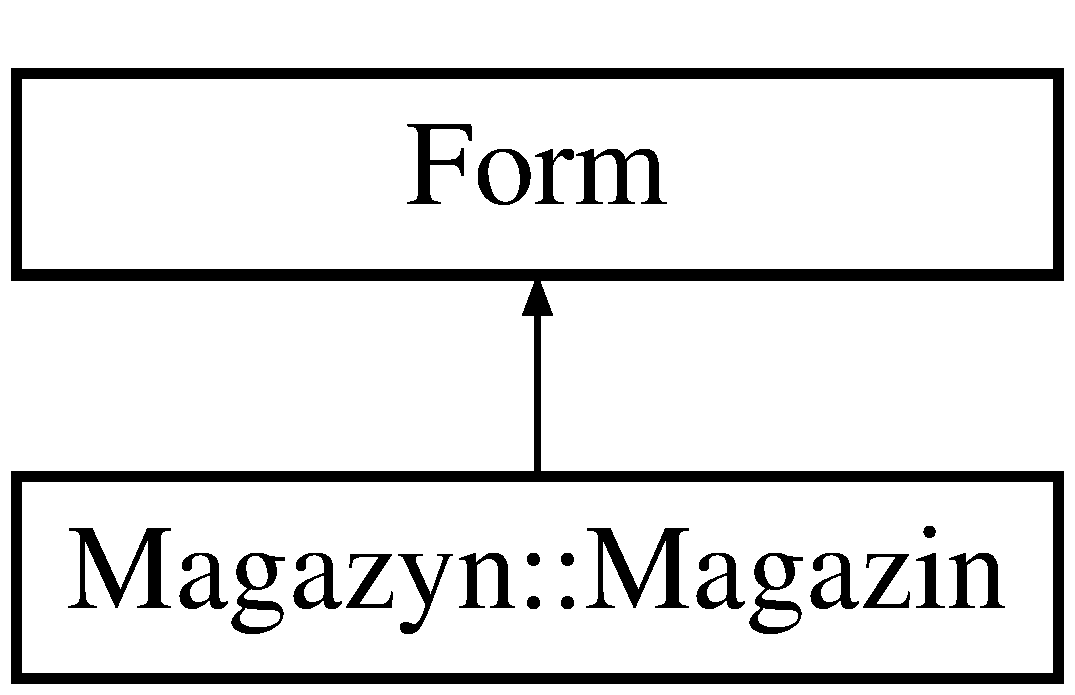
\includegraphics[height=2.000000cm]{class_magazyn_1_1_magazin}
\end{center}
\end{figure}
\subsection*{Public Member Functions}
\begin{DoxyCompactItemize}
\item 
\hypertarget{class_magazyn_1_1_magazin_aa115a58816655e83d9a067d8c840a3e9}{}\label{class_magazyn_1_1_magazin_aa115a58816655e83d9a067d8c840a3e9} 
{\bfseries Magazin} (int user\+Id\+From\+Login)
\end{DoxyCompactItemize}
\subsection*{Protected Member Functions}
\begin{DoxyCompactItemize}
\item 
\hyperlink{class_magazyn_1_1_magazin_a3d5a3139a7bce989a8cff474eaa311d6}{$\sim$\+Magazin} ()
\begin{DoxyCompactList}\small\item\em Clean up any resources being used. \end{DoxyCompactList}\end{DoxyCompactItemize}
\subsection*{Private Member Functions}
\begin{DoxyCompactItemize}
\item 
void \hyperlink{class_magazyn_1_1_magazin_a99d47c14fc619cce7d7b5a9ca5c2ebe3}{Initialize\+Component} (void)
\begin{DoxyCompactList}\small\item\em Required method for Designer support -\/ do not modify the contents of this method with the code editor. \end{DoxyCompactList}\item 
\hypertarget{class_magazyn_1_1_magazin_a2ad7fe1375419739a695465f414638d8}{}\label{class_magazyn_1_1_magazin_a2ad7fe1375419739a695465f414638d8} 
System\+::\+Void {\bfseries Magazin\+\_\+\+Load} (System\+::\+Object$^\wedge$ sender, System\+::\+Event\+Args$^\wedge$ e)
\item 
\hypertarget{class_magazyn_1_1_magazin_a37a58617166481649855eb4867db0b86}{}\label{class_magazyn_1_1_magazin_a37a58617166481649855eb4867db0b86} 
Void {\bfseries bind\+All\+Tables} ()
\item 
\hypertarget{class_magazyn_1_1_magazin_ac836f9c7837b13f5adbc01a73f5f161c}{}\label{class_magazyn_1_1_magazin_ac836f9c7837b13f5adbc01a73f5f161c} 
Void {\bfseries bind\+Table} (String$^\wedge$ query, System\+::\+Windows\+::\+Forms\+::\+Data\+Grid\+View$^\wedge$ table)
\item 
\hypertarget{class_magazyn_1_1_magazin_a0d0ba5c93832afc9cd1ecb6b0e14bc06}{}\label{class_magazyn_1_1_magazin_a0d0ba5c93832afc9cd1ecb6b0e14bc06} 
System\+::\+Void {\bfseries btn\+Search\+Employers\+\_\+\+Click} (System\+::\+Object$^\wedge$ sender, System\+::\+Event\+Args$^\wedge$ e)
\item 
\hypertarget{class_magazyn_1_1_magazin_ae1902458a4bf62efc0b39051f76605fa}{}\label{class_magazyn_1_1_magazin_ae1902458a4bf62efc0b39051f76605fa} 
System\+::\+Void {\bfseries btn\+Show\+Employers\+\_\+\+Click} (System\+::\+Object$^\wedge$ sender, System\+::\+Event\+Args$^\wedge$ e)
\item 
\hypertarget{class_magazyn_1_1_magazin_a440db111753f8946a6f1a1cbb289a8d5}{}\label{class_magazyn_1_1_magazin_a440db111753f8946a6f1a1cbb289a8d5} 
System\+::\+Void {\bfseries table\+Employers\+\_\+\+Cell\+Click} (System\+::\+Object$^\wedge$ sender, System\+::\+Windows\+::\+Forms\+::\+Data\+Grid\+View\+Cell\+Event\+Args$^\wedge$ e)
\item 
\hypertarget{class_magazyn_1_1_magazin_a4d068e231b209d741fb79d5a8b0d32a0}{}\label{class_magazyn_1_1_magazin_a4d068e231b209d741fb79d5a8b0d32a0} 
System\+::\+Void {\bfseries btn\+Save\+Employer\+\_\+\+Click} (System\+::\+Object$^\wedge$ sender, System\+::\+Event\+Args$^\wedge$ e)
\item 
\hypertarget{class_magazyn_1_1_magazin_a9971c31701c92ea5fcec653dabd0c3d6}{}\label{class_magazyn_1_1_magazin_a9971c31701c92ea5fcec653dabd0c3d6} 
System\+::\+Void {\bfseries button\+Clear\+Form\+\_\+\+Click} (System\+::\+Object$^\wedge$ sender, System\+::\+Event\+Args$^\wedge$ e)
\item 
\hypertarget{class_magazyn_1_1_magazin_ac906afd7e120d985b4af877361104411}{}\label{class_magazyn_1_1_magazin_ac906afd7e120d985b4af877361104411} 
Void {\bfseries clear\+Form} ()
\item 
\hypertarget{class_magazyn_1_1_magazin_a0b48230c0e70b52f31c94dcef82a5cc0}{}\label{class_magazyn_1_1_magazin_a0b48230c0e70b52f31c94dcef82a5cc0} 
System\+::\+Void {\bfseries button\+Employer\+Delete\+\_\+\+Click} (System\+::\+Object$^\wedge$ sender, System\+::\+Event\+Args$^\wedge$ e)
\item 
\hypertarget{class_magazyn_1_1_magazin_a3bf8949bf6505ac5f26b4a96c94190ab}{}\label{class_magazyn_1_1_magazin_a3bf8949bf6505ac5f26b4a96c94190ab} 
System\+::\+Void {\bfseries Magazin\+\_\+\+Form\+Closing} (System\+::\+Object$^\wedge$ sender, System\+::\+Windows\+::\+Forms\+::\+Form\+Closing\+Event\+Args$^\wedge$ e)
\item 
\hypertarget{class_magazyn_1_1_magazin_ace66b19ac457b029ecb6bf3eb5b4732e}{}\label{class_magazyn_1_1_magazin_ace66b19ac457b029ecb6bf3eb5b4732e} 
Void {\bfseries account\+Settings} ()
\item 
\hypertarget{class_magazyn_1_1_magazin_a2b139e400b26519295b79da050883305}{}\label{class_magazyn_1_1_magazin_a2b139e400b26519295b79da050883305} 
System\+::\+Void {\bfseries button1\+\_\+\+Click} (System\+::\+Object$^\wedge$ sender, System\+::\+Event\+Args$^\wedge$ e)
\item 
\hypertarget{class_magazyn_1_1_magazin_a57fb0148d5d70a0e9dc970d6016c7e73}{}\label{class_magazyn_1_1_magazin_a57fb0148d5d70a0e9dc970d6016c7e73} 
System\+::\+Void {\bfseries button\+Show\+Clients\+\_\+\+Click} (System\+::\+Object$^\wedge$ sender, System\+::\+Event\+Args$^\wedge$ e)
\item 
\hypertarget{class_magazyn_1_1_magazin_add4f3f7e4935b77ffd9c1107d13c04ee}{}\label{class_magazyn_1_1_magazin_add4f3f7e4935b77ffd9c1107d13c04ee} 
System\+::\+Void {\bfseries button\+Search\+Clients\+\_\+\+Click} (System\+::\+Object$^\wedge$ sender, System\+::\+Event\+Args$^\wedge$ e)
\item 
\hypertarget{class_magazyn_1_1_magazin_aefe821059189a7fc8af1e03dd595b503}{}\label{class_magazyn_1_1_magazin_aefe821059189a7fc8af1e03dd595b503} 
System\+::\+Void {\bfseries data\+Grid\+View\+Clients\+\_\+\+Cell\+Click} (System\+::\+Object$^\wedge$ sender, System\+::\+Windows\+::\+Forms\+::\+Data\+Grid\+View\+Cell\+Event\+Args$^\wedge$ e)
\item 
\hypertarget{class_magazyn_1_1_magazin_a8271e54ebbfc0fc18c3e903ce0b47aaa}{}\label{class_magazyn_1_1_magazin_a8271e54ebbfc0fc18c3e903ce0b47aaa} 
System\+::\+Void {\bfseries button\+Clear\+Form\+Client\+\_\+\+Click} (System\+::\+Object$^\wedge$ sender, System\+::\+Event\+Args$^\wedge$ e)
\item 
\hypertarget{class_magazyn_1_1_magazin_ae27a37e927bc66580166fca7cfd00b1c}{}\label{class_magazyn_1_1_magazin_ae27a37e927bc66580166fca7cfd00b1c} 
Void {\bfseries clear\+Form\+Clients} ()
\item 
\hypertarget{class_magazyn_1_1_magazin_a86c5d71826074381ee41a62fce8e4319}{}\label{class_magazyn_1_1_magazin_a86c5d71826074381ee41a62fce8e4319} 
System\+::\+Void {\bfseries button\+Save\+Client\+\_\+\+Click} (System\+::\+Object$^\wedge$ sender, System\+::\+Event\+Args$^\wedge$ e)
\item 
\hypertarget{class_magazyn_1_1_magazin_a98742314d98306613e3ef1ca45216373}{}\label{class_magazyn_1_1_magazin_a98742314d98306613e3ef1ca45216373} 
System\+::\+Void {\bfseries button\+Delete\+Client\+\_\+\+Click} (System\+::\+Object$^\wedge$ sender, System\+::\+Event\+Args$^\wedge$ e)
\item 
\hypertarget{class_magazyn_1_1_magazin_a3ae2fcfc8a09e15089f9b7ed4f7e5e99}{}\label{class_magazyn_1_1_magazin_a3ae2fcfc8a09e15089f9b7ed4f7e5e99} 
System\+::\+Void {\bfseries button\+Show\+Providers\+\_\+\+Click} (System\+::\+Object$^\wedge$ sender, System\+::\+Event\+Args$^\wedge$ e)
\item 
\hypertarget{class_magazyn_1_1_magazin_a9c121ceaa80423f04e40ff553350f845}{}\label{class_magazyn_1_1_magazin_a9c121ceaa80423f04e40ff553350f845} 
System\+::\+Void {\bfseries button\+Search\+Providers\+\_\+\+Click} (System\+::\+Object$^\wedge$ sender, System\+::\+Event\+Args$^\wedge$ e)
\item 
\hypertarget{class_magazyn_1_1_magazin_adf2683e579e6cd3cfe68f47530928e87}{}\label{class_magazyn_1_1_magazin_adf2683e579e6cd3cfe68f47530928e87} 
System\+::\+Void {\bfseries data\+Grid\+View\+Providers\+\_\+\+Cell\+Click} (System\+::\+Object$^\wedge$ sender, System\+::\+Windows\+::\+Forms\+::\+Data\+Grid\+View\+Cell\+Event\+Args$^\wedge$ e)
\item 
\hypertarget{class_magazyn_1_1_magazin_aa289ab59d38376ffbbf5f9286aedc8a2}{}\label{class_magazyn_1_1_magazin_aa289ab59d38376ffbbf5f9286aedc8a2} 
System\+::\+Void {\bfseries button\+Clear\+Provider\+Form\+\_\+\+Click} (System\+::\+Object$^\wedge$ sender, System\+::\+Event\+Args$^\wedge$ e)
\item 
\hypertarget{class_magazyn_1_1_magazin_af1f8f28a803fa1dfc5820c89501a93ae}{}\label{class_magazyn_1_1_magazin_af1f8f28a803fa1dfc5820c89501a93ae} 
Void {\bfseries clear\+Form\+Providers} ()
\item 
\hypertarget{class_magazyn_1_1_magazin_a1b33449d6353faf2ffca5ebb45a26d77}{}\label{class_magazyn_1_1_magazin_a1b33449d6353faf2ffca5ebb45a26d77} 
System\+::\+Void {\bfseries button\+Provider\+Save\+\_\+\+Click} (System\+::\+Object$^\wedge$ sender, System\+::\+Event\+Args$^\wedge$ e)
\item 
\hypertarget{class_magazyn_1_1_magazin_a121869cc605287e6d13f8767e1951512}{}\label{class_magazyn_1_1_magazin_a121869cc605287e6d13f8767e1951512} 
System\+::\+Void {\bfseries button\+Provider\+Delete\+\_\+\+Click} (System\+::\+Object$^\wedge$ sender, System\+::\+Event\+Args$^\wedge$ e)
\item 
\hypertarget{class_magazyn_1_1_magazin_af8d814868f0b91db7ec19b7c65a9458d}{}\label{class_magazyn_1_1_magazin_af8d814868f0b91db7ec19b7c65a9458d} 
System\+::\+Void {\bfseries button\+Items\+Show\+\_\+\+Click} (System\+::\+Object$^\wedge$ sender, System\+::\+Event\+Args$^\wedge$ e)
\item 
\hypertarget{class_magazyn_1_1_magazin_aeedf3f5f79926aaf9a5287e588806419}{}\label{class_magazyn_1_1_magazin_aeedf3f5f79926aaf9a5287e588806419} 
System\+::\+Void {\bfseries button\+Items\+Search\+\_\+\+Click} (System\+::\+Object$^\wedge$ sender, System\+::\+Event\+Args$^\wedge$ e)
\item 
\hypertarget{class_magazyn_1_1_magazin_a9976f63514d0e56c82c9a36a386df804}{}\label{class_magazyn_1_1_magazin_a9976f63514d0e56c82c9a36a386df804} 
System\+::\+Void {\bfseries data\+Grid\+View\+Items\+\_\+\+Cell\+Click} (System\+::\+Object$^\wedge$ sender, System\+::\+Windows\+::\+Forms\+::\+Data\+Grid\+View\+Cell\+Event\+Args$^\wedge$ e)
\item 
\hypertarget{class_magazyn_1_1_magazin_a4952a20bc553e0b94949f779bd4d6d5c}{}\label{class_magazyn_1_1_magazin_a4952a20bc553e0b94949f779bd4d6d5c} 
System\+::\+Void {\bfseries combo\+Box\+Item\+Param\+\_\+\+Selected\+Index\+Changed} (System\+::\+Object$^\wedge$ sender, System\+::\+Event\+Args$^\wedge$ e)
\item 
\hypertarget{class_magazyn_1_1_magazin_a43c3506c415fae23e2026ee1668d6284}{}\label{class_magazyn_1_1_magazin_a43c3506c415fae23e2026ee1668d6284} 
System\+::\+Void {\bfseries button\+Item\+Clear\+Form\+\_\+\+Click} (System\+::\+Object$^\wedge$ sender, System\+::\+Event\+Args$^\wedge$ e)
\item 
\hypertarget{class_magazyn_1_1_magazin_ae8eaea84ec62af014904e6ea941d418f}{}\label{class_magazyn_1_1_magazin_ae8eaea84ec62af014904e6ea941d418f} 
Void {\bfseries clear\+Item\+Form} ()
\item 
\hypertarget{class_magazyn_1_1_magazin_a3cc415a7ff1f948ad064058868303f0f}{}\label{class_magazyn_1_1_magazin_a3cc415a7ff1f948ad064058868303f0f} 
System\+::\+Void {\bfseries button\+Item\+Save\+\_\+\+Click} (System\+::\+Object$^\wedge$ sender, System\+::\+Event\+Args$^\wedge$ e)
\item 
\hypertarget{class_magazyn_1_1_magazin_a7cb15f12b46223355e42333f67c5b6ff}{}\label{class_magazyn_1_1_magazin_a7cb15f12b46223355e42333f67c5b6ff} 
System\+::\+Void {\bfseries button\+Item\+Param\+Add\+\_\+\+Click} (System\+::\+Object$^\wedge$ sender, System\+::\+Event\+Args$^\wedge$ e)
\item 
\hypertarget{class_magazyn_1_1_magazin_a112455c9a1b5f08b85544abf2cbfb906}{}\label{class_magazyn_1_1_magazin_a112455c9a1b5f08b85544abf2cbfb906} 
System\+::\+Void {\bfseries button\+Item\+Param\+Delete\+\_\+\+Click} (System\+::\+Object$^\wedge$ sender, System\+::\+Event\+Args$^\wedge$ e)
\item 
\hypertarget{class_magazyn_1_1_magazin_a633c56775a43b9b7e8b5be63f7814e08}{}\label{class_magazyn_1_1_magazin_a633c56775a43b9b7e8b5be63f7814e08} 
System\+::\+Void {\bfseries button\+Item\+Producer\+Add\+\_\+\+Click} (System\+::\+Object$^\wedge$ sender, System\+::\+Event\+Args$^\wedge$ e)
\item 
\hypertarget{class_magazyn_1_1_magazin_a811b8f04e245301b0da541c8d6bd73a9}{}\label{class_magazyn_1_1_magazin_a811b8f04e245301b0da541c8d6bd73a9} 
System\+::\+Void {\bfseries button\+Item\+Producer\+Delete\+\_\+\+Click} (System\+::\+Object$^\wedge$ sender, System\+::\+Event\+Args$^\wedge$ e)
\item 
\hypertarget{class_magazyn_1_1_magazin_ab61f7ce6732b6fd67e6b0871087ce5df}{}\label{class_magazyn_1_1_magazin_ab61f7ce6732b6fd67e6b0871087ce5df} 
System\+::\+Void {\bfseries button\+Item\+Delete\+\_\+\+Click} (System\+::\+Object$^\wedge$ sender, System\+::\+Event\+Args$^\wedge$ e)
\item 
\hypertarget{class_magazyn_1_1_magazin_a142c4fbd25886c879895c7c5df898643}{}\label{class_magazyn_1_1_magazin_a142c4fbd25886c879895c7c5df898643} 
System\+::\+Void {\bfseries button\+Item\+Help\+\_\+\+Click} (System\+::\+Object$^\wedge$ sender, System\+::\+Event\+Args$^\wedge$ e)
\item 
\hypertarget{class_magazyn_1_1_magazin_a38bf656bd772b4f6fdecf4ec12c4ec2b}{}\label{class_magazyn_1_1_magazin_a38bf656bd772b4f6fdecf4ec12c4ec2b} 
System\+::\+Void {\bfseries button\+Item\+Param\+Help\+\_\+\+Click} (System\+::\+Object$^\wedge$ sender, System\+::\+Event\+Args$^\wedge$ e)
\item 
\hypertarget{class_magazyn_1_1_magazin_ad14b33f28c78af93c07d61507ec82d13}{}\label{class_magazyn_1_1_magazin_ad14b33f28c78af93c07d61507ec82d13} 
System\+::\+Void {\bfseries button\+Item\+Producer\+Help\+\_\+\+Click} (System\+::\+Object$^\wedge$ sender, System\+::\+Event\+Args$^\wedge$ e)
\item 
\hypertarget{class_magazyn_1_1_magazin_ae23692db5f25cc766e5bd6214354cfb2}{}\label{class_magazyn_1_1_magazin_ae23692db5f25cc766e5bd6214354cfb2} 
System\+::\+Void {\bfseries button\+Sells\+Show\+\_\+\+Click} (System\+::\+Object$^\wedge$ sender, System\+::\+Event\+Args$^\wedge$ e)
\item 
\hypertarget{class_magazyn_1_1_magazin_ab8d1673031a48aefbd7dfcfcb951393d}{}\label{class_magazyn_1_1_magazin_ab8d1673031a48aefbd7dfcfcb951393d} 
System\+::\+Void {\bfseries button\+Sales\+Save\+\_\+\+Click} (System\+::\+Object$^\wedge$ sender, System\+::\+Event\+Args$^\wedge$ e)
\item 
\hypertarget{class_magazyn_1_1_magazin_a29c710017ebfa3a262931fba0b75f316}{}\label{class_magazyn_1_1_magazin_a29c710017ebfa3a262931fba0b75f316} 
System\+::\+Void {\bfseries data\+Grid\+View\+Sales\+\_\+\+Cell\+Click} (System\+::\+Object$^\wedge$ sender, System\+::\+Windows\+::\+Forms\+::\+Data\+Grid\+View\+Cell\+Event\+Args$^\wedge$ e)
\item 
\hypertarget{class_magazyn_1_1_magazin_a276657fae69adc303e1c88b4441b3e47}{}\label{class_magazyn_1_1_magazin_a276657fae69adc303e1c88b4441b3e47} 
System\+::\+Void {\bfseries combo\+Box\+Sell\+Client\+\_\+\+Selected\+Index\+Changed} (System\+::\+Object$^\wedge$ sender, System\+::\+Event\+Args$^\wedge$ e)
\item 
\hypertarget{class_magazyn_1_1_magazin_aaa3f43ca8cd10efe0358e70258822e37}{}\label{class_magazyn_1_1_magazin_aaa3f43ca8cd10efe0358e70258822e37} 
System\+::\+Void {\bfseries button\+Sales\+Add\+Item\+\_\+\+Click} (System\+::\+Object$^\wedge$ sender, System\+::\+Event\+Args$^\wedge$ e)
\item 
\hypertarget{class_magazyn_1_1_magazin_a27eca229d3b3cff68414eb63c62964d2}{}\label{class_magazyn_1_1_magazin_a27eca229d3b3cff68414eb63c62964d2} 
System\+::\+Void {\bfseries combo\+Box\+Sell\+Item\+\_\+\+Selected\+Index\+Changed} (System\+::\+Object$^\wedge$ sender, System\+::\+Event\+Args$^\wedge$ e)
\item 
\hypertarget{class_magazyn_1_1_magazin_a19664754d090eaf27da1b466bcf0fb43}{}\label{class_magazyn_1_1_magazin_a19664754d090eaf27da1b466bcf0fb43} 
System\+::\+Void {\bfseries button\+Sales\+Delete\+Item\+\_\+\+Click} (System\+::\+Object$^\wedge$ sender, System\+::\+Event\+Args$^\wedge$ e)
\item 
\hypertarget{class_magazyn_1_1_magazin_a0f1b3f4da16de2da70c5b5cca1ad4eb9}{}\label{class_magazyn_1_1_magazin_a0f1b3f4da16de2da70c5b5cca1ad4eb9} 
System\+::\+Void {\bfseries data\+Grid\+View\+Sales\+Items\+\_\+\+Cell\+Click} (System\+::\+Object$^\wedge$ sender, System\+::\+Windows\+::\+Forms\+::\+Data\+Grid\+View\+Cell\+Event\+Args$^\wedge$ e)
\item 
\hypertarget{class_magazyn_1_1_magazin_a0160af3b98739778c1e2e1312d31d994}{}\label{class_magazyn_1_1_magazin_a0160af3b98739778c1e2e1312d31d994} 
System\+::\+Void {\bfseries button\+Sales\+Close\+\_\+\+Click} (System\+::\+Object$^\wedge$ sender, System\+::\+Event\+Args$^\wedge$ e)
\item 
\hypertarget{class_magazyn_1_1_magazin_a96f1e7d9daf88de45ec2a76e2df19b10}{}\label{class_magazyn_1_1_magazin_a96f1e7d9daf88de45ec2a76e2df19b10} 
System\+::\+Void {\bfseries button\+Sales\+Delete\+\_\+\+Click} (System\+::\+Object$^\wedge$ sender, System\+::\+Event\+Args$^\wedge$ e)
\item 
\hypertarget{class_magazyn_1_1_magazin_a6d6d6e6a61a4880994aad40e206e0364}{}\label{class_magazyn_1_1_magazin_a6d6d6e6a61a4880994aad40e206e0364} 
System\+::\+Void {\bfseries button\+Sales\+Clear\+Form\+\_\+\+Click} (System\+::\+Object$^\wedge$ sender, System\+::\+Event\+Args$^\wedge$ e)
\item 
\hypertarget{class_magazyn_1_1_magazin_ade058b3ee5433620fad999b81f71af39}{}\label{class_magazyn_1_1_magazin_ade058b3ee5433620fad999b81f71af39} 
Void {\bfseries clear\+Form\+Sales} ()
\item 
\hypertarget{class_magazyn_1_1_magazin_aef618ab780d3b4ad6b44bf93140cf878}{}\label{class_magazyn_1_1_magazin_aef618ab780d3b4ad6b44bf93140cf878} 
System\+::\+Void {\bfseries data\+Grid\+View\+Sales\+Clients\+\_\+\+Cell\+Click} (System\+::\+Object$^\wedge$ sender, System\+::\+Windows\+::\+Forms\+::\+Data\+Grid\+View\+Cell\+Event\+Args$^\wedge$ e)
\item 
\hypertarget{class_magazyn_1_1_magazin_a09b94963cdf1a63ff1f922b798a205f9}{}\label{class_magazyn_1_1_magazin_a09b94963cdf1a63ff1f922b798a205f9} 
System\+::\+Void {\bfseries data\+Grid\+View\+Sales\+Employers\+\_\+\+Cell\+Click} (System\+::\+Object$^\wedge$ sender, System\+::\+Windows\+::\+Forms\+::\+Data\+Grid\+View\+Cell\+Event\+Args$^\wedge$ e)
\item 
\hypertarget{class_magazyn_1_1_magazin_a61b6abbde1a270bb6ea6c5acd33cfbb3}{}\label{class_magazyn_1_1_magazin_a61b6abbde1a270bb6ea6c5acd33cfbb3} 
System\+::\+Void {\bfseries button\+Sales\+Help\+\_\+\+Click} (System\+::\+Object$^\wedge$ sender, System\+::\+Event\+Args$^\wedge$ e)
\item 
\hypertarget{class_magazyn_1_1_magazin_a470525112231ed90bb4b3490afef0191}{}\label{class_magazyn_1_1_magazin_a470525112231ed90bb4b3490afef0191} 
System\+::\+Void {\bfseries button\+Delivery\+Show\+\_\+\+Click} (System\+::\+Object$^\wedge$ sender, System\+::\+Event\+Args$^\wedge$ e)
\item 
\hypertarget{class_magazyn_1_1_magazin_a36d9c12155e637b02e57d4e03c64f850}{}\label{class_magazyn_1_1_magazin_a36d9c12155e637b02e57d4e03c64f850} 
System\+::\+Void {\bfseries button\+Delivery\+Save\+\_\+\+Click} (System\+::\+Object$^\wedge$ sender, System\+::\+Event\+Args$^\wedge$ e)
\item 
\hypertarget{class_magazyn_1_1_magazin_a63f39976669473311f0d90f0ebe77425}{}\label{class_magazyn_1_1_magazin_a63f39976669473311f0d90f0ebe77425} 
System\+::\+Void {\bfseries data\+Grid\+View\+Delivery\+\_\+\+Cell\+Click} (System\+::\+Object$^\wedge$ sender, System\+::\+Windows\+::\+Forms\+::\+Data\+Grid\+View\+Cell\+Event\+Args$^\wedge$ e)
\item 
\hypertarget{class_magazyn_1_1_magazin_a65f10a20ee2ec7e9bd61f135a9a6a6db}{}\label{class_magazyn_1_1_magazin_a65f10a20ee2ec7e9bd61f135a9a6a6db} 
System\+::\+Void {\bfseries combo\+Box\+Delivery\+Provider\+\_\+\+Selected\+Index\+Changed} (System\+::\+Object$^\wedge$ sender, System\+::\+Event\+Args$^\wedge$ e)
\item 
\hypertarget{class_magazyn_1_1_magazin_afc5fd76c2e80b61860792e888ca95a82}{}\label{class_magazyn_1_1_magazin_afc5fd76c2e80b61860792e888ca95a82} 
System\+::\+Void {\bfseries button\+Delivery\+Add\+Item\+\_\+\+Click} (System\+::\+Object$^\wedge$ sender, System\+::\+Event\+Args$^\wedge$ e)
\item 
\hypertarget{class_magazyn_1_1_magazin_aa37b356b4140df20b260b34162d7a6db}{}\label{class_magazyn_1_1_magazin_aa37b356b4140df20b260b34162d7a6db} 
System\+::\+Void {\bfseries combo\+Box\+Delivery\+Item\+\_\+\+Selected\+Index\+Changed} (System\+::\+Object$^\wedge$ sender, System\+::\+Event\+Args$^\wedge$ e)
\item 
\hypertarget{class_magazyn_1_1_magazin_a307440a9f7c2637db65bef29896cb339}{}\label{class_magazyn_1_1_magazin_a307440a9f7c2637db65bef29896cb339} 
System\+::\+Void {\bfseries button\+Delivery\+Delete\+Item\+\_\+\+Click} (System\+::\+Object$^\wedge$ sender, System\+::\+Event\+Args$^\wedge$ e)
\item 
\hypertarget{class_magazyn_1_1_magazin_a9329270816afd8fbdece19e8165e760d}{}\label{class_magazyn_1_1_magazin_a9329270816afd8fbdece19e8165e760d} 
System\+::\+Void {\bfseries data\+Grid\+View\+Delivery\+Items\+\_\+\+Cell\+Click} (System\+::\+Object$^\wedge$ sender, System\+::\+Windows\+::\+Forms\+::\+Data\+Grid\+View\+Cell\+Event\+Args$^\wedge$ e)
\item 
\hypertarget{class_magazyn_1_1_magazin_a67afa788e7c215ccc92963fe01709724}{}\label{class_magazyn_1_1_magazin_a67afa788e7c215ccc92963fe01709724} 
System\+::\+Void {\bfseries button\+Delivery\+Close\+\_\+\+Click} (System\+::\+Object$^\wedge$ sender, System\+::\+Event\+Args$^\wedge$ e)
\item 
\hypertarget{class_magazyn_1_1_magazin_a2779075855f3a65430f39561f362482d}{}\label{class_magazyn_1_1_magazin_a2779075855f3a65430f39561f362482d} 
System\+::\+Void {\bfseries button\+Delivery\+Delete\+\_\+\+Click} (System\+::\+Object$^\wedge$ sender, System\+::\+Event\+Args$^\wedge$ e)
\item 
\hypertarget{class_magazyn_1_1_magazin_aec5d557e622df716c8acf7a169ac18b9}{}\label{class_magazyn_1_1_magazin_aec5d557e622df716c8acf7a169ac18b9} 
System\+::\+Void {\bfseries button\+Delivery\+Clear\+Form\+\_\+\+Click} (System\+::\+Object$^\wedge$ sender, System\+::\+Event\+Args$^\wedge$ e)
\item 
\hypertarget{class_magazyn_1_1_magazin_a957014be87dcc6cbdbcda375872ef5be}{}\label{class_magazyn_1_1_magazin_a957014be87dcc6cbdbcda375872ef5be} 
Void {\bfseries clear\+Form\+Delivery} ()
\item 
\hypertarget{class_magazyn_1_1_magazin_a061791cc8134d6e273bde508633c0169}{}\label{class_magazyn_1_1_magazin_a061791cc8134d6e273bde508633c0169} 
System\+::\+Void {\bfseries data\+Grid\+View\+Delivery\+Providers\+\_\+\+Cell\+Click} (System\+::\+Object$^\wedge$ sender, System\+::\+Windows\+::\+Forms\+::\+Data\+Grid\+View\+Cell\+Event\+Args$^\wedge$ e)
\item 
\hypertarget{class_magazyn_1_1_magazin_a7af767862aed5bfae3bab7cd0cd06b11}{}\label{class_magazyn_1_1_magazin_a7af767862aed5bfae3bab7cd0cd06b11} 
System\+::\+Void {\bfseries data\+Grid\+View\+Delivery\+Employers\+\_\+\+Cell\+Click} (System\+::\+Object$^\wedge$ sender, System\+::\+Windows\+::\+Forms\+::\+Data\+Grid\+View\+Cell\+Event\+Args$^\wedge$ e)
\item 
\hypertarget{class_magazyn_1_1_magazin_ac7cbc5d98f7ab1c00d192ac65545f501}{}\label{class_magazyn_1_1_magazin_ac7cbc5d98f7ab1c00d192ac65545f501} 
System\+::\+Void {\bfseries button\+Delivery\+Help\+\_\+\+Click} (System\+::\+Object$^\wedge$ sender, System\+::\+Event\+Args$^\wedge$ e)
\end{DoxyCompactItemize}
\subsection*{Private Attributes}
\begin{DoxyCompactItemize}
\item 
\hypertarget{class_magazyn_1_1_magazin_a48725c278b730a1109d19f8fd1d47af3}{}\label{class_magazyn_1_1_magazin_a48725c278b730a1109d19f8fd1d47af3} 
System\+::\+Windows\+::\+Forms\+::\+Tab\+Control {\bfseries tab\+Control1}
\item 
\hypertarget{class_magazyn_1_1_magazin_a3ee69b550b516e3a3281cdeecae925be}{}\label{class_magazyn_1_1_magazin_a3ee69b550b516e3a3281cdeecae925be} 
System\+::\+Windows\+::\+Forms\+::\+Tab\+Page {\bfseries tab\+Page1}
\item 
\hypertarget{class_magazyn_1_1_magazin_ad3681050fcf43da9b3161b1ad213d66d}{}\label{class_magazyn_1_1_magazin_ad3681050fcf43da9b3161b1ad213d66d} 
System\+::\+Windows\+::\+Forms\+::\+Tab\+Page {\bfseries tab\+Page2}
\item 
\hypertarget{class_magazyn_1_1_magazin_ae98a3180838f14cf9bd9a5b26bee12d1}{}\label{class_magazyn_1_1_magazin_ae98a3180838f14cf9bd9a5b26bee12d1} 
System\+::\+Windows\+::\+Forms\+::\+Label {\bfseries label\+Loged\+As}
\item 
\hypertarget{class_magazyn_1_1_magazin_a428e10b9a7ad755171aac031ab9be10e}{}\label{class_magazyn_1_1_magazin_a428e10b9a7ad755171aac031ab9be10e} 
System\+::\+Windows\+::\+Forms\+::\+Label {\bfseries label1}
\item 
\hypertarget{class_magazyn_1_1_magazin_ac33bf0959c0af8afbb75bff51e295fc3}{}\label{class_magazyn_1_1_magazin_ac33bf0959c0af8afbb75bff51e295fc3} 
System\+::\+Windows\+::\+Forms\+::\+Label {\bfseries label\+Loged\+User}
\item 
\hypertarget{class_magazyn_1_1_magazin_a62d2a035714d6330fa4bd5895e407bda}{}\label{class_magazyn_1_1_magazin_a62d2a035714d6330fa4bd5895e407bda} 
int {\bfseries user\+Id}
\item 
\hypertarget{class_magazyn_1_1_magazin_ab7a9a6e5f3f2ed7ae362465273a1a737}{}\label{class_magazyn_1_1_magazin_ab7a9a6e5f3f2ed7ae362465273a1a737} 
int {\bfseries row\+Id}
\item 
\hypertarget{class_magazyn_1_1_magazin_ae3816cd62b5a5677494c27ed0d272d0d}{}\label{class_magazyn_1_1_magazin_ae3816cd62b5a5677494c27ed0d272d0d} 
int {\bfseries row\+Id\+Clients}
\item 
\hypertarget{class_magazyn_1_1_magazin_a5304f2d6f97ab888f20daafb2275bee8}{}\label{class_magazyn_1_1_magazin_a5304f2d6f97ab888f20daafb2275bee8} 
int {\bfseries row\+Id\+Providers}
\item 
\hypertarget{class_magazyn_1_1_magazin_adee85654266cc917756f546dc7801745}{}\label{class_magazyn_1_1_magazin_adee85654266cc917756f546dc7801745} 
int {\bfseries row\+Id\+Items}
\item 
\hypertarget{class_magazyn_1_1_magazin_a3943355da36015389e078e7f9e989adc}{}\label{class_magazyn_1_1_magazin_a3943355da36015389e078e7f9e989adc} 
bool {\bfseries user\+Type}
\item 
\hypertarget{class_magazyn_1_1_magazin_a3040c9806b07453e84d1de92bd1d0bc3}{}\label{class_magazyn_1_1_magazin_a3040c9806b07453e84d1de92bd1d0bc3} 
int {\bfseries row\+Id\+Sales}
\item 
\hypertarget{class_magazyn_1_1_magazin_aed86ec103ad7d5a3fadfe6747c43c67a}{}\label{class_magazyn_1_1_magazin_aed86ec103ad7d5a3fadfe6747c43c67a} 
int {\bfseries row\+Id\+Delivery}
\item 
\hypertarget{class_magazyn_1_1_magazin_a2eff03de469b7bee4d22c1d19177b1f5}{}\label{class_magazyn_1_1_magazin_a2eff03de469b7bee4d22c1d19177b1f5} 
int {\bfseries rel\+Employers\+To\+Common\+Data}
\item 
\hypertarget{class_magazyn_1_1_magazin_aca20842544e847897b0486c23367deac}{}\label{class_magazyn_1_1_magazin_aca20842544e847897b0486c23367deac} 
int {\bfseries rel\+Clients\+To\+Common\+Data}
\item 
\hypertarget{class_magazyn_1_1_magazin_ac0af9c6064fdfc6851dbf3a38e79c9f9}{}\label{class_magazyn_1_1_magazin_ac0af9c6064fdfc6851dbf3a38e79c9f9} 
int {\bfseries rel\+Providers\+To\+Common\+Data}
\item 
\hypertarget{class_magazyn_1_1_magazin_a7d8fe5a75b5d8b475482bbde6844c19a}{}\label{class_magazyn_1_1_magazin_a7d8fe5a75b5d8b475482bbde6844c19a} 
System\+::\+Windows\+::\+Forms\+::\+Tab\+Page {\bfseries tab\+Page3}
\item 
\hypertarget{class_magazyn_1_1_magazin_a8277625094bb9ae5a653c825b93dc748}{}\label{class_magazyn_1_1_magazin_a8277625094bb9ae5a653c825b93dc748} 
System\+::\+Windows\+::\+Forms\+::\+Tab\+Page {\bfseries tab\+Page5}
\item 
\hypertarget{class_magazyn_1_1_magazin_a696e9865991756db41efa21aca8db442}{}\label{class_magazyn_1_1_magazin_a696e9865991756db41efa21aca8db442} 
System\+::\+Windows\+::\+Forms\+::\+Tab\+Page {\bfseries tab\+Page6}
\item 
\hypertarget{class_magazyn_1_1_magazin_ac72e11b840969ffad509502c88e22a0b}{}\label{class_magazyn_1_1_magazin_ac72e11b840969ffad509502c88e22a0b} 
System\+::\+Windows\+::\+Forms\+::\+Data\+Grid\+View {\bfseries table\+Employers}
\item 
\hypertarget{class_magazyn_1_1_magazin_a92657d4bc89157aa30b81fd849a67fd7}{}\label{class_magazyn_1_1_magazin_a92657d4bc89157aa30b81fd849a67fd7} 
System\+::\+Windows\+::\+Forms\+::\+Button {\bfseries btn\+Show\+Employers}
\item 
\hypertarget{class_magazyn_1_1_magazin_a1cdadda667b3d0362594de5b60a821ef}{}\label{class_magazyn_1_1_magazin_a1cdadda667b3d0362594de5b60a821ef} 
System\+::\+Windows\+::\+Forms\+::\+Button {\bfseries btn\+Search\+Employers}
\item 
\hypertarget{class_magazyn_1_1_magazin_a20766961f9fab19e42cbdc1617fe8118}{}\label{class_magazyn_1_1_magazin_a20766961f9fab19e42cbdc1617fe8118} 
System\+::\+Windows\+::\+Forms\+::\+Text\+Box {\bfseries txt\+Box\+Search\+Employers}
\item 
\hypertarget{class_magazyn_1_1_magazin_ace4fec39b8163d99b93a94fd556eb2fe}{}\label{class_magazyn_1_1_magazin_ace4fec39b8163d99b93a94fd556eb2fe} 
System\+::\+Windows\+::\+Forms\+::\+Label {\bfseries label\+Last\+Logout\+Val}
\item 
\hypertarget{class_magazyn_1_1_magazin_a30ffae8a12e46244153a8ec375a8e040}{}\label{class_magazyn_1_1_magazin_a30ffae8a12e46244153a8ec375a8e040} 
System\+::\+Windows\+::\+Forms\+::\+Label {\bfseries label\+Last\+Login\+Val}
\item 
\hypertarget{class_magazyn_1_1_magazin_a98fa2859dbf46a55959e78aad6a6497f}{}\label{class_magazyn_1_1_magazin_a98fa2859dbf46a55959e78aad6a6497f} 
System\+::\+Windows\+::\+Forms\+::\+Button {\bfseries btn\+Save\+Employer}
\item 
\hypertarget{class_magazyn_1_1_magazin_a59b18febd54d42d666a921ef87e01bef}{}\label{class_magazyn_1_1_magazin_a59b18febd54d42d666a921ef87e01bef} 
System\+::\+Windows\+::\+Forms\+::\+Text\+Box {\bfseries text\+Box\+Employer\+Other\+Info}
\item 
\hypertarget{class_magazyn_1_1_magazin_a3f5183c2d4bdc483f03b87527616f2e8}{}\label{class_magazyn_1_1_magazin_a3f5183c2d4bdc483f03b87527616f2e8} 
System\+::\+Windows\+::\+Forms\+::\+Text\+Box {\bfseries text\+Box\+Employer\+Phone}
\item 
\hypertarget{class_magazyn_1_1_magazin_adc45a008ad68bde27ab9d77c6d6c2c48}{}\label{class_magazyn_1_1_magazin_adc45a008ad68bde27ab9d77c6d6c2c48} 
System\+::\+Windows\+::\+Forms\+::\+Text\+Box {\bfseries text\+Box\+Employer\+Email}
\item 
\hypertarget{class_magazyn_1_1_magazin_af221e2f7c26e94356b84419032070c09}{}\label{class_magazyn_1_1_magazin_af221e2f7c26e94356b84419032070c09} 
System\+::\+Windows\+::\+Forms\+::\+Text\+Box {\bfseries text\+Box\+Employer\+Address}
\item 
\hypertarget{class_magazyn_1_1_magazin_a9ecdcb519355c591bfaef492f0cc77d3}{}\label{class_magazyn_1_1_magazin_a9ecdcb519355c591bfaef492f0cc77d3} 
System\+::\+Windows\+::\+Forms\+::\+Text\+Box {\bfseries text\+Box\+Employer\+Surname}
\item 
\hypertarget{class_magazyn_1_1_magazin_a008d98415e7f04ee589eb3d0dfd8731f}{}\label{class_magazyn_1_1_magazin_a008d98415e7f04ee589eb3d0dfd8731f} 
System\+::\+Windows\+::\+Forms\+::\+Text\+Box {\bfseries text\+Box\+Employer\+Name}
\item 
\hypertarget{class_magazyn_1_1_magazin_a22961725b6c8d528588dc1f6dcc95fb6}{}\label{class_magazyn_1_1_magazin_a22961725b6c8d528588dc1f6dcc95fb6} 
System\+::\+Windows\+::\+Forms\+::\+Text\+Box {\bfseries text\+Box\+Employer\+Login}
\item 
\hypertarget{class_magazyn_1_1_magazin_a94ff44fccd77dc3cc65fafd582658f19}{}\label{class_magazyn_1_1_magazin_a94ff44fccd77dc3cc65fafd582658f19} 
System\+::\+Windows\+::\+Forms\+::\+Label {\bfseries label\+Employer\+Lastlogout}
\item 
\hypertarget{class_magazyn_1_1_magazin_a4641f8fc5f16596a8815b7b8003ec5ec}{}\label{class_magazyn_1_1_magazin_a4641f8fc5f16596a8815b7b8003ec5ec} 
System\+::\+Windows\+::\+Forms\+::\+Label {\bfseries label\+Employer\+Lastlogin}
\item 
\hypertarget{class_magazyn_1_1_magazin_a6a5860d0217df94ea8e6e6fd90193296}{}\label{class_magazyn_1_1_magazin_a6a5860d0217df94ea8e6e6fd90193296} 
System\+::\+Windows\+::\+Forms\+::\+Label {\bfseries label\+Employer\+Info}
\item 
\hypertarget{class_magazyn_1_1_magazin_a1c6320f89fb256d51360e34ae84d8c07}{}\label{class_magazyn_1_1_magazin_a1c6320f89fb256d51360e34ae84d8c07} 
System\+::\+Windows\+::\+Forms\+::\+Label {\bfseries label\+Employer\+Phone}
\item 
\hypertarget{class_magazyn_1_1_magazin_a4f8a58e3559fedb5502164769c61ae5b}{}\label{class_magazyn_1_1_magazin_a4f8a58e3559fedb5502164769c61ae5b} 
System\+::\+Windows\+::\+Forms\+::\+Label {\bfseries label\+Employer\+Email}
\item 
\hypertarget{class_magazyn_1_1_magazin_a7a9c678d0ba207ec2d851c092b1cd066}{}\label{class_magazyn_1_1_magazin_a7a9c678d0ba207ec2d851c092b1cd066} 
System\+::\+Windows\+::\+Forms\+::\+Label {\bfseries label\+Employer\+Address}
\item 
\hypertarget{class_magazyn_1_1_magazin_a0fd14904318f142e205db044e66c9c52}{}\label{class_magazyn_1_1_magazin_a0fd14904318f142e205db044e66c9c52} 
System\+::\+Windows\+::\+Forms\+::\+Label {\bfseries label\+Employer\+Surname}
\item 
\hypertarget{class_magazyn_1_1_magazin_aa3f017f090715c1df84637c61312c6bb}{}\label{class_magazyn_1_1_magazin_aa3f017f090715c1df84637c61312c6bb} 
System\+::\+Windows\+::\+Forms\+::\+Label {\bfseries label\+Employer\+Name}
\item 
\hypertarget{class_magazyn_1_1_magazin_a704bc02c3be8fa4dd08664ca6926083f}{}\label{class_magazyn_1_1_magazin_a704bc02c3be8fa4dd08664ca6926083f} 
System\+::\+Windows\+::\+Forms\+::\+Label {\bfseries label\+Employer\+Login}
\item 
\hypertarget{class_magazyn_1_1_magazin_aec18eccf8998a0c792845c1326102c62}{}\label{class_magazyn_1_1_magazin_aec18eccf8998a0c792845c1326102c62} 
System\+::\+Windows\+::\+Forms\+::\+Label {\bfseries label\+Empl\+ID}
\item 
\hypertarget{class_magazyn_1_1_magazin_a2f3fe6e9fcecf194eef94cf6b34cd555}{}\label{class_magazyn_1_1_magazin_a2f3fe6e9fcecf194eef94cf6b34cd555} 
System\+::\+Windows\+::\+Forms\+::\+Label {\bfseries label\+Employer\+Id}
\item 
\hypertarget{class_magazyn_1_1_magazin_a2d0136e34df89fc8dee55fe0af63e32c}{}\label{class_magazyn_1_1_magazin_a2d0136e34df89fc8dee55fe0af63e32c} 
System\+::\+Windows\+::\+Forms\+::\+Button {\bfseries button\+Employer\+Delete}
\item 
\hypertarget{class_magazyn_1_1_magazin_ad8195d837594914777430213d2045b57}{}\label{class_magazyn_1_1_magazin_ad8195d837594914777430213d2045b57} 
System\+::\+Windows\+::\+Forms\+::\+Check\+Box {\bfseries check\+Box\+Is\+Admin}
\item 
\hypertarget{class_magazyn_1_1_magazin_aaf748fe14abed6e099836cc76daa51f6}{}\label{class_magazyn_1_1_magazin_aaf748fe14abed6e099836cc76daa51f6} 
System\+::\+Windows\+::\+Forms\+::\+Label {\bfseries label\+Is\+Admin}
\item 
\hypertarget{class_magazyn_1_1_magazin_aa6db3c0fc2d11cc72fcad119e3237f87}{}\label{class_magazyn_1_1_magazin_aa6db3c0fc2d11cc72fcad119e3237f87} 
System\+::\+Windows\+::\+Forms\+::\+Text\+Box {\bfseries text\+Box\+Employer\+Password}
\item 
\hypertarget{class_magazyn_1_1_magazin_aace8d79df5d5c67e327cf86039dd34fb}{}\label{class_magazyn_1_1_magazin_aace8d79df5d5c67e327cf86039dd34fb} 
System\+::\+Windows\+::\+Forms\+::\+Label {\bfseries label\+Employer\+Password}
\item 
\hypertarget{class_magazyn_1_1_magazin_ac32ce80fc6c3e67d3d10b3e024c88fca}{}\label{class_magazyn_1_1_magazin_ac32ce80fc6c3e67d3d10b3e024c88fca} 
System\+::\+Windows\+::\+Forms\+::\+Button {\bfseries button\+Clear\+Form}
\item 
\hypertarget{class_magazyn_1_1_magazin_a0e4e62b93af6ba14f2209db5beadf0a2}{}\label{class_magazyn_1_1_magazin_a0e4e62b93af6ba14f2209db5beadf0a2} 
System\+::\+Windows\+::\+Forms\+::\+Tab\+Page {\bfseries tab\+Page8}
\item 
\hypertarget{class_magazyn_1_1_magazin_a648574795bef5da79adb63f57872b12e}{}\label{class_magazyn_1_1_magazin_a648574795bef5da79adb63f57872b12e} 
System\+::\+Windows\+::\+Forms\+::\+Label {\bfseries label\+A\+S\+Other\+Info\+Val}
\item 
\hypertarget{class_magazyn_1_1_magazin_a36e356c3f7526a917583fb309f7b0e55}{}\label{class_magazyn_1_1_magazin_a36e356c3f7526a917583fb309f7b0e55} 
System\+::\+Windows\+::\+Forms\+::\+Label {\bfseries label\+A\+S\+Address\+Val}
\item 
\hypertarget{class_magazyn_1_1_magazin_acff06f7b3921c75631070a1bdb5c967a}{}\label{class_magazyn_1_1_magazin_acff06f7b3921c75631070a1bdb5c967a} 
System\+::\+Windows\+::\+Forms\+::\+Label {\bfseries label\+A\+S\+Surname\+Val}
\item 
\hypertarget{class_magazyn_1_1_magazin_a345420e99e81a7bab857824e4f9e0fcc}{}\label{class_magazyn_1_1_magazin_a345420e99e81a7bab857824e4f9e0fcc} 
System\+::\+Windows\+::\+Forms\+::\+Label {\bfseries label\+A\+S\+Name\+Val}
\item 
\hypertarget{class_magazyn_1_1_magazin_a0672dcf8e98fde2b1e24f8e6aa587597}{}\label{class_magazyn_1_1_magazin_a0672dcf8e98fde2b1e24f8e6aa587597} 
System\+::\+Windows\+::\+Forms\+::\+Label {\bfseries label\+A\+S\+Login\+Val}
\item 
\hypertarget{class_magazyn_1_1_magazin_ae98facecdd39183c4c06244e0bbc84e2}{}\label{class_magazyn_1_1_magazin_ae98facecdd39183c4c06244e0bbc84e2} 
System\+::\+Windows\+::\+Forms\+::\+Label {\bfseries label\+A\+S\+Is\+Admin\+Val}
\item 
\hypertarget{class_magazyn_1_1_magazin_aaf2666da09e7769ab6bd1d4361b4a371}{}\label{class_magazyn_1_1_magazin_aaf2666da09e7769ab6bd1d4361b4a371} 
System\+::\+Windows\+::\+Forms\+::\+Text\+Box {\bfseries text\+Box\+A\+S\+R\+New\+Password}
\item 
\hypertarget{class_magazyn_1_1_magazin_a18e91486d4eacb0d19b5b2f57f32670f}{}\label{class_magazyn_1_1_magazin_a18e91486d4eacb0d19b5b2f57f32670f} 
System\+::\+Windows\+::\+Forms\+::\+Label {\bfseries label\+A\+S\+R\+New\+Password}
\item 
\hypertarget{class_magazyn_1_1_magazin_a33f2e8559215153d36af3b7ca0952d70}{}\label{class_magazyn_1_1_magazin_a33f2e8559215153d36af3b7ca0952d70} 
System\+::\+Windows\+::\+Forms\+::\+Text\+Box {\bfseries text\+Box\+A\+S\+New\+Password}
\item 
\hypertarget{class_magazyn_1_1_magazin_afbf7075e643abcafff2222515f0fe7d4}{}\label{class_magazyn_1_1_magazin_afbf7075e643abcafff2222515f0fe7d4} 
System\+::\+Windows\+::\+Forms\+::\+Label {\bfseries label\+A\+S\+New\+Password}
\item 
\hypertarget{class_magazyn_1_1_magazin_a8aaa9dec27f0c20fff72fdb22c166982}{}\label{class_magazyn_1_1_magazin_a8aaa9dec27f0c20fff72fdb22c166982} 
System\+::\+Windows\+::\+Forms\+::\+Text\+Box {\bfseries text\+Box\+A\+S\+Old\+Password}
\item 
\hypertarget{class_magazyn_1_1_magazin_a015a4124ecc234517d562b01a70a0199}{}\label{class_magazyn_1_1_magazin_a015a4124ecc234517d562b01a70a0199} 
System\+::\+Windows\+::\+Forms\+::\+Label {\bfseries label\+A\+S\+Old\+Password}
\item 
\hypertarget{class_magazyn_1_1_magazin_a471146cf147a853a3861c6085941bfb6}{}\label{class_magazyn_1_1_magazin_a471146cf147a853a3861c6085941bfb6} 
System\+::\+Windows\+::\+Forms\+::\+Check\+Box {\bfseries check\+Box\+A\+S\+Is\+Admin}
\item 
\hypertarget{class_magazyn_1_1_magazin_a7453ce0dd90c261a59e253559de99e4b}{}\label{class_magazyn_1_1_magazin_a7453ce0dd90c261a59e253559de99e4b} 
System\+::\+Windows\+::\+Forms\+::\+Label {\bfseries label\+A\+S\+Is\+Admin}
\item 
\hypertarget{class_magazyn_1_1_magazin_a820d5e1d9e3cfa30d83770b34de559f2}{}\label{class_magazyn_1_1_magazin_a820d5e1d9e3cfa30d83770b34de559f2} 
System\+::\+Windows\+::\+Forms\+::\+Label {\bfseries label\+A\+S\+Lastlogout\+Val}
\item 
\hypertarget{class_magazyn_1_1_magazin_af7df9e9e7939f4175f601f463baa95e0}{}\label{class_magazyn_1_1_magazin_af7df9e9e7939f4175f601f463baa95e0} 
System\+::\+Windows\+::\+Forms\+::\+Label {\bfseries label\+A\+S\+Lastlogin\+Val}
\item 
\hypertarget{class_magazyn_1_1_magazin_a5a4d8ec5f251f1cc3200d12214aa8986}{}\label{class_magazyn_1_1_magazin_a5a4d8ec5f251f1cc3200d12214aa8986} 
System\+::\+Windows\+::\+Forms\+::\+Button {\bfseries button1}
\item 
\hypertarget{class_magazyn_1_1_magazin_a3f923bc8ed59a43765304c4afb233958}{}\label{class_magazyn_1_1_magazin_a3f923bc8ed59a43765304c4afb233958} 
System\+::\+Windows\+::\+Forms\+::\+Text\+Box {\bfseries text\+Box\+A\+S\+Phone}
\item 
\hypertarget{class_magazyn_1_1_magazin_aa012e8287c8b2f582495109c5b8b5425}{}\label{class_magazyn_1_1_magazin_aa012e8287c8b2f582495109c5b8b5425} 
System\+::\+Windows\+::\+Forms\+::\+Text\+Box {\bfseries text\+Box\+A\+S\+Email}
\item 
\hypertarget{class_magazyn_1_1_magazin_a688d1aa4c2c0caa6b5c7bc18966e2e04}{}\label{class_magazyn_1_1_magazin_a688d1aa4c2c0caa6b5c7bc18966e2e04} 
System\+::\+Windows\+::\+Forms\+::\+Label {\bfseries label\+A\+S\+Lastlogout}
\item 
\hypertarget{class_magazyn_1_1_magazin_a6dc6514f258dbd958a45ee1fd18113e5}{}\label{class_magazyn_1_1_magazin_a6dc6514f258dbd958a45ee1fd18113e5} 
System\+::\+Windows\+::\+Forms\+::\+Label {\bfseries label\+A\+S\+Lastlogin}
\item 
\hypertarget{class_magazyn_1_1_magazin_af546b0c8a1b45a4486fae11325ceca3d}{}\label{class_magazyn_1_1_magazin_af546b0c8a1b45a4486fae11325ceca3d} 
System\+::\+Windows\+::\+Forms\+::\+Label {\bfseries label\+A\+S\+Other\+Info}
\item 
\hypertarget{class_magazyn_1_1_magazin_ae745782def85f536c0889769e9d53718}{}\label{class_magazyn_1_1_magazin_ae745782def85f536c0889769e9d53718} 
System\+::\+Windows\+::\+Forms\+::\+Label {\bfseries label\+A\+S\+Phone}
\item 
\hypertarget{class_magazyn_1_1_magazin_a5723f523ee5daed12fc185f03f2237f6}{}\label{class_magazyn_1_1_magazin_a5723f523ee5daed12fc185f03f2237f6} 
System\+::\+Windows\+::\+Forms\+::\+Label {\bfseries label\+A\+S\+Email}
\item 
\hypertarget{class_magazyn_1_1_magazin_a743c7017582bd833575009149422d7ea}{}\label{class_magazyn_1_1_magazin_a743c7017582bd833575009149422d7ea} 
System\+::\+Windows\+::\+Forms\+::\+Label {\bfseries label\+A\+S\+Address}
\item 
\hypertarget{class_magazyn_1_1_magazin_a7c771c8f301609ae9fb7c9553923470a}{}\label{class_magazyn_1_1_magazin_a7c771c8f301609ae9fb7c9553923470a} 
System\+::\+Windows\+::\+Forms\+::\+Label {\bfseries label\+A\+S\+Surname}
\item 
\hypertarget{class_magazyn_1_1_magazin_a7f9efc2d6a56ca1dc9af2692c08b18a1}{}\label{class_magazyn_1_1_magazin_a7f9efc2d6a56ca1dc9af2692c08b18a1} 
System\+::\+Windows\+::\+Forms\+::\+Label {\bfseries label\+A\+S\+Name}
\item 
\hypertarget{class_magazyn_1_1_magazin_ae10f1ea34807789b52f4392882f5f1a3}{}\label{class_magazyn_1_1_magazin_ae10f1ea34807789b52f4392882f5f1a3} 
System\+::\+Windows\+::\+Forms\+::\+Label {\bfseries label\+A\+S\+Login}
\item 
\hypertarget{class_magazyn_1_1_magazin_a1e64e3c36be7e9dd81587c200dc6ff33}{}\label{class_magazyn_1_1_magazin_a1e64e3c36be7e9dd81587c200dc6ff33} 
System\+::\+Windows\+::\+Forms\+::\+Label {\bfseries label\+A\+S\+I\+D\+Val}
\item 
\hypertarget{class_magazyn_1_1_magazin_a95fd0332dd2e9546faa1a583d19cae49}{}\label{class_magazyn_1_1_magazin_a95fd0332dd2e9546faa1a583d19cae49} 
System\+::\+Windows\+::\+Forms\+::\+Label {\bfseries label\+A\+S\+ID}
\item 
\hypertarget{class_magazyn_1_1_magazin_a8798cddfa4c8d8e7d301609c4079a2bc}{}\label{class_magazyn_1_1_magazin_a8798cddfa4c8d8e7d301609c4079a2bc} 
System\+::\+Windows\+::\+Forms\+::\+Button {\bfseries button\+Search\+Clients}
\item 
\hypertarget{class_magazyn_1_1_magazin_a23d4a82914701993fc750726db0723d5}{}\label{class_magazyn_1_1_magazin_a23d4a82914701993fc750726db0723d5} 
System\+::\+Windows\+::\+Forms\+::\+Button {\bfseries button\+Clear\+Form\+Client}
\item 
\hypertarget{class_magazyn_1_1_magazin_a223107da7e7b028d411db00df7366490}{}\label{class_magazyn_1_1_magazin_a223107da7e7b028d411db00df7366490} 
System\+::\+Windows\+::\+Forms\+::\+Button {\bfseries button\+Delete\+Client}
\item 
\hypertarget{class_magazyn_1_1_magazin_a442a82af3dce9df133c64a8ddb86f9ec}{}\label{class_magazyn_1_1_magazin_a442a82af3dce9df133c64a8ddb86f9ec} 
System\+::\+Windows\+::\+Forms\+::\+Button {\bfseries button\+Save\+Client}
\item 
\hypertarget{class_magazyn_1_1_magazin_aae593d139051b15f0702343897b8f002}{}\label{class_magazyn_1_1_magazin_aae593d139051b15f0702343897b8f002} 
System\+::\+Windows\+::\+Forms\+::\+Text\+Box {\bfseries text\+Box\+Client\+Other\+Info}
\item 
\hypertarget{class_magazyn_1_1_magazin_ad9e8a448c83d4d98d91c86fa11c0f044}{}\label{class_magazyn_1_1_magazin_ad9e8a448c83d4d98d91c86fa11c0f044} 
System\+::\+Windows\+::\+Forms\+::\+Text\+Box {\bfseries text\+Box\+Client\+Phone}
\item 
\hypertarget{class_magazyn_1_1_magazin_a7ba97a0e74e72f682c0755e87d0760f8}{}\label{class_magazyn_1_1_magazin_a7ba97a0e74e72f682c0755e87d0760f8} 
System\+::\+Windows\+::\+Forms\+::\+Text\+Box {\bfseries text\+Box\+Client\+Email}
\item 
\hypertarget{class_magazyn_1_1_magazin_a8a307db4a2cbc9246917eb7f0e29f074}{}\label{class_magazyn_1_1_magazin_a8a307db4a2cbc9246917eb7f0e29f074} 
System\+::\+Windows\+::\+Forms\+::\+Text\+Box {\bfseries text\+Box\+Client\+Address}
\item 
\hypertarget{class_magazyn_1_1_magazin_abcc2939e8e2ccef4fe8b87549411f8ff}{}\label{class_magazyn_1_1_magazin_abcc2939e8e2ccef4fe8b87549411f8ff} 
System\+::\+Windows\+::\+Forms\+::\+Text\+Box {\bfseries text\+Box\+Client\+R\+E\+G\+ON}
\item 
\hypertarget{class_magazyn_1_1_magazin_a0eccd832f255df7ec15d21f19287aff9}{}\label{class_magazyn_1_1_magazin_a0eccd832f255df7ec15d21f19287aff9} 
System\+::\+Windows\+::\+Forms\+::\+Text\+Box {\bfseries text\+Box\+Client\+N\+IP}
\item 
\hypertarget{class_magazyn_1_1_magazin_a3130b59e7276b24c821bf76ffa3dedc8}{}\label{class_magazyn_1_1_magazin_a3130b59e7276b24c821bf76ffa3dedc8} 
System\+::\+Windows\+::\+Forms\+::\+Text\+Box {\bfseries text\+Box\+Client\+Name}
\item 
\hypertarget{class_magazyn_1_1_magazin_ac17b9efa22aa7e33efb65386a92e11db}{}\label{class_magazyn_1_1_magazin_ac17b9efa22aa7e33efb65386a92e11db} 
System\+::\+Windows\+::\+Forms\+::\+Label {\bfseries label\+Client\+Other\+Info}
\item 
\hypertarget{class_magazyn_1_1_magazin_ab805b3237266ee3bac5f1ebe60205d92}{}\label{class_magazyn_1_1_magazin_ab805b3237266ee3bac5f1ebe60205d92} 
System\+::\+Windows\+::\+Forms\+::\+Label {\bfseries label\+Client\+Phone}
\item 
\hypertarget{class_magazyn_1_1_magazin_aa03447dbbd479c35e3cbe2f785298e3a}{}\label{class_magazyn_1_1_magazin_aa03447dbbd479c35e3cbe2f785298e3a} 
System\+::\+Windows\+::\+Forms\+::\+Label {\bfseries label\+Client\+Email}
\item 
\hypertarget{class_magazyn_1_1_magazin_a3194e9a4d1bdab6f80130082d802e1c4}{}\label{class_magazyn_1_1_magazin_a3194e9a4d1bdab6f80130082d802e1c4} 
System\+::\+Windows\+::\+Forms\+::\+Label {\bfseries label\+Client\+Address}
\item 
\hypertarget{class_magazyn_1_1_magazin_a6cb2a8d463ab81c6b757e0892c6c6e34}{}\label{class_magazyn_1_1_magazin_a6cb2a8d463ab81c6b757e0892c6c6e34} 
System\+::\+Windows\+::\+Forms\+::\+Label {\bfseries label6}
\item 
\hypertarget{class_magazyn_1_1_magazin_aefa936552062e4c8d9c988fa55812d64}{}\label{class_magazyn_1_1_magazin_aefa936552062e4c8d9c988fa55812d64} 
System\+::\+Windows\+::\+Forms\+::\+Label {\bfseries label\+Client\+N\+IP}
\item 
\hypertarget{class_magazyn_1_1_magazin_aff287cf8e2fed8e9af78aa13ea69a8f3}{}\label{class_magazyn_1_1_magazin_aff287cf8e2fed8e9af78aa13ea69a8f3} 
System\+::\+Windows\+::\+Forms\+::\+Label {\bfseries label8}
\item 
\hypertarget{class_magazyn_1_1_magazin_a8e958232233aa7feda2ffdc7cc64899f}{}\label{class_magazyn_1_1_magazin_a8e958232233aa7feda2ffdc7cc64899f} 
System\+::\+Windows\+::\+Forms\+::\+Label {\bfseries label\+Client\+ID}
\item 
\hypertarget{class_magazyn_1_1_magazin_a99ef2d9f03d0b7391f2e21b14cea3d41}{}\label{class_magazyn_1_1_magazin_a99ef2d9f03d0b7391f2e21b14cea3d41} 
System\+::\+Windows\+::\+Forms\+::\+Label {\bfseries label\+Id\+Client}
\item 
\hypertarget{class_magazyn_1_1_magazin_ae881411789ff1daa68a84a3f672f0a88}{}\label{class_magazyn_1_1_magazin_ae881411789ff1daa68a84a3f672f0a88} 
System\+::\+Windows\+::\+Forms\+::\+Text\+Box {\bfseries text\+Box\+Search\+Clients}
\item 
\hypertarget{class_magazyn_1_1_magazin_a67bbf9a30d2964a1c524139a5a038af0}{}\label{class_magazyn_1_1_magazin_a67bbf9a30d2964a1c524139a5a038af0} 
System\+::\+Windows\+::\+Forms\+::\+Button {\bfseries button\+Show\+Clients}
\item 
\hypertarget{class_magazyn_1_1_magazin_a849c267eb6b6274024a75b6de2be617e}{}\label{class_magazyn_1_1_magazin_a849c267eb6b6274024a75b6de2be617e} 
System\+::\+Windows\+::\+Forms\+::\+Data\+Grid\+View {\bfseries data\+Grid\+View\+Clients}
\item 
\hypertarget{class_magazyn_1_1_magazin_aae02de905bfb62b830fecd402df4c671}{}\label{class_magazyn_1_1_magazin_aae02de905bfb62b830fecd402df4c671} 
System\+::\+Windows\+::\+Forms\+::\+Button {\bfseries button\+Search\+Providers}
\item 
\hypertarget{class_magazyn_1_1_magazin_ab35549abfc7603c9d83a4a59e9ec3194}{}\label{class_magazyn_1_1_magazin_ab35549abfc7603c9d83a4a59e9ec3194} 
System\+::\+Windows\+::\+Forms\+::\+Button {\bfseries button\+Clear\+Provider\+Form}
\item 
\hypertarget{class_magazyn_1_1_magazin_af3f3a1e798070b8aa2aa819181d4486d}{}\label{class_magazyn_1_1_magazin_af3f3a1e798070b8aa2aa819181d4486d} 
System\+::\+Windows\+::\+Forms\+::\+Button {\bfseries button\+Provider\+Delete}
\item 
\hypertarget{class_magazyn_1_1_magazin_ad770b46c617666da8be62c1f32e06cbd}{}\label{class_magazyn_1_1_magazin_ad770b46c617666da8be62c1f32e06cbd} 
System\+::\+Windows\+::\+Forms\+::\+Button {\bfseries button\+Provider\+Save}
\item 
\hypertarget{class_magazyn_1_1_magazin_ab8d93870a04e2055e8b8f1bacd97c0b7}{}\label{class_magazyn_1_1_magazin_ab8d93870a04e2055e8b8f1bacd97c0b7} 
System\+::\+Windows\+::\+Forms\+::\+Text\+Box {\bfseries text\+Box\+Provider\+Other\+Info}
\item 
\hypertarget{class_magazyn_1_1_magazin_a2a59fe9b34a5471bd3f181eac8622bc6}{}\label{class_magazyn_1_1_magazin_a2a59fe9b34a5471bd3f181eac8622bc6} 
System\+::\+Windows\+::\+Forms\+::\+Text\+Box {\bfseries text\+Box\+Provider\+Phone}
\item 
\hypertarget{class_magazyn_1_1_magazin_a985dee5952d5e96206a3c1086f593514}{}\label{class_magazyn_1_1_magazin_a985dee5952d5e96206a3c1086f593514} 
System\+::\+Windows\+::\+Forms\+::\+Text\+Box {\bfseries text\+Box\+Provider\+Email}
\item 
\hypertarget{class_magazyn_1_1_magazin_af387c7ddea94322662dacb680509af84}{}\label{class_magazyn_1_1_magazin_af387c7ddea94322662dacb680509af84} 
System\+::\+Windows\+::\+Forms\+::\+Text\+Box {\bfseries text\+Box\+Provider\+Address}
\item 
\hypertarget{class_magazyn_1_1_magazin_a601e4042f43b92d99baacd1609767296}{}\label{class_magazyn_1_1_magazin_a601e4042f43b92d99baacd1609767296} 
System\+::\+Windows\+::\+Forms\+::\+Text\+Box {\bfseries text\+Box\+Provider\+R\+E\+G\+ON}
\item 
\hypertarget{class_magazyn_1_1_magazin_a2707632e2c51399fbc7056399a18df1f}{}\label{class_magazyn_1_1_magazin_a2707632e2c51399fbc7056399a18df1f} 
System\+::\+Windows\+::\+Forms\+::\+Text\+Box {\bfseries text\+Box\+Provider\+N\+IP}
\item 
\hypertarget{class_magazyn_1_1_magazin_af895c0473699e31194c7f900f9a8a751}{}\label{class_magazyn_1_1_magazin_af895c0473699e31194c7f900f9a8a751} 
System\+::\+Windows\+::\+Forms\+::\+Text\+Box {\bfseries text\+Box\+Provider\+Name}
\item 
\hypertarget{class_magazyn_1_1_magazin_a3b1e795f2e75b601c31f17f1a30b53fd}{}\label{class_magazyn_1_1_magazin_a3b1e795f2e75b601c31f17f1a30b53fd} 
System\+::\+Windows\+::\+Forms\+::\+Label {\bfseries label\+Provider\+Other\+Info}
\item 
\hypertarget{class_magazyn_1_1_magazin_aebd4fac769c4ff8068130451d2b8cdf1}{}\label{class_magazyn_1_1_magazin_aebd4fac769c4ff8068130451d2b8cdf1} 
System\+::\+Windows\+::\+Forms\+::\+Label {\bfseries label\+Provider\+Phone}
\item 
\hypertarget{class_magazyn_1_1_magazin_a64347c9e0058f70768b6ddc7d53a9f1e}{}\label{class_magazyn_1_1_magazin_a64347c9e0058f70768b6ddc7d53a9f1e} 
System\+::\+Windows\+::\+Forms\+::\+Label {\bfseries label\+Provider\+Email}
\item 
\hypertarget{class_magazyn_1_1_magazin_aac3cc6afb507d37716869e9a72e4d440}{}\label{class_magazyn_1_1_magazin_aac3cc6afb507d37716869e9a72e4d440} 
System\+::\+Windows\+::\+Forms\+::\+Label {\bfseries label\+Provider\+Address}
\item 
\hypertarget{class_magazyn_1_1_magazin_a33f57d74033fe00f26f0a568f5e9f0b1}{}\label{class_magazyn_1_1_magazin_a33f57d74033fe00f26f0a568f5e9f0b1} 
System\+::\+Windows\+::\+Forms\+::\+Label {\bfseries label\+Provider\+R\+E\+G\+ON}
\item 
\hypertarget{class_magazyn_1_1_magazin_aba52a73fe50acf04ff8afc3d0cc2d5e7}{}\label{class_magazyn_1_1_magazin_aba52a73fe50acf04ff8afc3d0cc2d5e7} 
System\+::\+Windows\+::\+Forms\+::\+Label {\bfseries label\+Provider\+N\+IP}
\item 
\hypertarget{class_magazyn_1_1_magazin_adb5cc976be9f8528e40a237f2b458ce9}{}\label{class_magazyn_1_1_magazin_adb5cc976be9f8528e40a237f2b458ce9} 
System\+::\+Windows\+::\+Forms\+::\+Label {\bfseries label\+Provider\+Name}
\item 
\hypertarget{class_magazyn_1_1_magazin_aad23df3890c9ab6a79b464d588b2c8b4}{}\label{class_magazyn_1_1_magazin_aad23df3890c9ab6a79b464d588b2c8b4} 
System\+::\+Windows\+::\+Forms\+::\+Label {\bfseries label\+Provider\+I\+D\+Val}
\item 
\hypertarget{class_magazyn_1_1_magazin_a14e30dd6cdb2dc0fc60ce6368452651a}{}\label{class_magazyn_1_1_magazin_a14e30dd6cdb2dc0fc60ce6368452651a} 
System\+::\+Windows\+::\+Forms\+::\+Label {\bfseries label\+Provider\+ID}
\item 
\hypertarget{class_magazyn_1_1_magazin_a31575e651abd873fc4d555ee9f78ae72}{}\label{class_magazyn_1_1_magazin_a31575e651abd873fc4d555ee9f78ae72} 
System\+::\+Windows\+::\+Forms\+::\+Text\+Box {\bfseries text\+Box\+Search\+Providers}
\item 
\hypertarget{class_magazyn_1_1_magazin_a025d0b5b953b0880bbc31170df49dc5c}{}\label{class_magazyn_1_1_magazin_a025d0b5b953b0880bbc31170df49dc5c} 
System\+::\+Windows\+::\+Forms\+::\+Button {\bfseries button\+Show\+Providers}
\item 
\hypertarget{class_magazyn_1_1_magazin_a60a6f32fed3cc8795df362af5029fdcd}{}\label{class_magazyn_1_1_magazin_a60a6f32fed3cc8795df362af5029fdcd} 
System\+::\+Windows\+::\+Forms\+::\+Data\+Grid\+View {\bfseries data\+Grid\+View\+Providers}
\item 
\hypertarget{class_magazyn_1_1_magazin_aff3235c2e47d5d598ad88103536e20bc}{}\label{class_magazyn_1_1_magazin_aff3235c2e47d5d598ad88103536e20bc} 
System\+::\+Windows\+::\+Forms\+::\+Button {\bfseries button\+Items\+Search}
\item 
\hypertarget{class_magazyn_1_1_magazin_a08de2422e04c2a5f302b8ea5210be8e9}{}\label{class_magazyn_1_1_magazin_a08de2422e04c2a5f302b8ea5210be8e9} 
System\+::\+Windows\+::\+Forms\+::\+Button {\bfseries button\+Item\+Clear\+Form}
\item 
\hypertarget{class_magazyn_1_1_magazin_a1fecd18f8726bb59ccf075bed81a49fa}{}\label{class_magazyn_1_1_magazin_a1fecd18f8726bb59ccf075bed81a49fa} 
System\+::\+Windows\+::\+Forms\+::\+Button {\bfseries button\+Item\+Delete}
\item 
\hypertarget{class_magazyn_1_1_magazin_a78cdd43ba24cbbf92dcc748e85affeb2}{}\label{class_magazyn_1_1_magazin_a78cdd43ba24cbbf92dcc748e85affeb2} 
System\+::\+Windows\+::\+Forms\+::\+Button {\bfseries button\+Item\+Save}
\item 
\hypertarget{class_magazyn_1_1_magazin_a19bb433da2f79aa09b394c128b4afbe0}{}\label{class_magazyn_1_1_magazin_a19bb433da2f79aa09b394c128b4afbe0} 
System\+::\+Windows\+::\+Forms\+::\+Text\+Box {\bfseries text\+Box\+Item\+Model}
\item 
\hypertarget{class_magazyn_1_1_magazin_a288d85866ef8d708690d59622c3ab516}{}\label{class_magazyn_1_1_magazin_a288d85866ef8d708690d59622c3ab516} 
System\+::\+Windows\+::\+Forms\+::\+Text\+Box {\bfseries text\+Box\+Item\+Name}
\item 
\hypertarget{class_magazyn_1_1_magazin_ade14e2c05fef8f6afacb7f4eda487e6b}{}\label{class_magazyn_1_1_magazin_ade14e2c05fef8f6afacb7f4eda487e6b} 
System\+::\+Windows\+::\+Forms\+::\+Label {\bfseries label\+Item\+Price}
\item 
\hypertarget{class_magazyn_1_1_magazin_a94837dbbf3bb66b032895bc9dd2b6e7a}{}\label{class_magazyn_1_1_magazin_a94837dbbf3bb66b032895bc9dd2b6e7a} 
System\+::\+Windows\+::\+Forms\+::\+Label {\bfseries label\+Item\+Quantity}
\item 
\hypertarget{class_magazyn_1_1_magazin_a9719a509ec8bb96edda335f81ef0b5b5}{}\label{class_magazyn_1_1_magazin_a9719a509ec8bb96edda335f81ef0b5b5} 
System\+::\+Windows\+::\+Forms\+::\+Label {\bfseries label\+Item\+Model}
\item 
\hypertarget{class_magazyn_1_1_magazin_a404f147b839fab837b465dbffd2dd7d1}{}\label{class_magazyn_1_1_magazin_a404f147b839fab837b465dbffd2dd7d1} 
System\+::\+Windows\+::\+Forms\+::\+Label {\bfseries label\+Item\+Name}
\item 
\hypertarget{class_magazyn_1_1_magazin_a7843a9c9f4955a7c4ecebe46ae77dfa3}{}\label{class_magazyn_1_1_magazin_a7843a9c9f4955a7c4ecebe46ae77dfa3} 
System\+::\+Windows\+::\+Forms\+::\+Label {\bfseries label\+Item\+I\+D\+Val}
\item 
\hypertarget{class_magazyn_1_1_magazin_a6722cf7342caec82e657139373924cb8}{}\label{class_magazyn_1_1_magazin_a6722cf7342caec82e657139373924cb8} 
System\+::\+Windows\+::\+Forms\+::\+Label {\bfseries label\+Item\+ID}
\item 
\hypertarget{class_magazyn_1_1_magazin_ab230c0e32cc539268b3d3576b73de686}{}\label{class_magazyn_1_1_magazin_ab230c0e32cc539268b3d3576b73de686} 
System\+::\+Windows\+::\+Forms\+::\+Text\+Box {\bfseries text\+Box\+Items\+Search}
\item 
\hypertarget{class_magazyn_1_1_magazin_acc9c14079903b651e8c8af0dc13df73c}{}\label{class_magazyn_1_1_magazin_acc9c14079903b651e8c8af0dc13df73c} 
System\+::\+Windows\+::\+Forms\+::\+Button {\bfseries button\+Items\+Show}
\item 
\hypertarget{class_magazyn_1_1_magazin_adb5b20a2ce422b5d28f2af65f8c6a1b4}{}\label{class_magazyn_1_1_magazin_adb5b20a2ce422b5d28f2af65f8c6a1b4} 
System\+::\+Windows\+::\+Forms\+::\+Data\+Grid\+View {\bfseries data\+Grid\+View\+Items}
\item 
\hypertarget{class_magazyn_1_1_magazin_ac45b06c6178384a7605abc3518516b67}{}\label{class_magazyn_1_1_magazin_ac45b06c6178384a7605abc3518516b67} 
System\+::\+Windows\+::\+Forms\+::\+Label {\bfseries label\+Item\+Quantity\+Val}
\item 
\hypertarget{class_magazyn_1_1_magazin_ab7d25ba2fe9f265a72e91343318cd339}{}\label{class_magazyn_1_1_magazin_ab7d25ba2fe9f265a72e91343318cd339} 
System\+::\+Windows\+::\+Forms\+::\+Data\+Grid\+View {\bfseries data\+Grid\+View\+Params}
\item 
\hypertarget{class_magazyn_1_1_magazin_aa4af4e43030da23229c8f387f8f97bec}{}\label{class_magazyn_1_1_magazin_aa4af4e43030da23229c8f387f8f97bec} 
System\+::\+Windows\+::\+Forms\+::\+Data\+Grid\+View {\bfseries data\+Grid\+View\+Producers}
\item 
\hypertarget{class_magazyn_1_1_magazin_a1eab3748ef87458207edd2ba9942789d}{}\label{class_magazyn_1_1_magazin_a1eab3748ef87458207edd2ba9942789d} 
System\+::\+Windows\+::\+Forms\+::\+Masked\+Text\+Box {\bfseries Text\+Box\+Item\+Price}
\item 
\hypertarget{class_magazyn_1_1_magazin_a6a409880999392233c84a10d62f46840}{}\label{class_magazyn_1_1_magazin_a6a409880999392233c84a10d62f46840} 
System\+::\+Windows\+::\+Forms\+::\+Button {\bfseries button\+Item\+Param\+Add}
\item 
\hypertarget{class_magazyn_1_1_magazin_ab1982f95289d4ec62144f1b08b92973d}{}\label{class_magazyn_1_1_magazin_ab1982f95289d4ec62144f1b08b92973d} 
System\+::\+Windows\+::\+Forms\+::\+Label {\bfseries label\+Item\+Param}
\item 
\hypertarget{class_magazyn_1_1_magazin_a6532a065fbd4ba12db7417c37dde26ae}{}\label{class_magazyn_1_1_magazin_a6532a065fbd4ba12db7417c37dde26ae} 
System\+::\+Windows\+::\+Forms\+::\+Text\+Box {\bfseries text\+Box\+Item\+Param\+Val}
\item 
\hypertarget{class_magazyn_1_1_magazin_ab0b45324f872d0e3cf29fe2fd5a271f1}{}\label{class_magazyn_1_1_magazin_ab0b45324f872d0e3cf29fe2fd5a271f1} 
System\+::\+Windows\+::\+Forms\+::\+Combo\+Box {\bfseries combo\+Box\+Item\+Param}
\item 
\hypertarget{class_magazyn_1_1_magazin_ab8d8b8bb48fe30de1bea6f39de92042d}{}\label{class_magazyn_1_1_magazin_ab8d8b8bb48fe30de1bea6f39de92042d} 
System\+::\+Windows\+::\+Forms\+::\+Label {\bfseries label\+Item\+Producer}
\item 
\hypertarget{class_magazyn_1_1_magazin_a2a0ab170aec0d5e6e05585633f0b4f79}{}\label{class_magazyn_1_1_magazin_a2a0ab170aec0d5e6e05585633f0b4f79} 
System\+::\+Windows\+::\+Forms\+::\+Button {\bfseries button\+Item\+Producer\+Add}
\item 
\hypertarget{class_magazyn_1_1_magazin_ae9c9d3da85ef496e19e5a0153f959415}{}\label{class_magazyn_1_1_magazin_ae9c9d3da85ef496e19e5a0153f959415} 
System\+::\+Windows\+::\+Forms\+::\+Combo\+Box {\bfseries combo\+Box\+Item\+Producer}
\item 
\hypertarget{class_magazyn_1_1_magazin_a9d1a2c2828396abf525d43a81eda1ce3}{}\label{class_magazyn_1_1_magazin_a9d1a2c2828396abf525d43a81eda1ce3} 
System\+::\+Windows\+::\+Forms\+::\+Button {\bfseries button\+Item\+Producer\+Help}
\item 
\hypertarget{class_magazyn_1_1_magazin_acb29da7dae8fa04eddad56bd7d4e2a2b}{}\label{class_magazyn_1_1_magazin_acb29da7dae8fa04eddad56bd7d4e2a2b} 
System\+::\+Windows\+::\+Forms\+::\+Button {\bfseries button\+Item\+Param\+Help}
\item 
\hypertarget{class_magazyn_1_1_magazin_ad07c6e38b2cb50e95fbe72516720fade}{}\label{class_magazyn_1_1_magazin_ad07c6e38b2cb50e95fbe72516720fade} 
System\+::\+Windows\+::\+Forms\+::\+Button {\bfseries button\+Item\+Help}
\item 
\hypertarget{class_magazyn_1_1_magazin_ac47362f29e95eb9eb536a4e94544cd03}{}\label{class_magazyn_1_1_magazin_ac47362f29e95eb9eb536a4e94544cd03} 
System\+::\+Windows\+::\+Forms\+::\+Button {\bfseries button\+Item\+Producer\+Delete}
\item 
\hypertarget{class_magazyn_1_1_magazin_aaa7233a34a5ef4c7150f6c8095a18448}{}\label{class_magazyn_1_1_magazin_aaa7233a34a5ef4c7150f6c8095a18448} 
System\+::\+Windows\+::\+Forms\+::\+Button {\bfseries button\+Item\+Param\+Delete}
\item 
\hypertarget{class_magazyn_1_1_magazin_a740eaf5fa1492f9720ec8a9baa359c85}{}\label{class_magazyn_1_1_magazin_a740eaf5fa1492f9720ec8a9baa359c85} 
System\+::\+Windows\+::\+Forms\+::\+Masked\+Text\+Box {\bfseries masked\+Text\+Box\+Sell\+Quantity}
\item 
\hypertarget{class_magazyn_1_1_magazin_a04ff9bd8bd865864681ea2b0d0c5b195}{}\label{class_magazyn_1_1_magazin_a04ff9bd8bd865864681ea2b0d0c5b195} 
System\+::\+Windows\+::\+Forms\+::\+Label {\bfseries label\+Sell\+Quantity}
\item 
\hypertarget{class_magazyn_1_1_magazin_a7121d63222ace4a42dcb4393bff69734}{}\label{class_magazyn_1_1_magazin_a7121d63222ace4a42dcb4393bff69734} 
System\+::\+Windows\+::\+Forms\+::\+Combo\+Box {\bfseries combo\+Box\+Sell\+Item}
\item 
\hypertarget{class_magazyn_1_1_magazin_ad2b1ae9e391c08d419de5f05e015fad0}{}\label{class_magazyn_1_1_magazin_ad2b1ae9e391c08d419de5f05e015fad0} 
System\+::\+Windows\+::\+Forms\+::\+Label {\bfseries label\+Sell\+Item}
\item 
\hypertarget{class_magazyn_1_1_magazin_a72590a94a9e97f590f816e068b563f9f}{}\label{class_magazyn_1_1_magazin_a72590a94a9e97f590f816e068b563f9f} 
System\+::\+Windows\+::\+Forms\+::\+Combo\+Box {\bfseries combo\+Box\+Sell\+Client}
\item 
\hypertarget{class_magazyn_1_1_magazin_ac83223a88b0f5b58ec6c667b16bd1cce}{}\label{class_magazyn_1_1_magazin_ac83223a88b0f5b58ec6c667b16bd1cce} 
System\+::\+Windows\+::\+Forms\+::\+Label {\bfseries label\+Sell\+Client}
\item 
\hypertarget{class_magazyn_1_1_magazin_a7d1a4cb165eeaec2df40bbda1fd0b253}{}\label{class_magazyn_1_1_magazin_a7d1a4cb165eeaec2df40bbda1fd0b253} 
System\+::\+Windows\+::\+Forms\+::\+Label {\bfseries label\+Sell\+I\+D\+Val}
\item 
\hypertarget{class_magazyn_1_1_magazin_ac9fefd07fb34e6ee6a1ad4b878b13a08}{}\label{class_magazyn_1_1_magazin_ac9fefd07fb34e6ee6a1ad4b878b13a08} 
System\+::\+Windows\+::\+Forms\+::\+Label {\bfseries label\+Sell\+ID}
\item 
\hypertarget{class_magazyn_1_1_magazin_a599b52dc6ce6485d2df41877cc829416}{}\label{class_magazyn_1_1_magazin_a599b52dc6ce6485d2df41877cc829416} 
System\+::\+Windows\+::\+Forms\+::\+Data\+Grid\+View {\bfseries data\+Grid\+View\+Sales\+Employers}
\item 
\hypertarget{class_magazyn_1_1_magazin_a5ad128db43134092c40e544471bc526c}{}\label{class_magazyn_1_1_magazin_a5ad128db43134092c40e544471bc526c} 
System\+::\+Windows\+::\+Forms\+::\+Data\+Grid\+View {\bfseries data\+Grid\+View\+Sales\+Items}
\item 
\hypertarget{class_magazyn_1_1_magazin_aab6588e70ff975f47f32eeb81f36d79b}{}\label{class_magazyn_1_1_magazin_aab6588e70ff975f47f32eeb81f36d79b} 
System\+::\+Windows\+::\+Forms\+::\+Button {\bfseries button\+Sells\+Show}
\item 
\hypertarget{class_magazyn_1_1_magazin_aa8936c0a094a1153badf2e98f50f3dc2}{}\label{class_magazyn_1_1_magazin_aa8936c0a094a1153badf2e98f50f3dc2} 
System\+::\+Windows\+::\+Forms\+::\+Data\+Grid\+View {\bfseries data\+Grid\+View\+Sales}
\item 
\hypertarget{class_magazyn_1_1_magazin_a3c13fc64dc8be65c99aa0ab2f79d86d4}{}\label{class_magazyn_1_1_magazin_a3c13fc64dc8be65c99aa0ab2f79d86d4} 
System\+::\+Windows\+::\+Forms\+::\+Data\+Grid\+View {\bfseries data\+Grid\+View\+Sales\+Clients}
\item 
\hypertarget{class_magazyn_1_1_magazin_a6c2abf28f143b5e079d506e1cd0f6d54}{}\label{class_magazyn_1_1_magazin_a6c2abf28f143b5e079d506e1cd0f6d54} 
System\+::\+Windows\+::\+Forms\+::\+Tab\+Page {\bfseries tab\+Page9}
\item 
\hypertarget{class_magazyn_1_1_magazin_a2c5e283c60ce276255b3cac41516fecb}{}\label{class_magazyn_1_1_magazin_a2c5e283c60ce276255b3cac41516fecb} 
System\+::\+Windows\+::\+Forms\+::\+Button {\bfseries button\+Sales\+Help}
\item 
\hypertarget{class_magazyn_1_1_magazin_ae52b6a657ec8829964dac6a7754a3879}{}\label{class_magazyn_1_1_magazin_ae52b6a657ec8829964dac6a7754a3879} 
System\+::\+Windows\+::\+Forms\+::\+Button {\bfseries button\+Sales\+Close}
\item 
\hypertarget{class_magazyn_1_1_magazin_a29315acb4643a10c23c99970819e095c}{}\label{class_magazyn_1_1_magazin_a29315acb4643a10c23c99970819e095c} 
System\+::\+Windows\+::\+Forms\+::\+Button {\bfseries button\+Sales\+Add\+Item}
\item 
\hypertarget{class_magazyn_1_1_magazin_a585382ee535b3137773562ac0c2c6670}{}\label{class_magazyn_1_1_magazin_a585382ee535b3137773562ac0c2c6670} 
System\+::\+Windows\+::\+Forms\+::\+Button {\bfseries button\+Sales\+Clear\+Form}
\item 
\hypertarget{class_magazyn_1_1_magazin_a8bc049a4a37181cd2b00a58c25f90c33}{}\label{class_magazyn_1_1_magazin_a8bc049a4a37181cd2b00a58c25f90c33} 
System\+::\+Windows\+::\+Forms\+::\+Button {\bfseries button\+Sales\+Delete}
\item 
\hypertarget{class_magazyn_1_1_magazin_a7ec7eb37bc0153a2455e574f13c003f0}{}\label{class_magazyn_1_1_magazin_a7ec7eb37bc0153a2455e574f13c003f0} 
System\+::\+Windows\+::\+Forms\+::\+Button {\bfseries button\+Sales\+Save}
\item 
\hypertarget{class_magazyn_1_1_magazin_a3d3fe9b29d93fac37c971f65b76a01da}{}\label{class_magazyn_1_1_magazin_a3d3fe9b29d93fac37c971f65b76a01da} 
System\+::\+Windows\+::\+Forms\+::\+Button {\bfseries button\+Sales\+Delete\+Item}
\item 
\hypertarget{class_magazyn_1_1_magazin_aad0a364d97a7ed11b9853a74c1ea9958}{}\label{class_magazyn_1_1_magazin_aad0a364d97a7ed11b9853a74c1ea9958} 
System\+::\+Windows\+::\+Forms\+::\+Button {\bfseries button\+Delivery\+Delete\+Item}
\item 
\hypertarget{class_magazyn_1_1_magazin_a48b294d6f233a803134c091631f3bd87}{}\label{class_magazyn_1_1_magazin_a48b294d6f233a803134c091631f3bd87} 
System\+::\+Windows\+::\+Forms\+::\+Button {\bfseries button\+Delivery\+Help}
\item 
\hypertarget{class_magazyn_1_1_magazin_a789f6a5dcc3bd528f2bd1c42455137a6}{}\label{class_magazyn_1_1_magazin_a789f6a5dcc3bd528f2bd1c42455137a6} 
System\+::\+Windows\+::\+Forms\+::\+Button {\bfseries button\+Delivery\+Close}
\item 
\hypertarget{class_magazyn_1_1_magazin_aa638a65a299e0978ed27c6b769b28601}{}\label{class_magazyn_1_1_magazin_aa638a65a299e0978ed27c6b769b28601} 
System\+::\+Windows\+::\+Forms\+::\+Button {\bfseries button\+Delivery\+Add\+Item}
\item 
\hypertarget{class_magazyn_1_1_magazin_ac01bc8c495b165842b4d66dd816daadd}{}\label{class_magazyn_1_1_magazin_ac01bc8c495b165842b4d66dd816daadd} 
System\+::\+Windows\+::\+Forms\+::\+Button {\bfseries button\+Delivery\+Clear\+Form}
\item 
\hypertarget{class_magazyn_1_1_magazin_aa7be013e3986a89a5c6e9f8d11c777a6}{}\label{class_magazyn_1_1_magazin_aa7be013e3986a89a5c6e9f8d11c777a6} 
System\+::\+Windows\+::\+Forms\+::\+Button {\bfseries button\+Delivery\+Delete}
\item 
\hypertarget{class_magazyn_1_1_magazin_ac4aa114a9a5b7e2fab6571d2c787a518}{}\label{class_magazyn_1_1_magazin_ac4aa114a9a5b7e2fab6571d2c787a518} 
System\+::\+Windows\+::\+Forms\+::\+Button {\bfseries button\+Delivery\+Save}
\item 
\hypertarget{class_magazyn_1_1_magazin_a192a7e39c555583c0cee76b6d01d0fbf}{}\label{class_magazyn_1_1_magazin_a192a7e39c555583c0cee76b6d01d0fbf} 
System\+::\+Windows\+::\+Forms\+::\+Data\+Grid\+View {\bfseries data\+Grid\+View\+Delivery\+Providers}
\item 
\hypertarget{class_magazyn_1_1_magazin_a045f48623257d6bc395140e73bee3c62}{}\label{class_magazyn_1_1_magazin_a045f48623257d6bc395140e73bee3c62} 
System\+::\+Windows\+::\+Forms\+::\+Masked\+Text\+Box {\bfseries masked\+Text\+Box\+Delivery\+Quantity}
\item 
\hypertarget{class_magazyn_1_1_magazin_a1bf0a416536c17bd818d2f917e21857d}{}\label{class_magazyn_1_1_magazin_a1bf0a416536c17bd818d2f917e21857d} 
System\+::\+Windows\+::\+Forms\+::\+Label {\bfseries label\+Delivery\+Quantity}
\item 
\hypertarget{class_magazyn_1_1_magazin_a9442cbb0683fb57a0f5d709e77a3d03f}{}\label{class_magazyn_1_1_magazin_a9442cbb0683fb57a0f5d709e77a3d03f} 
System\+::\+Windows\+::\+Forms\+::\+Combo\+Box {\bfseries combo\+Box\+Delivery\+Item}
\item 
\hypertarget{class_magazyn_1_1_magazin_a742c436dde4a33b6aa6352bf7bd7626e}{}\label{class_magazyn_1_1_magazin_a742c436dde4a33b6aa6352bf7bd7626e} 
System\+::\+Windows\+::\+Forms\+::\+Label {\bfseries label\+Delivery\+Item}
\item 
\hypertarget{class_magazyn_1_1_magazin_ab1f0127c2bebc0e43fa98f9318efd773}{}\label{class_magazyn_1_1_magazin_ab1f0127c2bebc0e43fa98f9318efd773} 
System\+::\+Windows\+::\+Forms\+::\+Combo\+Box {\bfseries combo\+Box\+Delivery\+Provider}
\item 
\hypertarget{class_magazyn_1_1_magazin_a8131c975c8732a7f0f960cf053293bea}{}\label{class_magazyn_1_1_magazin_a8131c975c8732a7f0f960cf053293bea} 
System\+::\+Windows\+::\+Forms\+::\+Label {\bfseries label\+Delivery\+Provider}
\item 
\hypertarget{class_magazyn_1_1_magazin_af77f7189613d6aa982db5ac12a394083}{}\label{class_magazyn_1_1_magazin_af77f7189613d6aa982db5ac12a394083} 
System\+::\+Windows\+::\+Forms\+::\+Label {\bfseries label\+Delivery\+I\+D\+Val}
\item 
\hypertarget{class_magazyn_1_1_magazin_a8e2c6616ac746034b531bc3514053b04}{}\label{class_magazyn_1_1_magazin_a8e2c6616ac746034b531bc3514053b04} 
System\+::\+Windows\+::\+Forms\+::\+Label {\bfseries label\+Delivery\+ID}
\item 
\hypertarget{class_magazyn_1_1_magazin_a6337a163dc4c04b301f8243099779237}{}\label{class_magazyn_1_1_magazin_a6337a163dc4c04b301f8243099779237} 
System\+::\+Windows\+::\+Forms\+::\+Data\+Grid\+View {\bfseries data\+Grid\+View\+Delivery\+Employers}
\item 
\hypertarget{class_magazyn_1_1_magazin_ab95376152497c0286f43fe7cf6d8edb2}{}\label{class_magazyn_1_1_magazin_ab95376152497c0286f43fe7cf6d8edb2} 
System\+::\+Windows\+::\+Forms\+::\+Data\+Grid\+View {\bfseries data\+Grid\+View\+Delivery\+Items}
\item 
\hypertarget{class_magazyn_1_1_magazin_a3728e27869f8b7d93bb9b9c6e7e5f542}{}\label{class_magazyn_1_1_magazin_a3728e27869f8b7d93bb9b9c6e7e5f542} 
System\+::\+Windows\+::\+Forms\+::\+Button {\bfseries button\+Delivery\+Show}
\item 
\hypertarget{class_magazyn_1_1_magazin_a20c5ca3b17de48479df84e55ab1bf4ee}{}\label{class_magazyn_1_1_magazin_a20c5ca3b17de48479df84e55ab1bf4ee} 
System\+::\+Windows\+::\+Forms\+::\+Data\+Grid\+View {\bfseries data\+Grid\+View\+Delivery}
\item 
System\+::\+Component\+Model\+::\+Container \hyperlink{class_magazyn_1_1_magazin_afa865a4ec66de6ca82ca6f1d3abf3c80}{components}
\end{DoxyCompactItemize}


\subsection{Detailed Description}
Summary for \hyperlink{class_magazyn_1_1_magazin}{Magazin} 



\subsection{Constructor \& Destructor Documentation}
\hypertarget{class_magazyn_1_1_magazin_a3d5a3139a7bce989a8cff474eaa311d6}{}\label{class_magazyn_1_1_magazin_a3d5a3139a7bce989a8cff474eaa311d6} 
\index{Magazyn\+::\+Magazin@{Magazyn\+::\+Magazin}!````~Magazin@{$\sim$\+Magazin}}
\index{````~Magazin@{$\sim$\+Magazin}!Magazyn\+::\+Magazin@{Magazyn\+::\+Magazin}}
\subsubsection{\texorpdfstring{$\sim$\+Magazin()}{~Magazin()}}
{\footnotesize\ttfamily Magazyn\+::\+Magazin\+::$\sim$\+Magazin (\begin{DoxyParamCaption}{ }\end{DoxyParamCaption})\hspace{0.3cm}{\ttfamily [inline]}, {\ttfamily [protected]}}



Clean up any resources being used. 



\subsection{Member Function Documentation}
\hypertarget{class_magazyn_1_1_magazin_a99d47c14fc619cce7d7b5a9ca5c2ebe3}{}\label{class_magazyn_1_1_magazin_a99d47c14fc619cce7d7b5a9ca5c2ebe3} 
\index{Magazyn\+::\+Magazin@{Magazyn\+::\+Magazin}!Initialize\+Component@{Initialize\+Component}}
\index{Initialize\+Component@{Initialize\+Component}!Magazyn\+::\+Magazin@{Magazyn\+::\+Magazin}}
\subsubsection{\texorpdfstring{Initialize\+Component()}{InitializeComponent()}}
{\footnotesize\ttfamily void Magazyn\+::\+Magazin\+::\+Initialize\+Component (\begin{DoxyParamCaption}\item[{void}]{ }\end{DoxyParamCaption})\hspace{0.3cm}{\ttfamily [inline]}, {\ttfamily [private]}}



Required method for Designer support -\/ do not modify the contents of this method with the code editor. 



\subsection{Member Data Documentation}
\hypertarget{class_magazyn_1_1_magazin_afa865a4ec66de6ca82ca6f1d3abf3c80}{}\label{class_magazyn_1_1_magazin_afa865a4ec66de6ca82ca6f1d3abf3c80} 
\index{Magazyn\+::\+Magazin@{Magazyn\+::\+Magazin}!components@{components}}
\index{components@{components}!Magazyn\+::\+Magazin@{Magazyn\+::\+Magazin}}
\subsubsection{\texorpdfstring{components}{components}}
{\footnotesize\ttfamily System\+::\+Component\+Model\+::\+Container Magazyn\+::\+Magazin\+::components\hspace{0.3cm}{\ttfamily [private]}}





Required designer variable. 

The documentation for this class was generated from the following file\+:\begin{DoxyCompactItemize}
\item 
E\+:/projekt\+\_\+cpp\+\_\+magazyn/projekt/\+Magazyn/\+Magazyn/\+Magazyn/Magazin.\+h\end{DoxyCompactItemize}

\hypertarget{structsql_1_1_method_not_implemented_exception}{}\section{sql\+:\+:Method\+Not\+Implemented\+Exception Struct Reference}
\label{structsql_1_1_method_not_implemented_exception}\index{sql\+::\+Method\+Not\+Implemented\+Exception@{sql\+::\+Method\+Not\+Implemented\+Exception}}
Inheritance diagram for sql\+:\+:Method\+Not\+Implemented\+Exception\+:\begin{figure}[H]
\begin{center}
\leavevmode
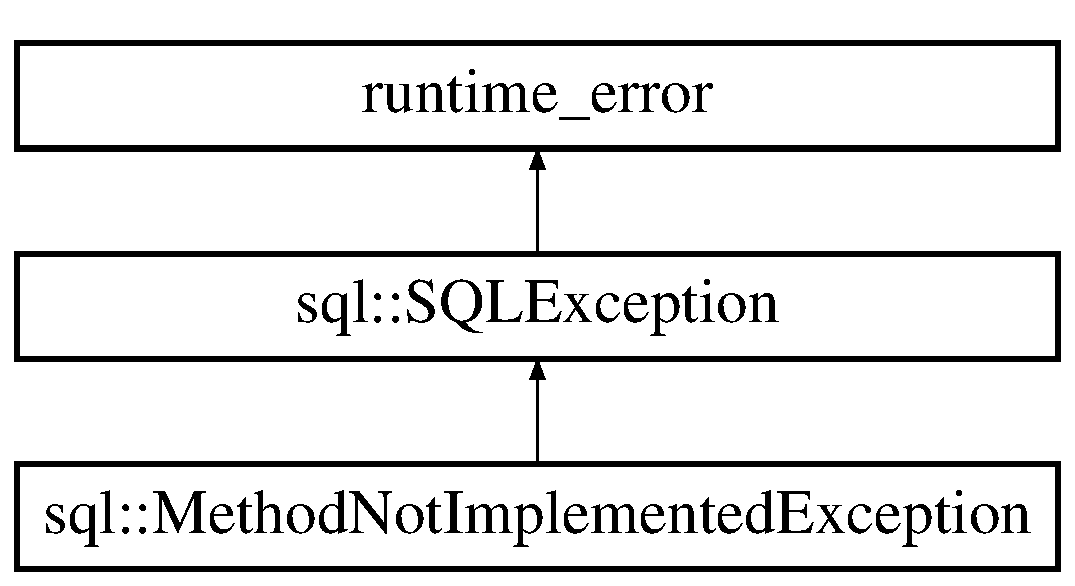
\includegraphics[height=3.000000cm]{structsql_1_1_method_not_implemented_exception}
\end{center}
\end{figure}
\subsection*{Public Member Functions}
\begin{DoxyCompactItemize}
\item 
\hypertarget{structsql_1_1_method_not_implemented_exception_a7e3e43c53ae4c0f108a262656eb534eb}{}\label{structsql_1_1_method_not_implemented_exception_a7e3e43c53ae4c0f108a262656eb534eb} 
{\bfseries Method\+Not\+Implemented\+Exception} (const \hyperlink{structsql_1_1_method_not_implemented_exception}{Method\+Not\+Implemented\+Exception} \&e)
\item 
\hypertarget{structsql_1_1_method_not_implemented_exception_aa71492d2aa8821232eeb9b9bd4c41d37}{}\label{structsql_1_1_method_not_implemented_exception_aa71492d2aa8821232eeb9b9bd4c41d37} 
{\bfseries Method\+Not\+Implemented\+Exception} (const std\+::string \&reason)
\end{DoxyCompactItemize}
\subsection*{Additional Inherited Members}


The documentation for this struct was generated from the following file\+:\begin{DoxyCompactItemize}
\item 
E\+:/projekt\+\_\+cpp\+\_\+magazyn/projekt/\+Magazyn/\+Magazyn/\+Magazyn/mysql/include/cppconn/exception.\+h\end{DoxyCompactItemize}

\hypertarget{classsql_1_1mysql_1_1_my_s_q_l___connection}{}\section{sql\+:\+:mysql\+:\+:My\+S\+Q\+L\+\_\+\+Connection Class Reference}
\label{classsql_1_1mysql_1_1_my_s_q_l___connection}\index{sql\+::mysql\+::\+My\+S\+Q\+L\+\_\+\+Connection@{sql\+::mysql\+::\+My\+S\+Q\+L\+\_\+\+Connection}}
Inheritance diagram for sql\+:\+:mysql\+:\+:My\+S\+Q\+L\+\_\+\+Connection\+:\begin{figure}[H]
\begin{center}
\leavevmode
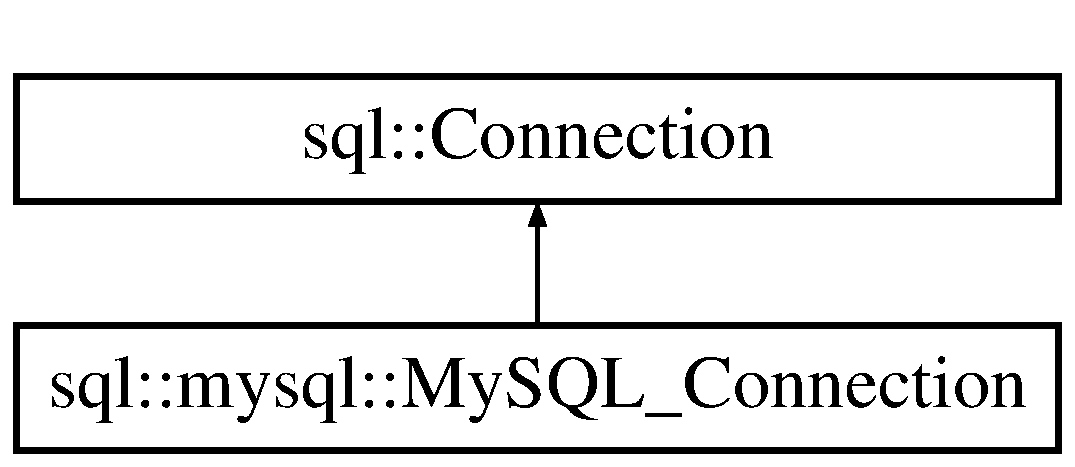
\includegraphics[height=2.000000cm]{classsql_1_1mysql_1_1_my_s_q_l___connection}
\end{center}
\end{figure}
\subsection*{Public Member Functions}
\begin{DoxyCompactItemize}
\item 
\hypertarget{classsql_1_1mysql_1_1_my_s_q_l___connection_a8b17e7794b1eb2199b63c47db273e130}{}\label{classsql_1_1mysql_1_1_my_s_q_l___connection_a8b17e7794b1eb2199b63c47db273e130} 
{\bfseries My\+S\+Q\+L\+\_\+\+Connection} (\hyperlink{classsql_1_1_driver}{Driver} $\ast$\+\_\+driver, \+::sql\+::mysql\+::\+Native\+A\+P\+I\+::\+Native\+Connection\+Wrapper \&\+\_\+proxy, const \hyperlink{classsql_1_1_s_q_l_string}{sql\+::\+S\+Q\+L\+String} \&host\+Name, const \hyperlink{classsql_1_1_s_q_l_string}{sql\+::\+S\+Q\+L\+String} \&user\+Name, const \hyperlink{classsql_1_1_s_q_l_string}{sql\+::\+S\+Q\+L\+String} \&password)
\item 
\hypertarget{classsql_1_1mysql_1_1_my_s_q_l___connection_a5462b93002e38f0462562eccf6a3c8c1}{}\label{classsql_1_1mysql_1_1_my_s_q_l___connection_a5462b93002e38f0462562eccf6a3c8c1} 
{\bfseries My\+S\+Q\+L\+\_\+\+Connection} (\hyperlink{classsql_1_1_driver}{Driver} $\ast$\+\_\+driver, \+::sql\+::mysql\+::\+Native\+A\+P\+I\+::\+Native\+Connection\+Wrapper \&\+\_\+proxy, std\+::map$<$ \hyperlink{classsql_1_1_s_q_l_string}{sql\+::\+S\+Q\+L\+String}, \hyperlink{classsql_1_1_variant}{sql\+::\+Connect\+Property\+Val} $>$ \&options)
\item 
\hypertarget{classsql_1_1mysql_1_1_my_s_q_l___connection_aa792ed9b722ec4b45842872865fcc1d9}{}\label{classsql_1_1mysql_1_1_my_s_q_l___connection_aa792ed9b722ec4b45842872865fcc1d9} 
void {\bfseries clear\+Warnings} ()
\item 
\hypertarget{classsql_1_1mysql_1_1_my_s_q_l___connection_aa8d0be382f89bfe031d276a2c67bb7fb}{}\label{classsql_1_1mysql_1_1_my_s_q_l___connection_aa8d0be382f89bfe031d276a2c67bb7fb} 
void {\bfseries close} ()
\item 
\hypertarget{classsql_1_1mysql_1_1_my_s_q_l___connection_aca3dab58cd10c2bd877fadc2fa7b9b3f}{}\label{classsql_1_1mysql_1_1_my_s_q_l___connection_aca3dab58cd10c2bd877fadc2fa7b9b3f} 
void {\bfseries commit} ()
\item 
\hypertarget{classsql_1_1mysql_1_1_my_s_q_l___connection_a65dd9ce62b91f6ee7422bf6acaa6dc59}{}\label{classsql_1_1mysql_1_1_my_s_q_l___connection_a65dd9ce62b91f6ee7422bf6acaa6dc59} 
\hyperlink{classsql_1_1_statement}{sql\+::\+Statement} $\ast$ {\bfseries create\+Statement} ()
\item 
\hypertarget{classsql_1_1mysql_1_1_my_s_q_l___connection_a4ab19794fc96f0b771dc7f3a9b89d445}{}\label{classsql_1_1mysql_1_1_my_s_q_l___connection_a4ab19794fc96f0b771dc7f3a9b89d445} 
\hyperlink{classsql_1_1_s_q_l_string}{sql\+::\+S\+Q\+L\+String} {\bfseries escape\+String} (const \hyperlink{classsql_1_1_s_q_l_string}{sql\+::\+S\+Q\+L\+String} \&)
\item 
\hypertarget{classsql_1_1mysql_1_1_my_s_q_l___connection_aa8a7c0dfd9b9dd7f8c00c43fefa2f8a4}{}\label{classsql_1_1mysql_1_1_my_s_q_l___connection_aa8a7c0dfd9b9dd7f8c00c43fefa2f8a4} 
bool {\bfseries get\+Auto\+Commit} ()
\item 
\hypertarget{classsql_1_1mysql_1_1_my_s_q_l___connection_af410a283060804936031001d38f89e9b}{}\label{classsql_1_1mysql_1_1_my_s_q_l___connection_af410a283060804936031001d38f89e9b} 
\hyperlink{classsql_1_1_s_q_l_string}{sql\+::\+S\+Q\+L\+String} {\bfseries get\+Catalog} ()
\item 
\hypertarget{classsql_1_1mysql_1_1_my_s_q_l___connection_af4aaa6f7a2564e6cd7b259a24fe8f0ef}{}\label{classsql_1_1mysql_1_1_my_s_q_l___connection_af4aaa6f7a2564e6cd7b259a24fe8f0ef} 
\hyperlink{classsql_1_1_driver}{Driver} $\ast$ {\bfseries get\+Driver} ()
\item 
\hypertarget{classsql_1_1mysql_1_1_my_s_q_l___connection_a49bf51d2c4586f8f85c362a6c71cf8b6}{}\label{classsql_1_1mysql_1_1_my_s_q_l___connection_a49bf51d2c4586f8f85c362a6c71cf8b6} 
\hyperlink{classsql_1_1_s_q_l_string}{sql\+::\+S\+Q\+L\+String} {\bfseries get\+Schema} ()
\item 
\hypertarget{classsql_1_1mysql_1_1_my_s_q_l___connection_aa94814c22d27fae1f62f8a077619026c}{}\label{classsql_1_1mysql_1_1_my_s_q_l___connection_aa94814c22d27fae1f62f8a077619026c} 
\hyperlink{classsql_1_1_s_q_l_string}{sql\+::\+S\+Q\+L\+String} {\bfseries get\+Client\+Info} ()
\item 
\hypertarget{classsql_1_1mysql_1_1_my_s_q_l___connection_a0c80ccabb9723fc4e7bcbe1fac2b7cbf}{}\label{classsql_1_1mysql_1_1_my_s_q_l___connection_a0c80ccabb9723fc4e7bcbe1fac2b7cbf} 
void {\bfseries get\+Client\+Option} (const \hyperlink{classsql_1_1_s_q_l_string}{sql\+::\+S\+Q\+L\+String} \&option\+Name, void $\ast$option\+Value)
\item 
\hypertarget{classsql_1_1mysql_1_1_my_s_q_l___connection_a6aa6995181dd5acfa0c18ec7917d2d02}{}\label{classsql_1_1mysql_1_1_my_s_q_l___connection_a6aa6995181dd5acfa0c18ec7917d2d02} 
\hyperlink{classsql_1_1_s_q_l_string}{sql\+::\+S\+Q\+L\+String} {\bfseries get\+Client\+Option} (const \hyperlink{classsql_1_1_s_q_l_string}{sql\+::\+S\+Q\+L\+String} \&option\+Name)
\item 
\hypertarget{classsql_1_1mysql_1_1_my_s_q_l___connection_a5fcfd3fa9932acb64c36d49c0e264e95}{}\label{classsql_1_1mysql_1_1_my_s_q_l___connection_a5fcfd3fa9932acb64c36d49c0e264e95} 
\hyperlink{classsql_1_1_database_meta_data}{sql\+::\+Database\+Meta\+Data} $\ast$ {\bfseries get\+Meta\+Data} ()
\item 
\hypertarget{classsql_1_1mysql_1_1_my_s_q_l___connection_a556dcab3c0deb14fde548a270d9168ad}{}\label{classsql_1_1mysql_1_1_my_s_q_l___connection_a556dcab3c0deb14fde548a270d9168ad} 
enum\+\_\+transaction\+\_\+isolation {\bfseries get\+Transaction\+Isolation} ()
\item 
\hypertarget{classsql_1_1mysql_1_1_my_s_q_l___connection_a62b556bf59e83dae5bafd52cce4801a7}{}\label{classsql_1_1mysql_1_1_my_s_q_l___connection_a62b556bf59e83dae5bafd52cce4801a7} 
const \hyperlink{classsql_1_1_s_q_l_warning}{S\+Q\+L\+Warning} $\ast$ {\bfseries get\+Warnings} ()
\item 
\hypertarget{classsql_1_1mysql_1_1_my_s_q_l___connection_a00820cf65fea6a9fd9cb936a6781db33}{}\label{classsql_1_1mysql_1_1_my_s_q_l___connection_a00820cf65fea6a9fd9cb936a6781db33} 
bool {\bfseries is\+Closed} ()
\item 
\hypertarget{classsql_1_1mysql_1_1_my_s_q_l___connection_af395e4c12315d0dcf9e3a5abbcbb33e2}{}\label{classsql_1_1mysql_1_1_my_s_q_l___connection_af395e4c12315d0dcf9e3a5abbcbb33e2} 
bool {\bfseries is\+Read\+Only} ()
\item 
\hypertarget{classsql_1_1mysql_1_1_my_s_q_l___connection_a081337e746b0eabcf0a7cb136b50277b}{}\label{classsql_1_1mysql_1_1_my_s_q_l___connection_a081337e746b0eabcf0a7cb136b50277b} 
bool {\bfseries is\+Valid} ()
\item 
\hypertarget{classsql_1_1mysql_1_1_my_s_q_l___connection_a19ebafbbc4bc37958bcc93c7fa0807e9}{}\label{classsql_1_1mysql_1_1_my_s_q_l___connection_a19ebafbbc4bc37958bcc93c7fa0807e9} 
bool {\bfseries reconnect} ()
\item 
\hypertarget{classsql_1_1mysql_1_1_my_s_q_l___connection_a7242075ae362ec3fbe65194f7043abc4}{}\label{classsql_1_1mysql_1_1_my_s_q_l___connection_a7242075ae362ec3fbe65194f7043abc4} 
\hyperlink{classsql_1_1_s_q_l_string}{sql\+::\+S\+Q\+L\+String} {\bfseries native\+S\+QL} (const \hyperlink{classsql_1_1_s_q_l_string}{sql\+::\+S\+Q\+L\+String} \&sql)
\item 
\hypertarget{classsql_1_1mysql_1_1_my_s_q_l___connection_a5d4ab19b238692240183b849c84c2166}{}\label{classsql_1_1mysql_1_1_my_s_q_l___connection_a5d4ab19b238692240183b849c84c2166} 
\hyperlink{classsql_1_1_prepared_statement}{sql\+::\+Prepared\+Statement} $\ast$ {\bfseries prepare\+Statement} (const \hyperlink{classsql_1_1_s_q_l_string}{sql\+::\+S\+Q\+L\+String} \&sql)
\item 
\hypertarget{classsql_1_1mysql_1_1_my_s_q_l___connection_a4b341cf31b1fadb55fa573d5fc570de7}{}\label{classsql_1_1mysql_1_1_my_s_q_l___connection_a4b341cf31b1fadb55fa573d5fc570de7} 
\hyperlink{classsql_1_1_prepared_statement}{sql\+::\+Prepared\+Statement} $\ast$ {\bfseries prepare\+Statement} (const \hyperlink{classsql_1_1_s_q_l_string}{sql\+::\+S\+Q\+L\+String} \&sql, int auto\+Generated\+Keys)
\item 
\hypertarget{classsql_1_1mysql_1_1_my_s_q_l___connection_a02a26ce23b897f09189ddafd4b87849e}{}\label{classsql_1_1mysql_1_1_my_s_q_l___connection_a02a26ce23b897f09189ddafd4b87849e} 
\hyperlink{classsql_1_1_prepared_statement}{sql\+::\+Prepared\+Statement} $\ast$ {\bfseries prepare\+Statement} (const \hyperlink{classsql_1_1_s_q_l_string}{sql\+::\+S\+Q\+L\+String} \&sql, int column\+Indexes\mbox{[}$\,$\mbox{]})
\item 
\hypertarget{classsql_1_1mysql_1_1_my_s_q_l___connection_afcddea07aca0542a2a6e814ba1ee4bd6}{}\label{classsql_1_1mysql_1_1_my_s_q_l___connection_afcddea07aca0542a2a6e814ba1ee4bd6} 
\hyperlink{classsql_1_1_prepared_statement}{sql\+::\+Prepared\+Statement} $\ast$ {\bfseries prepare\+Statement} (const \hyperlink{classsql_1_1_s_q_l_string}{sql\+::\+S\+Q\+L\+String} \&sql, int result\+Set\+Type, int result\+Set\+Concurrency)
\item 
\hypertarget{classsql_1_1mysql_1_1_my_s_q_l___connection_a156ab360753b8b1ca11682422d9914b3}{}\label{classsql_1_1mysql_1_1_my_s_q_l___connection_a156ab360753b8b1ca11682422d9914b3} 
\hyperlink{classsql_1_1_prepared_statement}{sql\+::\+Prepared\+Statement} $\ast$ {\bfseries prepare\+Statement} (const \hyperlink{classsql_1_1_s_q_l_string}{sql\+::\+S\+Q\+L\+String} \&sql, int result\+Set\+Type, int result\+Set\+Concurrency, int result\+Set\+Holdability)
\item 
\hypertarget{classsql_1_1mysql_1_1_my_s_q_l___connection_a27a07ce9777574a0592fe6f8834e082f}{}\label{classsql_1_1mysql_1_1_my_s_q_l___connection_a27a07ce9777574a0592fe6f8834e082f} 
\hyperlink{classsql_1_1_prepared_statement}{sql\+::\+Prepared\+Statement} $\ast$ {\bfseries prepare\+Statement} (const \hyperlink{classsql_1_1_s_q_l_string}{sql\+::\+S\+Q\+L\+String} \&sql, \hyperlink{classsql_1_1_s_q_l_string}{sql\+::\+S\+Q\+L\+String} column\+Names\mbox{[}$\,$\mbox{]})
\item 
\hypertarget{classsql_1_1mysql_1_1_my_s_q_l___connection_af85e740e1d7cc9f16d357afdd9f4419d}{}\label{classsql_1_1mysql_1_1_my_s_q_l___connection_af85e740e1d7cc9f16d357afdd9f4419d} 
void {\bfseries release\+Savepoint} (\hyperlink{classsql_1_1_savepoint}{Savepoint} $\ast$savepoint)
\item 
\hypertarget{classsql_1_1mysql_1_1_my_s_q_l___connection_a30102a74e65a62cff9c36ce77a8c7f44}{}\label{classsql_1_1mysql_1_1_my_s_q_l___connection_a30102a74e65a62cff9c36ce77a8c7f44} 
void {\bfseries rollback} ()
\item 
\hypertarget{classsql_1_1mysql_1_1_my_s_q_l___connection_a64fc3a6f403a19fee712142141a07ef4}{}\label{classsql_1_1mysql_1_1_my_s_q_l___connection_a64fc3a6f403a19fee712142141a07ef4} 
void {\bfseries rollback} (\hyperlink{classsql_1_1_savepoint}{Savepoint} $\ast$savepoint)
\item 
\hypertarget{classsql_1_1mysql_1_1_my_s_q_l___connection_a66dd8515ee9ccfe186fc1d2b597f220f}{}\label{classsql_1_1mysql_1_1_my_s_q_l___connection_a66dd8515ee9ccfe186fc1d2b597f220f} 
void {\bfseries set\+Auto\+Commit} (bool auto\+Commit)
\item 
\hypertarget{classsql_1_1mysql_1_1_my_s_q_l___connection_a85487982563f163064269bbe072bf2a0}{}\label{classsql_1_1mysql_1_1_my_s_q_l___connection_a85487982563f163064269bbe072bf2a0} 
void {\bfseries set\+Catalog} (const \hyperlink{classsql_1_1_s_q_l_string}{sql\+::\+S\+Q\+L\+String} \&catalog)
\item 
\hypertarget{classsql_1_1mysql_1_1_my_s_q_l___connection_ae9c04f366688e047e898487bc6fd6e1b}{}\label{classsql_1_1mysql_1_1_my_s_q_l___connection_ae9c04f366688e047e898487bc6fd6e1b} 
void {\bfseries set\+Schema} (const \hyperlink{classsql_1_1_s_q_l_string}{sql\+::\+S\+Q\+L\+String} \&catalog)
\item 
\hypertarget{classsql_1_1mysql_1_1_my_s_q_l___connection_a146973ddeaf89e344b719cefb09c55ad}{}\label{classsql_1_1mysql_1_1_my_s_q_l___connection_a146973ddeaf89e344b719cefb09c55ad} 
\hyperlink{classsql_1_1_connection}{sql\+::\+Connection} $\ast$ {\bfseries set\+Client\+Option} (const \hyperlink{classsql_1_1_s_q_l_string}{sql\+::\+S\+Q\+L\+String} \&option\+Name, const void $\ast$option\+Value)
\item 
\hypertarget{classsql_1_1mysql_1_1_my_s_q_l___connection_a2e01fff22d660d797501ac29e9a436e7}{}\label{classsql_1_1mysql_1_1_my_s_q_l___connection_a2e01fff22d660d797501ac29e9a436e7} 
\hyperlink{classsql_1_1_connection}{sql\+::\+Connection} $\ast$ {\bfseries set\+Client\+Option} (const \hyperlink{classsql_1_1_s_q_l_string}{sql\+::\+S\+Q\+L\+String} \&option\+Name, const \hyperlink{classsql_1_1_s_q_l_string}{sql\+::\+S\+Q\+L\+String} \&option\+Value)
\item 
\hypertarget{classsql_1_1mysql_1_1_my_s_q_l___connection_a4703a47ce23ba73ec2fadfc680b2e868}{}\label{classsql_1_1mysql_1_1_my_s_q_l___connection_a4703a47ce23ba73ec2fadfc680b2e868} 
void {\bfseries set\+Holdability} (int holdability)
\item 
\hypertarget{classsql_1_1mysql_1_1_my_s_q_l___connection_ac4bafbedfb801fa73694ddbfca4a95c6}{}\label{classsql_1_1mysql_1_1_my_s_q_l___connection_ac4bafbedfb801fa73694ddbfca4a95c6} 
void {\bfseries set\+Read\+Only} (bool read\+Only)
\item 
\hypertarget{classsql_1_1mysql_1_1_my_s_q_l___connection_afca8998459c9f06788b3ed3be25b81de}{}\label{classsql_1_1mysql_1_1_my_s_q_l___connection_afca8998459c9f06788b3ed3be25b81de} 
\hyperlink{classsql_1_1_savepoint}{sql\+::\+Savepoint} $\ast$ {\bfseries set\+Savepoint} ()
\item 
\hypertarget{classsql_1_1mysql_1_1_my_s_q_l___connection_a2d0045db252b83fd0222e716f9bfc71d}{}\label{classsql_1_1mysql_1_1_my_s_q_l___connection_a2d0045db252b83fd0222e716f9bfc71d} 
\hyperlink{classsql_1_1_savepoint}{sql\+::\+Savepoint} $\ast$ {\bfseries set\+Savepoint} (const \hyperlink{classsql_1_1_s_q_l_string}{sql\+::\+S\+Q\+L\+String} \&name)
\item 
\hypertarget{classsql_1_1mysql_1_1_my_s_q_l___connection_a50c5f85205c2333804ee503778ed05b0}{}\label{classsql_1_1mysql_1_1_my_s_q_l___connection_a50c5f85205c2333804ee503778ed05b0} 
void {\bfseries set\+Transaction\+Isolation} (enum\+\_\+transaction\+\_\+isolation level)
\item 
\hypertarget{classsql_1_1mysql_1_1_my_s_q_l___connection_ae35fdfcee5de39dc2ec759bc5b8145be}{}\label{classsql_1_1mysql_1_1_my_s_q_l___connection_ae35fdfcee5de39dc2ec759bc5b8145be} 
virtual \hyperlink{classsql_1_1_s_q_l_string}{sql\+::\+S\+Q\+L\+String} {\bfseries get\+Session\+Variable} (const \hyperlink{classsql_1_1_s_q_l_string}{sql\+::\+S\+Q\+L\+String} \&varname)
\item 
\hypertarget{classsql_1_1mysql_1_1_my_s_q_l___connection_a5e3eb3eed3d7092c9d03efd7d52629c2}{}\label{classsql_1_1mysql_1_1_my_s_q_l___connection_a5e3eb3eed3d7092c9d03efd7d52629c2} 
virtual void {\bfseries set\+Session\+Variable} (const \hyperlink{classsql_1_1_s_q_l_string}{sql\+::\+S\+Q\+L\+String} \&varname, const \hyperlink{classsql_1_1_s_q_l_string}{sql\+::\+S\+Q\+L\+String} \&value)
\item 
\hypertarget{classsql_1_1mysql_1_1_my_s_q_l___connection_ad8a42ed4da0fb3810a7624cc969d7ced}{}\label{classsql_1_1mysql_1_1_my_s_q_l___connection_ad8a42ed4da0fb3810a7624cc969d7ced} 
virtual void {\bfseries set\+Session\+Variable} (const \hyperlink{classsql_1_1_s_q_l_string}{sql\+::\+S\+Q\+L\+String} \&varname, unsigned int value)
\item 
\hypertarget{classsql_1_1mysql_1_1_my_s_q_l___connection_a31744f8fd6beaa9c488f947962c1bae6}{}\label{classsql_1_1mysql_1_1_my_s_q_l___connection_a31744f8fd6beaa9c488f947962c1bae6} 
virtual \hyperlink{classsql_1_1_s_q_l_string}{sql\+::\+S\+Q\+L\+String} {\bfseries get\+Last\+Statement\+Info} ()
\end{DoxyCompactItemize}
\subsection*{Private Member Functions}
\begin{DoxyCompactItemize}
\item 
\hypertarget{classsql_1_1mysql_1_1_my_s_q_l___connection_a99bbbb206d737a3c2a098f9005e24d6a}{}\label{classsql_1_1mysql_1_1_my_s_q_l___connection_a99bbbb206d737a3c2a098f9005e24d6a} 
My\+S\+Q\+L\+\_\+\+Statement $\ast$ {\bfseries create\+Service\+Stmt} ()
\item 
\hypertarget{classsql_1_1mysql_1_1_my_s_q_l___connection_a87aae788d1083b16d49071dbae5aeb42}{}\label{classsql_1_1mysql_1_1_my_s_q_l___connection_a87aae788d1083b16d49071dbae5aeb42} 
void {\bfseries check\+Closed} ()
\item 
\hypertarget{classsql_1_1mysql_1_1_my_s_q_l___connection_a627c6c2e541187545eeeae73f78638c9}{}\label{classsql_1_1mysql_1_1_my_s_q_l___connection_a627c6c2e541187545eeeae73f78638c9} 
void {\bfseries init} (std\+::map$<$ \hyperlink{classsql_1_1_s_q_l_string}{sql\+::\+S\+Q\+L\+String}, \hyperlink{classsql_1_1_variant}{sql\+::\+Connect\+Property\+Val} $>$ \&properties)
\item 
\hypertarget{classsql_1_1mysql_1_1_my_s_q_l___connection_ad0ef40dd00878160834850df68a1efc8}{}\label{classsql_1_1mysql_1_1_my_s_q_l___connection_ad0ef40dd00878160834850df68a1efc8} 
{\bfseries My\+S\+Q\+L\+\_\+\+Connection} (const \hyperlink{classsql_1_1mysql_1_1_my_s_q_l___connection}{My\+S\+Q\+L\+\_\+\+Connection} \&)
\item 
\hypertarget{classsql_1_1mysql_1_1_my_s_q_l___connection_a1973c5e0c52e0f5fa602a166a7d814fd}{}\label{classsql_1_1mysql_1_1_my_s_q_l___connection_a1973c5e0c52e0f5fa602a166a7d814fd} 
void {\bfseries operator=} (\hyperlink{classsql_1_1mysql_1_1_my_s_q_l___connection}{My\+S\+Q\+L\+\_\+\+Connection} \&)
\end{DoxyCompactItemize}
\subsection*{Private Attributes}
\begin{DoxyCompactItemize}
\item 
\hypertarget{classsql_1_1mysql_1_1_my_s_q_l___connection_a02c7eca4eb55f6ddadf2c81419d8faf2}{}\label{classsql_1_1mysql_1_1_my_s_q_l___connection_a02c7eca4eb55f6ddadf2c81419d8faf2} 
\hyperlink{classsql_1_1_driver}{Driver} $\ast$ {\bfseries driver}
\item 
\hypertarget{classsql_1_1mysql_1_1_my_s_q_l___connection_a4e5e011271ee687e7c42c55716f99826}{}\label{classsql_1_1mysql_1_1_my_s_q_l___connection_a4e5e011271ee687e7c42c55716f99826} 
boost\+::shared\+\_\+ptr$<$ Native\+A\+P\+I\+::\+Native\+Connection\+Wrapper $>$ {\bfseries proxy}
\item 
\hypertarget{classsql_1_1mysql_1_1_my_s_q_l___connection_a5a88e82b22a22f2f0c46f519ceff8752}{}\label{classsql_1_1mysql_1_1_my_s_q_l___connection_a5a88e82b22a22f2f0c46f519ceff8752} 
boost\+::scoped\+\_\+ptr$<$ \+::sql\+::mysql\+::\+My\+S\+Q\+L\+\_\+\+Statement $>$ {\bfseries service}
\item 
\hypertarget{classsql_1_1mysql_1_1_my_s_q_l___connection_a4fed30f045e178b5eb5baeb2ee1c7129}{}\label{classsql_1_1mysql_1_1_my_s_q_l___connection_a4fed30f045e178b5eb5baeb2ee1c7129} 
boost\+::scoped\+\_\+ptr$<$ \+::sql\+::mysql\+::\+My\+S\+Q\+L\+\_\+\+Connection\+Data $>$ {\bfseries intern}
\end{DoxyCompactItemize}


The documentation for this class was generated from the following file\+:\begin{DoxyCompactItemize}
\item 
E\+:/projekt\+\_\+cpp\+\_\+magazyn/projekt/\+Magazyn/\+Magazyn/\+Magazyn/mysql/include/mysql\+\_\+connection.\+h\end{DoxyCompactItemize}

\hypertarget{classsql_1_1mysql_1_1_my_s_q_l___driver}{}\section{sql\+:\+:mysql\+:\+:My\+S\+Q\+L\+\_\+\+Driver Class Reference}
\label{classsql_1_1mysql_1_1_my_s_q_l___driver}\index{sql\+::mysql\+::\+My\+S\+Q\+L\+\_\+\+Driver@{sql\+::mysql\+::\+My\+S\+Q\+L\+\_\+\+Driver}}
Inheritance diagram for sql\+:\+:mysql\+:\+:My\+S\+Q\+L\+\_\+\+Driver\+:\begin{figure}[H]
\begin{center}
\leavevmode
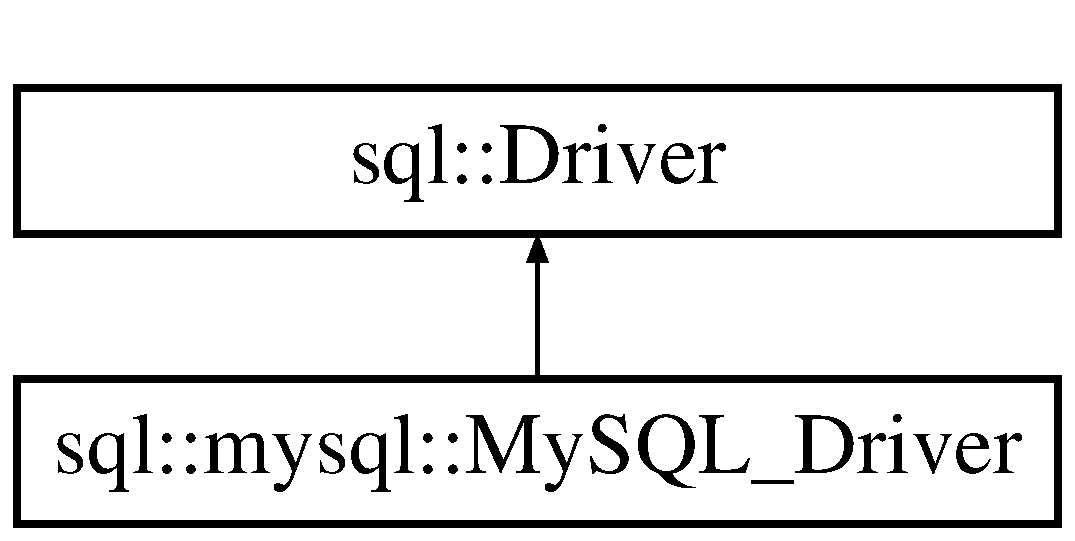
\includegraphics[height=2.000000cm]{classsql_1_1mysql_1_1_my_s_q_l___driver}
\end{center}
\end{figure}
\subsection*{Public Member Functions}
\begin{DoxyCompactItemize}
\item 
\hypertarget{classsql_1_1mysql_1_1_my_s_q_l___driver_a9fb0b703cfe41e14c9119a5445eb5abd}{}\label{classsql_1_1mysql_1_1_my_s_q_l___driver_a9fb0b703cfe41e14c9119a5445eb5abd} 
{\bfseries My\+S\+Q\+L\+\_\+\+Driver} (const \+::\hyperlink{classsql_1_1_s_q_l_string}{sql\+::\+S\+Q\+L\+String} \&client\+Lib)
\item 
\hypertarget{classsql_1_1mysql_1_1_my_s_q_l___driver_aa04c5abeb14fdcc975b8102ea3b50da2}{}\label{classsql_1_1mysql_1_1_my_s_q_l___driver_aa04c5abeb14fdcc975b8102ea3b50da2} 
\hyperlink{classsql_1_1_connection}{sql\+::\+Connection} $\ast$ {\bfseries connect} (const \hyperlink{classsql_1_1_s_q_l_string}{sql\+::\+S\+Q\+L\+String} \&host\+Name, const \hyperlink{classsql_1_1_s_q_l_string}{sql\+::\+S\+Q\+L\+String} \&user\+Name, const \hyperlink{classsql_1_1_s_q_l_string}{sql\+::\+S\+Q\+L\+String} \&password)
\item 
\hypertarget{classsql_1_1mysql_1_1_my_s_q_l___driver_a3115896b0002e58542b671c54cbf4fd0}{}\label{classsql_1_1mysql_1_1_my_s_q_l___driver_a3115896b0002e58542b671c54cbf4fd0} 
\hyperlink{classsql_1_1_connection}{sql\+::\+Connection} $\ast$ {\bfseries connect} (sql\+::\+Connect\+Options\+Map \&options)
\item 
\hypertarget{classsql_1_1mysql_1_1_my_s_q_l___driver_a18ad292b17b6e55f42aac77f55fcc60f}{}\label{classsql_1_1mysql_1_1_my_s_q_l___driver_a18ad292b17b6e55f42aac77f55fcc60f} 
int {\bfseries get\+Major\+Version} ()
\item 
\hypertarget{classsql_1_1mysql_1_1_my_s_q_l___driver_acb105dd8eda7a255f92dde830dbf9379}{}\label{classsql_1_1mysql_1_1_my_s_q_l___driver_acb105dd8eda7a255f92dde830dbf9379} 
int {\bfseries get\+Minor\+Version} ()
\item 
\hypertarget{classsql_1_1mysql_1_1_my_s_q_l___driver_accfffb055fedaae4f29f0df9c017c229}{}\label{classsql_1_1mysql_1_1_my_s_q_l___driver_accfffb055fedaae4f29f0df9c017c229} 
int {\bfseries get\+Patch\+Version} ()
\item 
\hypertarget{classsql_1_1mysql_1_1_my_s_q_l___driver_a79a72cba4218175ed7044b34619eb1f6}{}\label{classsql_1_1mysql_1_1_my_s_q_l___driver_a79a72cba4218175ed7044b34619eb1f6} 
const \hyperlink{classsql_1_1_s_q_l_string}{sql\+::\+S\+Q\+L\+String} \& {\bfseries get\+Name} ()
\item 
\hypertarget{classsql_1_1mysql_1_1_my_s_q_l___driver_a36f80c3744c40034a2cbad72619021c6}{}\label{classsql_1_1mysql_1_1_my_s_q_l___driver_a36f80c3744c40034a2cbad72619021c6} 
void {\bfseries thread\+Init} ()
\item 
\hypertarget{classsql_1_1mysql_1_1_my_s_q_l___driver_adcf58599e9e55017d00057029b910a24}{}\label{classsql_1_1mysql_1_1_my_s_q_l___driver_adcf58599e9e55017d00057029b910a24} 
void {\bfseries thread\+End} ()
\end{DoxyCompactItemize}
\subsection*{Private Member Functions}
\begin{DoxyCompactItemize}
\item 
\hypertarget{classsql_1_1mysql_1_1_my_s_q_l___driver_a05b8667fbe350ca63151f9d3ca7e6384}{}\label{classsql_1_1mysql_1_1_my_s_q_l___driver_a05b8667fbe350ca63151f9d3ca7e6384} 
{\bfseries My\+S\+Q\+L\+\_\+\+Driver} (const \hyperlink{classsql_1_1mysql_1_1_my_s_q_l___driver}{My\+S\+Q\+L\+\_\+\+Driver} \&)
\item 
\hypertarget{classsql_1_1mysql_1_1_my_s_q_l___driver_a1e2751b67245d1d307d5f3ed31620434}{}\label{classsql_1_1mysql_1_1_my_s_q_l___driver_a1e2751b67245d1d307d5f3ed31620434} 
void {\bfseries operator=} (\hyperlink{classsql_1_1mysql_1_1_my_s_q_l___driver}{My\+S\+Q\+L\+\_\+\+Driver} \&)
\end{DoxyCompactItemize}
\subsection*{Private Attributes}
\begin{DoxyCompactItemize}
\item 
\hypertarget{classsql_1_1mysql_1_1_my_s_q_l___driver_a25d9763be9bb3b0b1364caf83dc03e38}{}\label{classsql_1_1mysql_1_1_my_s_q_l___driver_a25d9763be9bb3b0b1364caf83dc03e38} 
boost\+::scoped\+\_\+ptr$<$ \+::sql\+::mysql\+::\+Native\+A\+P\+I\+::\+Native\+Driver\+Wrapper $>$ {\bfseries proxy}
\end{DoxyCompactItemize}


The documentation for this class was generated from the following file\+:\begin{DoxyCompactItemize}
\item 
E\+:/projekt\+\_\+cpp\+\_\+magazyn/projekt/\+Magazyn/\+Magazyn/\+Magazyn/mysql/include/mysql\+\_\+driver.\+h\end{DoxyCompactItemize}

\hypertarget{classsql_1_1mysql_1_1_my_s_q_l___savepoint}{}\section{sql\+:\+:mysql\+:\+:My\+S\+Q\+L\+\_\+\+Savepoint Class Reference}
\label{classsql_1_1mysql_1_1_my_s_q_l___savepoint}\index{sql\+::mysql\+::\+My\+S\+Q\+L\+\_\+\+Savepoint@{sql\+::mysql\+::\+My\+S\+Q\+L\+\_\+\+Savepoint}}
Inheritance diagram for sql\+:\+:mysql\+:\+:My\+S\+Q\+L\+\_\+\+Savepoint\+:\begin{figure}[H]
\begin{center}
\leavevmode
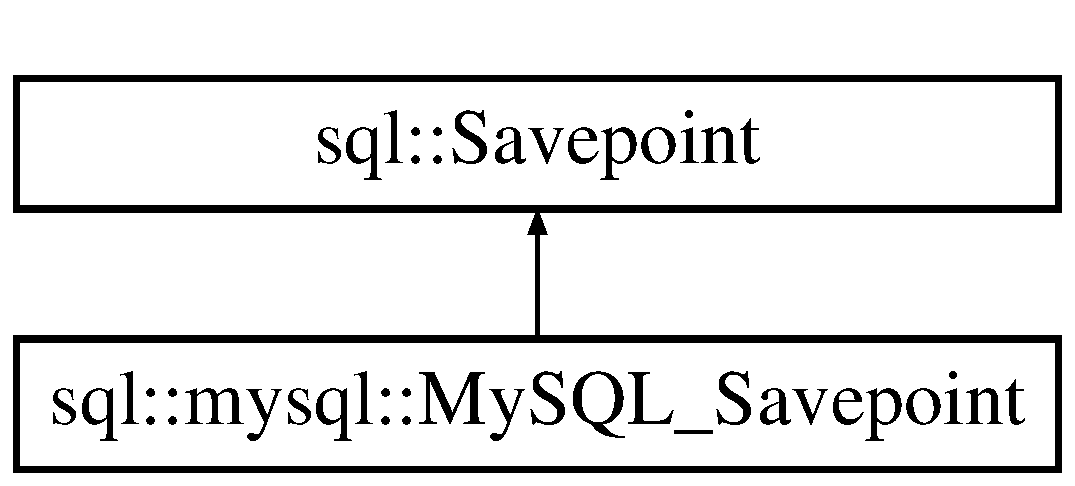
\includegraphics[height=2.000000cm]{classsql_1_1mysql_1_1_my_s_q_l___savepoint}
\end{center}
\end{figure}
\subsection*{Public Member Functions}
\begin{DoxyCompactItemize}
\item 
\hypertarget{classsql_1_1mysql_1_1_my_s_q_l___savepoint_a864a5455837699c737623060010dd7b5}{}\label{classsql_1_1mysql_1_1_my_s_q_l___savepoint_a864a5455837699c737623060010dd7b5} 
{\bfseries My\+S\+Q\+L\+\_\+\+Savepoint} (const \hyperlink{classsql_1_1_s_q_l_string}{sql\+::\+S\+Q\+L\+String} \&savepoint)
\item 
\hypertarget{classsql_1_1mysql_1_1_my_s_q_l___savepoint_a0fb4031dfa691e3f2453c2d9eff5ea09}{}\label{classsql_1_1mysql_1_1_my_s_q_l___savepoint_a0fb4031dfa691e3f2453c2d9eff5ea09} 
int {\bfseries get\+Savepoint\+Id} ()
\item 
\hypertarget{classsql_1_1mysql_1_1_my_s_q_l___savepoint_a7c2aeca2f1c37da2ae0fe213eb9e6b40}{}\label{classsql_1_1mysql_1_1_my_s_q_l___savepoint_a7c2aeca2f1c37da2ae0fe213eb9e6b40} 
\hyperlink{classsql_1_1_s_q_l_string}{sql\+::\+S\+Q\+L\+String} {\bfseries get\+Savepoint\+Name} ()
\end{DoxyCompactItemize}
\subsection*{Private Member Functions}
\begin{DoxyCompactItemize}
\item 
\hypertarget{classsql_1_1mysql_1_1_my_s_q_l___savepoint_a5d22419f41050d85a471221aa2ab1e77}{}\label{classsql_1_1mysql_1_1_my_s_q_l___savepoint_a5d22419f41050d85a471221aa2ab1e77} 
{\bfseries My\+S\+Q\+L\+\_\+\+Savepoint} (const \hyperlink{classsql_1_1mysql_1_1_my_s_q_l___savepoint}{My\+S\+Q\+L\+\_\+\+Savepoint} \&)
\item 
\hypertarget{classsql_1_1mysql_1_1_my_s_q_l___savepoint_a5fe990219bc8761d47233c95867b52c4}{}\label{classsql_1_1mysql_1_1_my_s_q_l___savepoint_a5fe990219bc8761d47233c95867b52c4} 
void {\bfseries operator=} (\hyperlink{classsql_1_1mysql_1_1_my_s_q_l___savepoint}{My\+S\+Q\+L\+\_\+\+Savepoint} \&)
\end{DoxyCompactItemize}
\subsection*{Private Attributes}
\begin{DoxyCompactItemize}
\item 
\hypertarget{classsql_1_1mysql_1_1_my_s_q_l___savepoint_aa1e58ade85d613b0a7e577470111b6e7}{}\label{classsql_1_1mysql_1_1_my_s_q_l___savepoint_aa1e58ade85d613b0a7e577470111b6e7} 
\hyperlink{classsql_1_1_s_q_l_string}{sql\+::\+S\+Q\+L\+String} {\bfseries name}
\end{DoxyCompactItemize}


The documentation for this class was generated from the following file\+:\begin{DoxyCompactItemize}
\item 
E\+:/projekt\+\_\+cpp\+\_\+magazyn/projekt/\+Magazyn/\+Magazyn/\+Magazyn/mysql/include/mysql\+\_\+connection.\+h\end{DoxyCompactItemize}

\hypertarget{structsql_1_1_non_scrollable_exception}{}\section{sql\+:\+:Non\+Scrollable\+Exception Struct Reference}
\label{structsql_1_1_non_scrollable_exception}\index{sql\+::\+Non\+Scrollable\+Exception@{sql\+::\+Non\+Scrollable\+Exception}}
Inheritance diagram for sql\+:\+:Non\+Scrollable\+Exception\+:\begin{figure}[H]
\begin{center}
\leavevmode
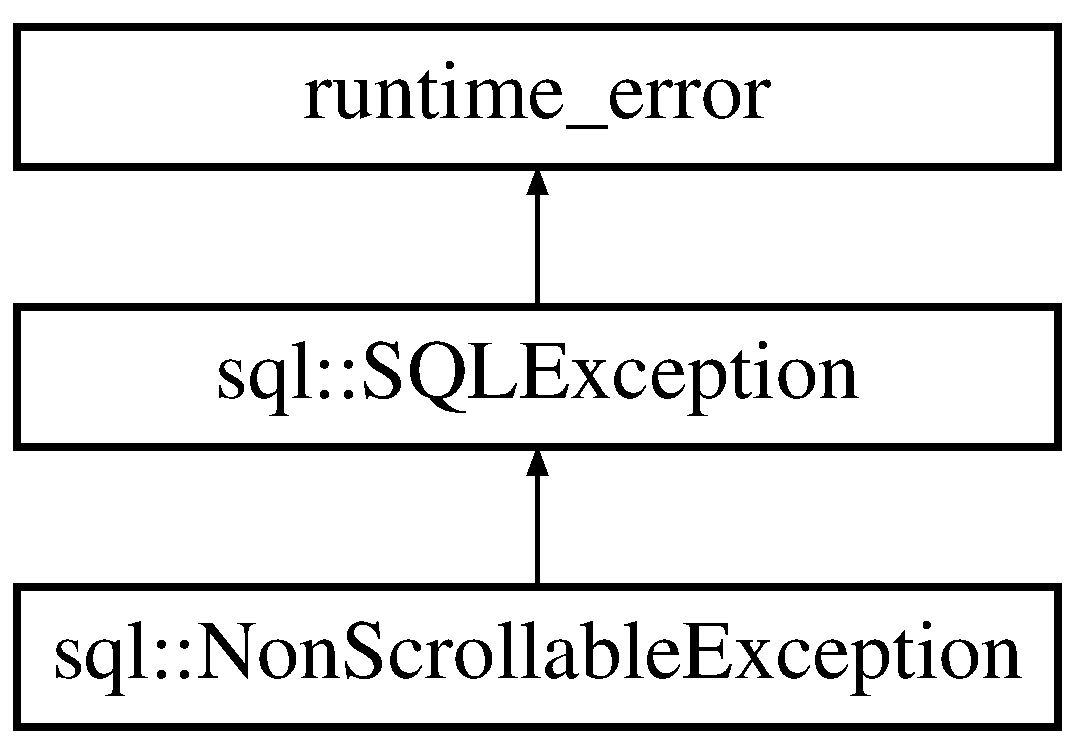
\includegraphics[height=3.000000cm]{structsql_1_1_non_scrollable_exception}
\end{center}
\end{figure}
\subsection*{Public Member Functions}
\begin{DoxyCompactItemize}
\item 
\hypertarget{structsql_1_1_non_scrollable_exception_a1f863bfa3628a5ddaca62698a5ccab72}{}\label{structsql_1_1_non_scrollable_exception_a1f863bfa3628a5ddaca62698a5ccab72} 
{\bfseries Non\+Scrollable\+Exception} (const \hyperlink{structsql_1_1_non_scrollable_exception}{Non\+Scrollable\+Exception} \&e)
\item 
\hypertarget{structsql_1_1_non_scrollable_exception_aac07e20cf83068adcee940c28dd3de72}{}\label{structsql_1_1_non_scrollable_exception_aac07e20cf83068adcee940c28dd3de72} 
{\bfseries Non\+Scrollable\+Exception} (const std\+::string \&reason)
\end{DoxyCompactItemize}
\subsection*{Additional Inherited Members}


The documentation for this struct was generated from the following file\+:\begin{DoxyCompactItemize}
\item 
E\+:/projekt\+\_\+cpp\+\_\+magazyn/projekt/\+Magazyn/\+Magazyn/\+Magazyn/mysql/include/cppconn/exception.\+h\end{DoxyCompactItemize}

\hypertarget{classsql_1_1_parameter_meta_data}{}\section{sql\+:\+:Parameter\+Meta\+Data Class Reference}
\label{classsql_1_1_parameter_meta_data}\index{sql\+::\+Parameter\+Meta\+Data@{sql\+::\+Parameter\+Meta\+Data}}
\subsection*{Public Types}
\begin{DoxyCompactItemize}
\item 
\hypertarget{classsql_1_1_parameter_meta_data_ae0ffcd0552843910d5b6e0200740805e}{}\label{classsql_1_1_parameter_meta_data_ae0ffcd0552843910d5b6e0200740805e} 
enum \{ {\bfseries parameter\+Mode\+In}, 
{\bfseries parameter\+Mode\+In\+Out}, 
{\bfseries parameter\+Mode\+Out}, 
{\bfseries parameter\+Mode\+Unknown}
 \}
\item 
\hypertarget{classsql_1_1_parameter_meta_data_aad2c73029b4d51ee6f27890c213ab425}{}\label{classsql_1_1_parameter_meta_data_aad2c73029b4d51ee6f27890c213ab425} 
enum \{ {\bfseries parameter\+No\+Nulls}, 
{\bfseries parameter\+Nullable}, 
{\bfseries parameter\+Nullable\+Unknown}
 \}
\end{DoxyCompactItemize}
\subsection*{Public Member Functions}
\begin{DoxyCompactItemize}
\item 
\hypertarget{classsql_1_1_parameter_meta_data_a4eac0bdf826073bab398b6c92a53b7fe}{}\label{classsql_1_1_parameter_meta_data_a4eac0bdf826073bab398b6c92a53b7fe} 
virtual \hyperlink{classsql_1_1_s_q_l_string}{sql\+::\+S\+Q\+L\+String} {\bfseries get\+Parameter\+Class\+Name} (unsigned int param)=0
\item 
\hypertarget{classsql_1_1_parameter_meta_data_a76300959d4703649ea996691ec9ddc70}{}\label{classsql_1_1_parameter_meta_data_a76300959d4703649ea996691ec9ddc70} 
virtual int {\bfseries get\+Parameter\+Count} ()=0
\item 
\hypertarget{classsql_1_1_parameter_meta_data_ab46c3024b12b4b7a75b81d32340bc53b}{}\label{classsql_1_1_parameter_meta_data_ab46c3024b12b4b7a75b81d32340bc53b} 
virtual int {\bfseries get\+Parameter\+Mode} (unsigned int param)=0
\item 
\hypertarget{classsql_1_1_parameter_meta_data_a604aefdf3399674c54548ffd6d09dbd7}{}\label{classsql_1_1_parameter_meta_data_a604aefdf3399674c54548ffd6d09dbd7} 
virtual int {\bfseries get\+Parameter\+Type} (unsigned int param)=0
\item 
\hypertarget{classsql_1_1_parameter_meta_data_ae2dce4bf0b8a3e5194406f7d7d07eb88}{}\label{classsql_1_1_parameter_meta_data_ae2dce4bf0b8a3e5194406f7d7d07eb88} 
virtual \hyperlink{classsql_1_1_s_q_l_string}{sql\+::\+S\+Q\+L\+String} {\bfseries get\+Parameter\+Type\+Name} (unsigned int param)=0
\item 
\hypertarget{classsql_1_1_parameter_meta_data_a85a283b336695e7518cb35836b81cd6b}{}\label{classsql_1_1_parameter_meta_data_a85a283b336695e7518cb35836b81cd6b} 
virtual int {\bfseries get\+Precision} (unsigned int param)=0
\item 
\hypertarget{classsql_1_1_parameter_meta_data_aea9fa32949a6c4ccf6ef438d0e18fd2c}{}\label{classsql_1_1_parameter_meta_data_aea9fa32949a6c4ccf6ef438d0e18fd2c} 
virtual int {\bfseries get\+Scale} (unsigned int param)=0
\item 
\hypertarget{classsql_1_1_parameter_meta_data_aea4cfff3a14bc4b5a7e51f97ee7f1c56}{}\label{classsql_1_1_parameter_meta_data_aea4cfff3a14bc4b5a7e51f97ee7f1c56} 
virtual int {\bfseries is\+Nullable} (unsigned int param)=0
\item 
\hypertarget{classsql_1_1_parameter_meta_data_a1a6ee69d7780d6747cf8ee873b272f6a}{}\label{classsql_1_1_parameter_meta_data_a1a6ee69d7780d6747cf8ee873b272f6a} 
virtual bool {\bfseries is\+Signed} (unsigned int param)=0
\end{DoxyCompactItemize}


The documentation for this class was generated from the following file\+:\begin{DoxyCompactItemize}
\item 
E\+:/projekt\+\_\+cpp\+\_\+magazyn/projekt/\+Magazyn/\+Magazyn/\+Magazyn/mysql/include/cppconn/parameter\+\_\+metadata.\+h\end{DoxyCompactItemize}

\hypertarget{classsql_1_1_prepared_statement}{}\section{sql\+:\+:Prepared\+Statement Class Reference}
\label{classsql_1_1_prepared_statement}\index{sql\+::\+Prepared\+Statement@{sql\+::\+Prepared\+Statement}}
Inheritance diagram for sql\+:\+:Prepared\+Statement\+:\begin{figure}[H]
\begin{center}
\leavevmode
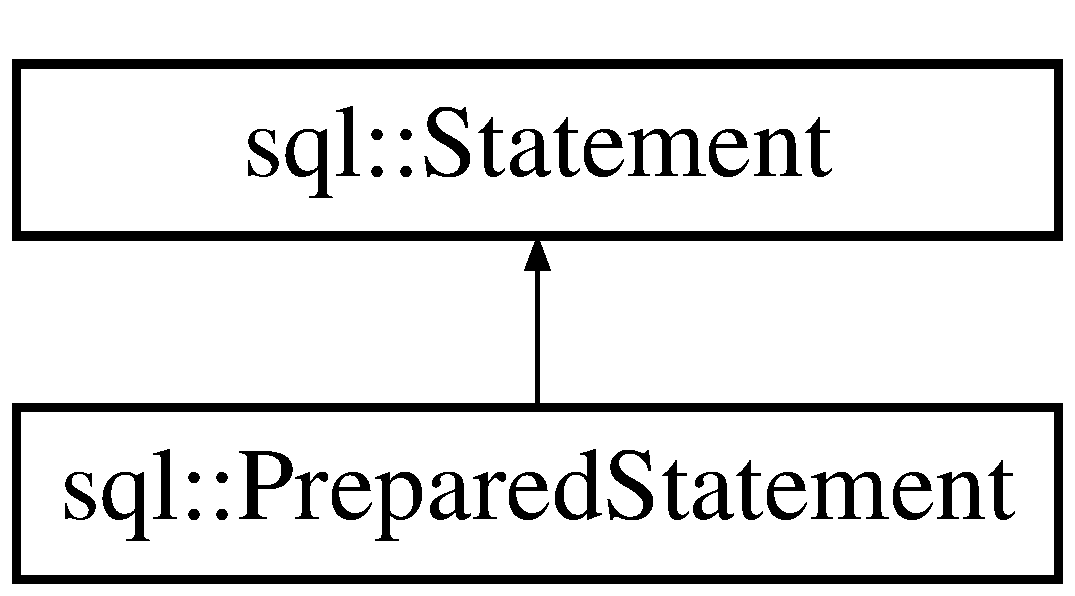
\includegraphics[height=2.000000cm]{classsql_1_1_prepared_statement}
\end{center}
\end{figure}
\subsection*{Public Member Functions}
\begin{DoxyCompactItemize}
\item 
\hypertarget{classsql_1_1_prepared_statement_ab9cb930a742cd46d3c4f7fb6be0ff4bb}{}\label{classsql_1_1_prepared_statement_ab9cb930a742cd46d3c4f7fb6be0ff4bb} 
virtual void {\bfseries clear\+Parameters} ()=0
\item 
\hypertarget{classsql_1_1_prepared_statement_a34cf6877fda80d5c1d4298c015d0ea20}{}\label{classsql_1_1_prepared_statement_a34cf6877fda80d5c1d4298c015d0ea20} 
virtual bool {\bfseries execute} (const \hyperlink{classsql_1_1_s_q_l_string}{sql\+::\+S\+Q\+L\+String} \&sql)=0
\item 
\hypertarget{classsql_1_1_prepared_statement_a51be3d86b9afad27ccad27fbc7cd5c4a}{}\label{classsql_1_1_prepared_statement_a51be3d86b9afad27ccad27fbc7cd5c4a} 
virtual bool {\bfseries execute} ()=0
\item 
\hypertarget{classsql_1_1_prepared_statement_a56f7e2fd6467bdac7de53eba2a1b0f5f}{}\label{classsql_1_1_prepared_statement_a56f7e2fd6467bdac7de53eba2a1b0f5f} 
virtual \hyperlink{classsql_1_1_result_set}{Result\+Set} $\ast$ {\bfseries execute\+Query} (const \hyperlink{classsql_1_1_s_q_l_string}{sql\+::\+S\+Q\+L\+String} \&sql)=0
\item 
\hypertarget{classsql_1_1_prepared_statement_a27b9ff4716c1272e90871002a69fef50}{}\label{classsql_1_1_prepared_statement_a27b9ff4716c1272e90871002a69fef50} 
virtual \hyperlink{classsql_1_1_result_set}{Result\+Set} $\ast$ {\bfseries execute\+Query} ()=0
\item 
\hypertarget{classsql_1_1_prepared_statement_a1ee399fbb48dcb8993313d6199063af5}{}\label{classsql_1_1_prepared_statement_a1ee399fbb48dcb8993313d6199063af5} 
virtual int {\bfseries execute\+Update} (const \hyperlink{classsql_1_1_s_q_l_string}{sql\+::\+S\+Q\+L\+String} \&sql)=0
\item 
\hypertarget{classsql_1_1_prepared_statement_a6c2c75f65f9e7a8c26e09e7c65708a36}{}\label{classsql_1_1_prepared_statement_a6c2c75f65f9e7a8c26e09e7c65708a36} 
virtual int {\bfseries execute\+Update} ()=0
\item 
\hypertarget{classsql_1_1_prepared_statement_ae8a9446542350e7f8f32765d341be334}{}\label{classsql_1_1_prepared_statement_ae8a9446542350e7f8f32765d341be334} 
virtual \hyperlink{classsql_1_1_result_set_meta_data}{Result\+Set\+Meta\+Data} $\ast$ {\bfseries get\+Meta\+Data} ()=0
\item 
\hypertarget{classsql_1_1_prepared_statement_a3821a7e45796c1f4c294a79d673c2b1b}{}\label{classsql_1_1_prepared_statement_a3821a7e45796c1f4c294a79d673c2b1b} 
virtual \hyperlink{classsql_1_1_parameter_meta_data}{Parameter\+Meta\+Data} $\ast$ {\bfseries get\+Parameter\+Meta\+Data} ()=0
\item 
\hypertarget{classsql_1_1_prepared_statement_a97c0111b24e1892cc14f205048f82d3a}{}\label{classsql_1_1_prepared_statement_a97c0111b24e1892cc14f205048f82d3a} 
virtual bool {\bfseries get\+More\+Results} ()=0
\item 
\hypertarget{classsql_1_1_prepared_statement_a55b817ad2ba6db8f8afbad78877204a8}{}\label{classsql_1_1_prepared_statement_a55b817ad2ba6db8f8afbad78877204a8} 
virtual void {\bfseries set\+Big\+Int} (unsigned int parameter\+Index, const \hyperlink{classsql_1_1_s_q_l_string}{sql\+::\+S\+Q\+L\+String} \&value)=0
\item 
\hypertarget{classsql_1_1_prepared_statement_a33c8a20a7113c036c17052389d7cf654}{}\label{classsql_1_1_prepared_statement_a33c8a20a7113c036c17052389d7cf654} 
virtual void {\bfseries set\+Blob} (unsigned int parameter\+Index, std\+::istream $\ast$blob)=0
\item 
\hypertarget{classsql_1_1_prepared_statement_af1a2c45823deccd67986f0ac885bfa53}{}\label{classsql_1_1_prepared_statement_af1a2c45823deccd67986f0ac885bfa53} 
virtual void {\bfseries set\+Boolean} (unsigned int parameter\+Index, bool value)=0
\item 
\hypertarget{classsql_1_1_prepared_statement_ad560f5e769937f023376092bd4f917ce}{}\label{classsql_1_1_prepared_statement_ad560f5e769937f023376092bd4f917ce} 
virtual void {\bfseries set\+Date\+Time} (unsigned int parameter\+Index, const \hyperlink{classsql_1_1_s_q_l_string}{sql\+::\+S\+Q\+L\+String} \&value)=0
\item 
\hypertarget{classsql_1_1_prepared_statement_aaac3aa72e3439a4b190e1e489bf898d9}{}\label{classsql_1_1_prepared_statement_aaac3aa72e3439a4b190e1e489bf898d9} 
virtual void {\bfseries set\+Double} (unsigned int parameter\+Index, double value)=0
\item 
\hypertarget{classsql_1_1_prepared_statement_ab72e4c67803ef1530636871709d1d5e3}{}\label{classsql_1_1_prepared_statement_ab72e4c67803ef1530636871709d1d5e3} 
virtual void {\bfseries set\+Int} (unsigned int parameter\+Index, int32\+\_\+t value)=0
\item 
\hypertarget{classsql_1_1_prepared_statement_ad9585903096ec5b87803b8f621d3befb}{}\label{classsql_1_1_prepared_statement_ad9585903096ec5b87803b8f621d3befb} 
virtual void {\bfseries set\+U\+Int} (unsigned int parameter\+Index, uint32\+\_\+t value)=0
\item 
\hypertarget{classsql_1_1_prepared_statement_a9c543a18f0e53d669803aab8e84542bd}{}\label{classsql_1_1_prepared_statement_a9c543a18f0e53d669803aab8e84542bd} 
virtual void {\bfseries set\+Int64} (unsigned int parameter\+Index, int64\+\_\+t value)=0
\item 
\hypertarget{classsql_1_1_prepared_statement_a2199c99e837a43a4f2cea85a534c01dd}{}\label{classsql_1_1_prepared_statement_a2199c99e837a43a4f2cea85a534c01dd} 
virtual void {\bfseries set\+U\+Int64} (unsigned int parameter\+Index, uint64\+\_\+t value)=0
\item 
\hypertarget{classsql_1_1_prepared_statement_a06f86fd4e881a9be4ac5292b095ca61e}{}\label{classsql_1_1_prepared_statement_a06f86fd4e881a9be4ac5292b095ca61e} 
virtual void {\bfseries set\+Null} (unsigned int parameter\+Index, int sql\+Type)=0
\item 
\hypertarget{classsql_1_1_prepared_statement_a37812d3749ca13254b913f690bc2ec9f}{}\label{classsql_1_1_prepared_statement_a37812d3749ca13254b913f690bc2ec9f} 
virtual void {\bfseries set\+String} (unsigned int parameter\+Index, const \hyperlink{classsql_1_1_s_q_l_string}{sql\+::\+S\+Q\+L\+String} \&value)=0
\item 
\hypertarget{classsql_1_1_prepared_statement_ab1a76b0a5ffe0c6e4cf380fabad78756}{}\label{classsql_1_1_prepared_statement_ab1a76b0a5ffe0c6e4cf380fabad78756} 
virtual \hyperlink{classsql_1_1_prepared_statement}{Prepared\+Statement} $\ast$ {\bfseries set\+Result\+Set\+Type} (sql\+::\+Result\+Set\+::enum\+\_\+type type)=0
\end{DoxyCompactItemize}


The documentation for this class was generated from the following file\+:\begin{DoxyCompactItemize}
\item 
E\+:/projekt\+\_\+cpp\+\_\+magazyn/projekt/\+Magazyn/\+Magazyn/\+Magazyn/mysql/include/cppconn/prepared\+\_\+statement.\+h\end{DoxyCompactItemize}

\hypertarget{classsql_1_1_result_set}{}\section{sql\+:\+:Result\+Set Class Reference}
\label{classsql_1_1_result_set}\index{sql\+::\+Result\+Set@{sql\+::\+Result\+Set}}
\subsection*{Public Types}
\begin{DoxyCompactItemize}
\item 
\hypertarget{classsql_1_1_result_set_accbd504614936c4cbcab47c38b84faba}{}\label{classsql_1_1_result_set_accbd504614936c4cbcab47c38b84faba} 
enum \{ {\bfseries C\+L\+O\+S\+E\+\_\+\+C\+U\+R\+S\+O\+R\+S\+\_\+\+A\+T\+\_\+\+C\+O\+M\+M\+IT}, 
{\bfseries H\+O\+L\+D\+\_\+\+C\+U\+R\+S\+O\+R\+S\+\_\+\+O\+V\+E\+R\+\_\+\+C\+O\+M\+M\+IT}
 \}
\item 
\hypertarget{classsql_1_1_result_set_ab16a16e69b3d7f7dded1d852848ce0e6}{}\label{classsql_1_1_result_set_ab16a16e69b3d7f7dded1d852848ce0e6} 
enum \{ {\bfseries C\+O\+N\+C\+U\+R\+\_\+\+R\+E\+A\+D\+\_\+\+O\+N\+LY}, 
{\bfseries C\+O\+N\+C\+U\+R\+\_\+\+U\+P\+D\+A\+T\+A\+B\+LE}
 \}
\item 
\hypertarget{classsql_1_1_result_set_a2740f7e09e3c91e6d7a24f7142048717}{}\label{classsql_1_1_result_set_a2740f7e09e3c91e6d7a24f7142048717} 
enum \{ {\bfseries F\+E\+T\+C\+H\+\_\+\+F\+O\+R\+W\+A\+RD}, 
{\bfseries F\+E\+T\+C\+H\+\_\+\+R\+E\+V\+E\+R\+SE}, 
{\bfseries F\+E\+T\+C\+H\+\_\+\+U\+N\+K\+N\+O\+WN}
 \}
\item 
\hypertarget{classsql_1_1_result_set_ad279c2005212a639ae9586f405dd0bbc}{}\label{classsql_1_1_result_set_ad279c2005212a639ae9586f405dd0bbc} 
enum {\bfseries enum\+\_\+type} \{ {\bfseries T\+Y\+P\+E\+\_\+\+F\+O\+R\+W\+A\+R\+D\+\_\+\+O\+N\+LY}, 
{\bfseries T\+Y\+P\+E\+\_\+\+S\+C\+R\+O\+L\+L\+\_\+\+I\+N\+S\+E\+N\+S\+I\+T\+I\+VE}, 
{\bfseries T\+Y\+P\+E\+\_\+\+S\+C\+R\+O\+L\+L\+\_\+\+S\+E\+N\+S\+I\+T\+I\+VE}
 \}
\end{DoxyCompactItemize}
\subsection*{Public Member Functions}
\begin{DoxyCompactItemize}
\item 
\hypertarget{classsql_1_1_result_set_a95d1955a373ec95159d2aed830009850}{}\label{classsql_1_1_result_set_a95d1955a373ec95159d2aed830009850} 
virtual bool {\bfseries absolute} (int row)=0
\item 
\hypertarget{classsql_1_1_result_set_adea827a4343baff01aff8389e07de5fe}{}\label{classsql_1_1_result_set_adea827a4343baff01aff8389e07de5fe} 
virtual void {\bfseries after\+Last} ()=0
\item 
\hypertarget{classsql_1_1_result_set_a2d48bb6fc075bfb8410137ac33640636}{}\label{classsql_1_1_result_set_a2d48bb6fc075bfb8410137ac33640636} 
virtual void {\bfseries before\+First} ()=0
\item 
\hypertarget{classsql_1_1_result_set_a5496792d1d986843bfd463235a341e35}{}\label{classsql_1_1_result_set_a5496792d1d986843bfd463235a341e35} 
virtual void {\bfseries cancel\+Row\+Updates} ()=0
\item 
\hypertarget{classsql_1_1_result_set_a389ece1efb51689fcd8ad8a4239afc46}{}\label{classsql_1_1_result_set_a389ece1efb51689fcd8ad8a4239afc46} 
virtual void {\bfseries clear\+Warnings} ()=0
\item 
\hypertarget{classsql_1_1_result_set_a344ec045d84d7f987aaa3edf9cf7c32d}{}\label{classsql_1_1_result_set_a344ec045d84d7f987aaa3edf9cf7c32d} 
virtual void {\bfseries close} ()=0
\item 
\hypertarget{classsql_1_1_result_set_a0873c9054a7ba6f97b320a332a7da1a4}{}\label{classsql_1_1_result_set_a0873c9054a7ba6f97b320a332a7da1a4} 
virtual uint32\+\_\+t {\bfseries find\+Column} (const \hyperlink{classsql_1_1_s_q_l_string}{sql\+::\+S\+Q\+L\+String} \&column\+Label) const =0
\item 
\hypertarget{classsql_1_1_result_set_abb1e85abbfca76d9963cf155e4bb4717}{}\label{classsql_1_1_result_set_abb1e85abbfca76d9963cf155e4bb4717} 
virtual bool {\bfseries first} ()=0
\item 
\hypertarget{classsql_1_1_result_set_a72524423ed147c601f06672856a3a12a}{}\label{classsql_1_1_result_set_a72524423ed147c601f06672856a3a12a} 
virtual std\+::istream $\ast$ {\bfseries get\+Blob} (uint32\+\_\+t column\+Index) const =0
\item 
\hypertarget{classsql_1_1_result_set_a1c64b3f8d1506c1e205ccac579a7751e}{}\label{classsql_1_1_result_set_a1c64b3f8d1506c1e205ccac579a7751e} 
virtual std\+::istream $\ast$ {\bfseries get\+Blob} (const \hyperlink{classsql_1_1_s_q_l_string}{sql\+::\+S\+Q\+L\+String} \&column\+Label) const =0
\item 
\hypertarget{classsql_1_1_result_set_aa33aa4ac34f3295720c26bfaa00e6abf}{}\label{classsql_1_1_result_set_aa33aa4ac34f3295720c26bfaa00e6abf} 
virtual bool {\bfseries get\+Boolean} (uint32\+\_\+t column\+Index) const =0
\item 
\hypertarget{classsql_1_1_result_set_af5b9e54c445e1aa29e9ee799353ba56b}{}\label{classsql_1_1_result_set_af5b9e54c445e1aa29e9ee799353ba56b} 
virtual bool {\bfseries get\+Boolean} (const \hyperlink{classsql_1_1_s_q_l_string}{sql\+::\+S\+Q\+L\+String} \&column\+Label) const =0
\item 
\hypertarget{classsql_1_1_result_set_a9d8395e28c8593d0ffce4695088dbd6f}{}\label{classsql_1_1_result_set_a9d8395e28c8593d0ffce4695088dbd6f} 
virtual int {\bfseries get\+Concurrency} ()=0
\item 
\hypertarget{classsql_1_1_result_set_a09f7f6198055ae9e536bda2efb813b52}{}\label{classsql_1_1_result_set_a09f7f6198055ae9e536bda2efb813b52} 
virtual \hyperlink{classsql_1_1_s_q_l_string}{S\+Q\+L\+String} {\bfseries get\+Cursor\+Name} ()=0
\item 
\hypertarget{classsql_1_1_result_set_a00c828dc6b054718f4361e9559808683}{}\label{classsql_1_1_result_set_a00c828dc6b054718f4361e9559808683} 
virtual long double {\bfseries get\+Double} (uint32\+\_\+t column\+Index) const =0
\item 
\hypertarget{classsql_1_1_result_set_a0a27333aeb46c2bede68c6bf4ad651c2}{}\label{classsql_1_1_result_set_a0a27333aeb46c2bede68c6bf4ad651c2} 
virtual long double {\bfseries get\+Double} (const \hyperlink{classsql_1_1_s_q_l_string}{sql\+::\+S\+Q\+L\+String} \&column\+Label) const =0
\item 
\hypertarget{classsql_1_1_result_set_a4080718e91c51bf43c2fded9b9e769c8}{}\label{classsql_1_1_result_set_a4080718e91c51bf43c2fded9b9e769c8} 
virtual int {\bfseries get\+Fetch\+Direction} ()=0
\item 
\hypertarget{classsql_1_1_result_set_a8dbc0dc4711f0b9643a272a4e119ec65}{}\label{classsql_1_1_result_set_a8dbc0dc4711f0b9643a272a4e119ec65} 
virtual size\+\_\+t {\bfseries get\+Fetch\+Size} ()=0
\item 
\hypertarget{classsql_1_1_result_set_a98a0ccdb8b201ad5ec0089730ba5dbfb}{}\label{classsql_1_1_result_set_a98a0ccdb8b201ad5ec0089730ba5dbfb} 
virtual int {\bfseries get\+Holdability} ()=0
\item 
\hypertarget{classsql_1_1_result_set_a7add7c19076adf7287e2e53254690778}{}\label{classsql_1_1_result_set_a7add7c19076adf7287e2e53254690778} 
virtual int32\+\_\+t {\bfseries get\+Int} (uint32\+\_\+t column\+Index) const =0
\item 
\hypertarget{classsql_1_1_result_set_a525ddf25b78419efd6c393db0fa48b3e}{}\label{classsql_1_1_result_set_a525ddf25b78419efd6c393db0fa48b3e} 
virtual int32\+\_\+t {\bfseries get\+Int} (const \hyperlink{classsql_1_1_s_q_l_string}{sql\+::\+S\+Q\+L\+String} \&column\+Label) const =0
\item 
\hypertarget{classsql_1_1_result_set_ab6e8407a6a5f683e260f08e3be5ab058}{}\label{classsql_1_1_result_set_ab6e8407a6a5f683e260f08e3be5ab058} 
virtual uint32\+\_\+t {\bfseries get\+U\+Int} (uint32\+\_\+t column\+Index) const =0
\item 
\hypertarget{classsql_1_1_result_set_a40f2f3c145f566ca11c446a13b4e036e}{}\label{classsql_1_1_result_set_a40f2f3c145f566ca11c446a13b4e036e} 
virtual uint32\+\_\+t {\bfseries get\+U\+Int} (const \hyperlink{classsql_1_1_s_q_l_string}{sql\+::\+S\+Q\+L\+String} \&column\+Label) const =0
\item 
\hypertarget{classsql_1_1_result_set_abe6564285ad248b2a702f8f8509caa53}{}\label{classsql_1_1_result_set_abe6564285ad248b2a702f8f8509caa53} 
virtual int64\+\_\+t {\bfseries get\+Int64} (uint32\+\_\+t column\+Index) const =0
\item 
\hypertarget{classsql_1_1_result_set_ac7dc2d7c616d3ac9632dcdd2e7d1fbab}{}\label{classsql_1_1_result_set_ac7dc2d7c616d3ac9632dcdd2e7d1fbab} 
virtual int64\+\_\+t {\bfseries get\+Int64} (const \hyperlink{classsql_1_1_s_q_l_string}{sql\+::\+S\+Q\+L\+String} \&column\+Label) const =0
\item 
\hypertarget{classsql_1_1_result_set_ad5cefbe8e7db0d77963c5f335904e044}{}\label{classsql_1_1_result_set_ad5cefbe8e7db0d77963c5f335904e044} 
virtual uint64\+\_\+t {\bfseries get\+U\+Int64} (uint32\+\_\+t column\+Index) const =0
\item 
\hypertarget{classsql_1_1_result_set_ac223fb68885fb553ece9a70823739244}{}\label{classsql_1_1_result_set_ac223fb68885fb553ece9a70823739244} 
virtual uint64\+\_\+t {\bfseries get\+U\+Int64} (const \hyperlink{classsql_1_1_s_q_l_string}{sql\+::\+S\+Q\+L\+String} \&column\+Label) const =0
\item 
\hypertarget{classsql_1_1_result_set_a7996dd90829b98d833937e81a224174a}{}\label{classsql_1_1_result_set_a7996dd90829b98d833937e81a224174a} 
virtual \hyperlink{classsql_1_1_result_set_meta_data}{Result\+Set\+Meta\+Data} $\ast$ {\bfseries get\+Meta\+Data} () const =0
\item 
\hypertarget{classsql_1_1_result_set_aab3bf09cb47bac7e190e2f8ce2f8957f}{}\label{classsql_1_1_result_set_aab3bf09cb47bac7e190e2f8ce2f8957f} 
virtual size\+\_\+t {\bfseries get\+Row} () const =0
\item 
\hypertarget{classsql_1_1_result_set_afbe3ef109a7ff79821bc226eba506cfe}{}\label{classsql_1_1_result_set_afbe3ef109a7ff79821bc226eba506cfe} 
virtual \hyperlink{classsql_1_1_row_i_d}{Row\+ID} $\ast$ {\bfseries get\+Row\+Id} (uint32\+\_\+t column\+Index)=0
\item 
\hypertarget{classsql_1_1_result_set_aad1f9383386630435e0c1fc9812b1d9c}{}\label{classsql_1_1_result_set_aad1f9383386630435e0c1fc9812b1d9c} 
virtual \hyperlink{classsql_1_1_row_i_d}{Row\+ID} $\ast$ {\bfseries get\+Row\+Id} (const \hyperlink{classsql_1_1_s_q_l_string}{sql\+::\+S\+Q\+L\+String} \&column\+Label)=0
\item 
\hypertarget{classsql_1_1_result_set_a78393bf300a65504bd0dfd5c0875daa8}{}\label{classsql_1_1_result_set_a78393bf300a65504bd0dfd5c0875daa8} 
virtual const \hyperlink{classsql_1_1_statement}{Statement} $\ast$ {\bfseries get\+Statement} () const =0
\item 
\hypertarget{classsql_1_1_result_set_a7c3cf1845e0188c7188393b39e804c5f}{}\label{classsql_1_1_result_set_a7c3cf1845e0188c7188393b39e804c5f} 
virtual \hyperlink{classsql_1_1_s_q_l_string}{S\+Q\+L\+String} {\bfseries get\+String} (uint32\+\_\+t column\+Index) const =0
\item 
\hypertarget{classsql_1_1_result_set_a77fd2cc81545b3e6c65abb1747a0cbe7}{}\label{classsql_1_1_result_set_a77fd2cc81545b3e6c65abb1747a0cbe7} 
virtual \hyperlink{classsql_1_1_s_q_l_string}{S\+Q\+L\+String} {\bfseries get\+String} (const \hyperlink{classsql_1_1_s_q_l_string}{sql\+::\+S\+Q\+L\+String} \&column\+Label) const =0
\item 
\hypertarget{classsql_1_1_result_set_a66f7244d850c7aa65c657d7739027980}{}\label{classsql_1_1_result_set_a66f7244d850c7aa65c657d7739027980} 
virtual enum\+\_\+type {\bfseries get\+Type} () const =0
\item 
\hypertarget{classsql_1_1_result_set_a84b8246c1c38cb6394ef9a45837036d4}{}\label{classsql_1_1_result_set_a84b8246c1c38cb6394ef9a45837036d4} 
virtual void {\bfseries get\+Warnings} ()=0
\item 
\hypertarget{classsql_1_1_result_set_ab352d633c1ec1c4c5a5531274160ae36}{}\label{classsql_1_1_result_set_ab352d633c1ec1c4c5a5531274160ae36} 
virtual void {\bfseries insert\+Row} ()=0
\item 
\hypertarget{classsql_1_1_result_set_a59e1ba17e250b3c9fa0732ff99bfc127}{}\label{classsql_1_1_result_set_a59e1ba17e250b3c9fa0732ff99bfc127} 
virtual bool {\bfseries is\+After\+Last} () const =0
\item 
\hypertarget{classsql_1_1_result_set_a4fce425b12aa203a1e85ae250b83fb3b}{}\label{classsql_1_1_result_set_a4fce425b12aa203a1e85ae250b83fb3b} 
virtual bool {\bfseries is\+Before\+First} () const =0
\item 
\hypertarget{classsql_1_1_result_set_ae6f9f414dbdadb9c5f7f544c7f6ead98}{}\label{classsql_1_1_result_set_ae6f9f414dbdadb9c5f7f544c7f6ead98} 
virtual bool {\bfseries is\+Closed} () const =0
\item 
\hypertarget{classsql_1_1_result_set_a0f5a580429cdcbdc52098b59c542455c}{}\label{classsql_1_1_result_set_a0f5a580429cdcbdc52098b59c542455c} 
virtual bool {\bfseries is\+First} () const =0
\item 
\hypertarget{classsql_1_1_result_set_ab50e2b380406f41e7af08db61ce0b868}{}\label{classsql_1_1_result_set_ab50e2b380406f41e7af08db61ce0b868} 
virtual bool {\bfseries is\+Last} () const =0
\item 
\hypertarget{classsql_1_1_result_set_a0461963d87f0ec97bb79e1cfd194aefb}{}\label{classsql_1_1_result_set_a0461963d87f0ec97bb79e1cfd194aefb} 
virtual bool {\bfseries is\+Null} (uint32\+\_\+t column\+Index) const =0
\item 
\hypertarget{classsql_1_1_result_set_a8fc458f77134d35d99594779290dc38c}{}\label{classsql_1_1_result_set_a8fc458f77134d35d99594779290dc38c} 
virtual bool {\bfseries is\+Null} (const \hyperlink{classsql_1_1_s_q_l_string}{sql\+::\+S\+Q\+L\+String} \&column\+Label) const =0
\item 
\hypertarget{classsql_1_1_result_set_ad1e588439db2b921b9142c284bb4d4c0}{}\label{classsql_1_1_result_set_ad1e588439db2b921b9142c284bb4d4c0} 
virtual bool {\bfseries last} ()=0
\item 
\hypertarget{classsql_1_1_result_set_a5b5fa996955fc5728c489ee9fc9ed8f4}{}\label{classsql_1_1_result_set_a5b5fa996955fc5728c489ee9fc9ed8f4} 
virtual bool {\bfseries next} ()=0
\item 
\hypertarget{classsql_1_1_result_set_a5b119645a7bcb5a1171dee187beee66c}{}\label{classsql_1_1_result_set_a5b119645a7bcb5a1171dee187beee66c} 
virtual void {\bfseries move\+To\+Current\+Row} ()=0
\item 
\hypertarget{classsql_1_1_result_set_a90b8236ae32984671e3656a7ba5b7f39}{}\label{classsql_1_1_result_set_a90b8236ae32984671e3656a7ba5b7f39} 
virtual void {\bfseries move\+To\+Insert\+Row} ()=0
\item 
\hypertarget{classsql_1_1_result_set_ab921268bb09bf9d557570f910e9741de}{}\label{classsql_1_1_result_set_ab921268bb09bf9d557570f910e9741de} 
virtual bool {\bfseries previous} ()=0
\item 
\hypertarget{classsql_1_1_result_set_a9466db8907508e209f82a9847886a878}{}\label{classsql_1_1_result_set_a9466db8907508e209f82a9847886a878} 
virtual void {\bfseries refresh\+Row} ()=0
\item 
\hypertarget{classsql_1_1_result_set_a36a28b2af0f0531bcc323e8e839ec39e}{}\label{classsql_1_1_result_set_a36a28b2af0f0531bcc323e8e839ec39e} 
virtual bool {\bfseries relative} (int rows)=0
\item 
\hypertarget{classsql_1_1_result_set_a1d394a1de962d0f3ea4b33124e71b59a}{}\label{classsql_1_1_result_set_a1d394a1de962d0f3ea4b33124e71b59a} 
virtual bool {\bfseries row\+Deleted} ()=0
\item 
\hypertarget{classsql_1_1_result_set_a1de60fd68d2726575cae585c5fd2082a}{}\label{classsql_1_1_result_set_a1de60fd68d2726575cae585c5fd2082a} 
virtual bool {\bfseries row\+Inserted} ()=0
\item 
\hypertarget{classsql_1_1_result_set_a403242024da35acd8948ecb355351b1c}{}\label{classsql_1_1_result_set_a403242024da35acd8948ecb355351b1c} 
virtual bool {\bfseries row\+Updated} ()=0
\item 
\hypertarget{classsql_1_1_result_set_a55fc3a825e0b89bc10556007c82493e2}{}\label{classsql_1_1_result_set_a55fc3a825e0b89bc10556007c82493e2} 
virtual void {\bfseries set\+Fetch\+Size} (size\+\_\+t rows)=0
\item 
\hypertarget{classsql_1_1_result_set_a86075ae907d7e21948abd552358edbc3}{}\label{classsql_1_1_result_set_a86075ae907d7e21948abd552358edbc3} 
virtual size\+\_\+t {\bfseries rows\+Count} () const =0
\item 
\hypertarget{classsql_1_1_result_set_ad16ebfbca7d204c653b6a31208d44ba9}{}\label{classsql_1_1_result_set_ad16ebfbca7d204c653b6a31208d44ba9} 
virtual bool {\bfseries was\+Null} () const =0
\end{DoxyCompactItemize}


The documentation for this class was generated from the following file\+:\begin{DoxyCompactItemize}
\item 
E\+:/projekt\+\_\+cpp\+\_\+magazyn/projekt/\+Magazyn/\+Magazyn/\+Magazyn/mysql/include/cppconn/resultset.\+h\end{DoxyCompactItemize}

\hypertarget{classsql_1_1_result_set_meta_data}{}\section{sql\+:\+:Result\+Set\+Meta\+Data Class Reference}
\label{classsql_1_1_result_set_meta_data}\index{sql\+::\+Result\+Set\+Meta\+Data@{sql\+::\+Result\+Set\+Meta\+Data}}
\subsection*{Public Types}
\begin{DoxyCompactItemize}
\item 
\hypertarget{classsql_1_1_result_set_meta_data_a3ee5166923b0a5e92703575ef8fdd336}{}\label{classsql_1_1_result_set_meta_data_a3ee5166923b0a5e92703575ef8fdd336} 
enum \{ {\bfseries column\+No\+Nulls}, 
{\bfseries column\+Nullable}, 
{\bfseries column\+Nullable\+Unknown}
 \}
\end{DoxyCompactItemize}
\subsection*{Public Member Functions}
\begin{DoxyCompactItemize}
\item 
\hypertarget{classsql_1_1_result_set_meta_data_a3745a62f3ab253c6b2db8e3048d61ea6}{}\label{classsql_1_1_result_set_meta_data_a3745a62f3ab253c6b2db8e3048d61ea6} 
virtual \hyperlink{classsql_1_1_s_q_l_string}{S\+Q\+L\+String} {\bfseries get\+Catalog\+Name} (unsigned int column)=0
\item 
\hypertarget{classsql_1_1_result_set_meta_data_a328edb305a24e1e5dd3e4a697782b82c}{}\label{classsql_1_1_result_set_meta_data_a328edb305a24e1e5dd3e4a697782b82c} 
virtual unsigned int {\bfseries get\+Column\+Count} ()=0
\item 
\hypertarget{classsql_1_1_result_set_meta_data_a58a7eb6a9cdaf77a3b5ffe224dba24cb}{}\label{classsql_1_1_result_set_meta_data_a58a7eb6a9cdaf77a3b5ffe224dba24cb} 
virtual unsigned int {\bfseries get\+Column\+Display\+Size} (unsigned int column)=0
\item 
\hypertarget{classsql_1_1_result_set_meta_data_a52984c0eacd806dc3437bedfaee65c45}{}\label{classsql_1_1_result_set_meta_data_a52984c0eacd806dc3437bedfaee65c45} 
virtual \hyperlink{classsql_1_1_s_q_l_string}{S\+Q\+L\+String} {\bfseries get\+Column\+Label} (unsigned int column)=0
\item 
\hypertarget{classsql_1_1_result_set_meta_data_ac35bf5da5b776feaa75a3cfd02391487}{}\label{classsql_1_1_result_set_meta_data_ac35bf5da5b776feaa75a3cfd02391487} 
virtual \hyperlink{classsql_1_1_s_q_l_string}{S\+Q\+L\+String} {\bfseries get\+Column\+Name} (unsigned int column)=0
\item 
\hypertarget{classsql_1_1_result_set_meta_data_a6b21f1dde451b034d14af056b113aa44}{}\label{classsql_1_1_result_set_meta_data_a6b21f1dde451b034d14af056b113aa44} 
virtual int {\bfseries get\+Column\+Type} (unsigned int column)=0
\item 
\hypertarget{classsql_1_1_result_set_meta_data_aea3ff7c15f8daba8c33ca3ae0aa48c0d}{}\label{classsql_1_1_result_set_meta_data_aea3ff7c15f8daba8c33ca3ae0aa48c0d} 
virtual \hyperlink{classsql_1_1_s_q_l_string}{S\+Q\+L\+String} {\bfseries get\+Column\+Type\+Name} (unsigned int column)=0
\item 
\hypertarget{classsql_1_1_result_set_meta_data_a2a21f8576e320d35df12abeb588bb5f8}{}\label{classsql_1_1_result_set_meta_data_a2a21f8576e320d35df12abeb588bb5f8} 
virtual \hyperlink{classsql_1_1_s_q_l_string}{S\+Q\+L\+String} {\bfseries get\+Column\+Charset} (unsigned int column\+Index)=0
\item 
\hypertarget{classsql_1_1_result_set_meta_data_a5413e319ca46d35f0d124a17e7c76f16}{}\label{classsql_1_1_result_set_meta_data_a5413e319ca46d35f0d124a17e7c76f16} 
virtual \hyperlink{classsql_1_1_s_q_l_string}{S\+Q\+L\+String} {\bfseries get\+Column\+Collation} (unsigned int column\+Index)=0
\item 
\hypertarget{classsql_1_1_result_set_meta_data_a3b98280734852f341d945da2bf1b6f08}{}\label{classsql_1_1_result_set_meta_data_a3b98280734852f341d945da2bf1b6f08} 
virtual unsigned int {\bfseries get\+Precision} (unsigned int column)=0
\item 
\hypertarget{classsql_1_1_result_set_meta_data_a6829f31b06652989c35a6711d497e977}{}\label{classsql_1_1_result_set_meta_data_a6829f31b06652989c35a6711d497e977} 
virtual unsigned int {\bfseries get\+Scale} (unsigned int column)=0
\item 
\hypertarget{classsql_1_1_result_set_meta_data_a248333fa45e0d144e0b022cc101b94b8}{}\label{classsql_1_1_result_set_meta_data_a248333fa45e0d144e0b022cc101b94b8} 
virtual \hyperlink{classsql_1_1_s_q_l_string}{S\+Q\+L\+String} {\bfseries get\+Schema\+Name} (unsigned int column)=0
\item 
\hypertarget{classsql_1_1_result_set_meta_data_abed4ba31b56f085e8d819e909f3ca88e}{}\label{classsql_1_1_result_set_meta_data_abed4ba31b56f085e8d819e909f3ca88e} 
virtual \hyperlink{classsql_1_1_s_q_l_string}{S\+Q\+L\+String} {\bfseries get\+Table\+Name} (unsigned int column)=0
\item 
\hypertarget{classsql_1_1_result_set_meta_data_a72008ce595ed3b8e5b1a7a605e7030a9}{}\label{classsql_1_1_result_set_meta_data_a72008ce595ed3b8e5b1a7a605e7030a9} 
virtual bool {\bfseries is\+Auto\+Increment} (unsigned int column)=0
\item 
\hypertarget{classsql_1_1_result_set_meta_data_a4bef38b42e162b47c9b93da6a8bc7243}{}\label{classsql_1_1_result_set_meta_data_a4bef38b42e162b47c9b93da6a8bc7243} 
virtual bool {\bfseries is\+Case\+Sensitive} (unsigned int column)=0
\item 
\hypertarget{classsql_1_1_result_set_meta_data_a81edbdc7333d1c81885ffc1aec74d8ae}{}\label{classsql_1_1_result_set_meta_data_a81edbdc7333d1c81885ffc1aec74d8ae} 
virtual bool {\bfseries is\+Currency} (unsigned int column)=0
\item 
\hypertarget{classsql_1_1_result_set_meta_data_acc01892faa78711c218e028515bc0444}{}\label{classsql_1_1_result_set_meta_data_acc01892faa78711c218e028515bc0444} 
virtual bool {\bfseries is\+Definitely\+Writable} (unsigned int column)=0
\item 
\hypertarget{classsql_1_1_result_set_meta_data_a6d08fdd9887ee7803a57f0359655e7b3}{}\label{classsql_1_1_result_set_meta_data_a6d08fdd9887ee7803a57f0359655e7b3} 
virtual int {\bfseries is\+Nullable} (unsigned int column)=0
\item 
\hypertarget{classsql_1_1_result_set_meta_data_a8cc4778fb6bdf419bc8e79ec5d95e5d9}{}\label{classsql_1_1_result_set_meta_data_a8cc4778fb6bdf419bc8e79ec5d95e5d9} 
virtual bool {\bfseries is\+Numeric} (unsigned int column)=0
\item 
\hypertarget{classsql_1_1_result_set_meta_data_a76d96f0a9691c5dfb7f7dc8f111993b2}{}\label{classsql_1_1_result_set_meta_data_a76d96f0a9691c5dfb7f7dc8f111993b2} 
virtual bool {\bfseries is\+Read\+Only} (unsigned int column)=0
\item 
\hypertarget{classsql_1_1_result_set_meta_data_a8c22b12cc56b1d63e1d23f99acd076d0}{}\label{classsql_1_1_result_set_meta_data_a8c22b12cc56b1d63e1d23f99acd076d0} 
virtual bool {\bfseries is\+Searchable} (unsigned int column)=0
\item 
\hypertarget{classsql_1_1_result_set_meta_data_a9c1d41a31cfcb83384780c142df35b23}{}\label{classsql_1_1_result_set_meta_data_a9c1d41a31cfcb83384780c142df35b23} 
virtual bool {\bfseries is\+Signed} (unsigned int column)=0
\item 
\hypertarget{classsql_1_1_result_set_meta_data_ab436abcbb29cacc62b6a75e1968d8ed9}{}\label{classsql_1_1_result_set_meta_data_ab436abcbb29cacc62b6a75e1968d8ed9} 
virtual bool {\bfseries is\+Writable} (unsigned int column)=0
\item 
\hypertarget{classsql_1_1_result_set_meta_data_aa10f7fcdc602649a6c7e5f77d34f785c}{}\label{classsql_1_1_result_set_meta_data_aa10f7fcdc602649a6c7e5f77d34f785c} 
virtual bool {\bfseries is\+Zerofill} (unsigned int column)=0
\end{DoxyCompactItemize}


The documentation for this class was generated from the following file\+:\begin{DoxyCompactItemize}
\item 
E\+:/projekt\+\_\+cpp\+\_\+magazyn/projekt/\+Magazyn/\+Magazyn/\+Magazyn/mysql/include/cppconn/resultset\+\_\+metadata.\+h\end{DoxyCompactItemize}

\hypertarget{classsql_1_1_row_i_d}{}\section{sql\+:\+:Row\+ID Class Reference}
\label{classsql_1_1_row_i_d}\index{sql\+::\+Row\+ID@{sql\+::\+Row\+ID}}


The documentation for this class was generated from the following file\+:\begin{DoxyCompactItemize}
\item 
E\+:/projekt\+\_\+cpp\+\_\+magazyn/projekt/\+Magazyn/\+Magazyn/\+Magazyn/mysql/include/cppconn/resultset.\+h\end{DoxyCompactItemize}

\hypertarget{classsql_1_1_savepoint}{}\section{sql\+:\+:Savepoint Class Reference}
\label{classsql_1_1_savepoint}\index{sql\+::\+Savepoint@{sql\+::\+Savepoint}}
Inheritance diagram for sql\+:\+:Savepoint\+:\begin{figure}[H]
\begin{center}
\leavevmode
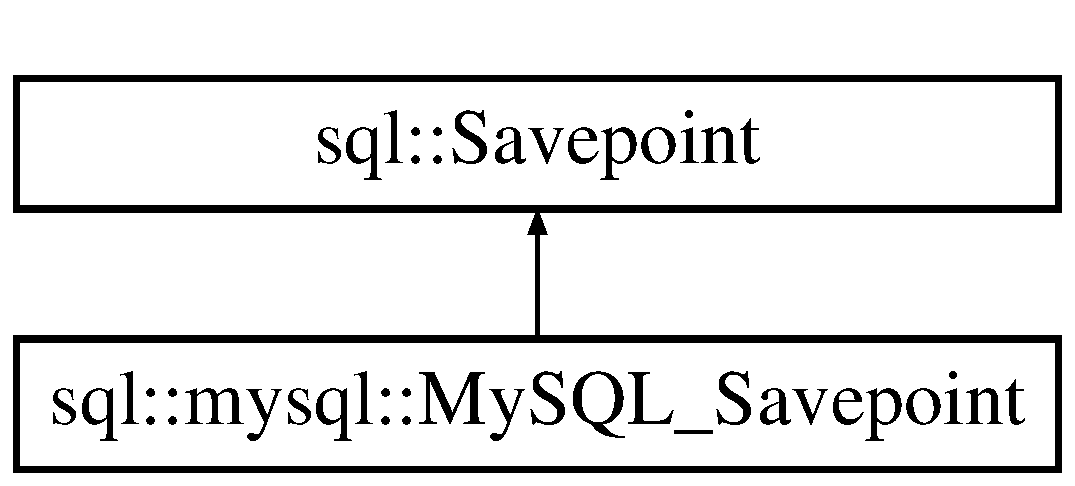
\includegraphics[height=2.000000cm]{classsql_1_1_savepoint}
\end{center}
\end{figure}
\subsection*{Public Member Functions}
\begin{DoxyCompactItemize}
\item 
\hypertarget{classsql_1_1_savepoint_a19c0a222303458f74ca16cb05ab50f4a}{}\label{classsql_1_1_savepoint_a19c0a222303458f74ca16cb05ab50f4a} 
virtual int {\bfseries get\+Savepoint\+Id} ()=0
\item 
\hypertarget{classsql_1_1_savepoint_ade620eb2f7c8caccaf5d8fa4f8242be9}{}\label{classsql_1_1_savepoint_ade620eb2f7c8caccaf5d8fa4f8242be9} 
virtual \hyperlink{classsql_1_1_s_q_l_string}{sql\+::\+S\+Q\+L\+String} {\bfseries get\+Savepoint\+Name} ()=0
\end{DoxyCompactItemize}
\subsection*{Private Member Functions}
\begin{DoxyCompactItemize}
\item 
\hypertarget{classsql_1_1_savepoint_abc59bfb9bdcc8e426dc7d7b13ed348da}{}\label{classsql_1_1_savepoint_abc59bfb9bdcc8e426dc7d7b13ed348da} 
{\bfseries Savepoint} (const \hyperlink{classsql_1_1_savepoint}{Savepoint} \&)
\item 
\hypertarget{classsql_1_1_savepoint_a5836938392c757c0430344424757198f}{}\label{classsql_1_1_savepoint_a5836938392c757c0430344424757198f} 
void {\bfseries operator=} (\hyperlink{classsql_1_1_savepoint}{Savepoint} \&)
\end{DoxyCompactItemize}


The documentation for this class was generated from the following file\+:\begin{DoxyCompactItemize}
\item 
E\+:/projekt\+\_\+cpp\+\_\+magazyn/projekt/\+Magazyn/\+Magazyn/\+Magazyn/mysql/include/cppconn/connection.\+h\end{DoxyCompactItemize}

\hypertarget{classsql_1_1_s_q_l_exception}{}\section{sql\+:\+:S\+Q\+L\+Exception Class Reference}
\label{classsql_1_1_s_q_l_exception}\index{sql\+::\+S\+Q\+L\+Exception@{sql\+::\+S\+Q\+L\+Exception}}
Inheritance diagram for sql\+:\+:S\+Q\+L\+Exception\+:\begin{figure}[H]
\begin{center}
\leavevmode
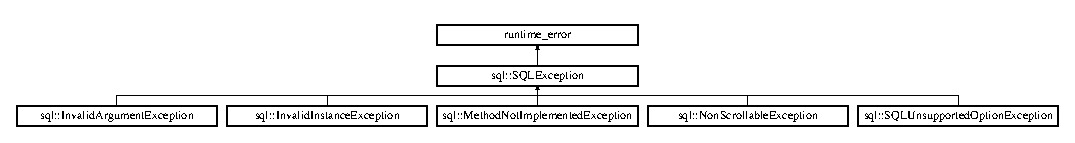
\includegraphics[height=1.467249cm]{classsql_1_1_s_q_l_exception}
\end{center}
\end{figure}
\subsection*{Public Member Functions}
\begin{DoxyCompactItemize}
\item 
\hypertarget{classsql_1_1_s_q_l_exception_afd6b5c61f3fd1608d88c77ce23553296}{}\label{classsql_1_1_s_q_l_exception_afd6b5c61f3fd1608d88c77ce23553296} 
{\bfseries S\+Q\+L\+Exception} (const \hyperlink{classsql_1_1_s_q_l_exception}{S\+Q\+L\+Exception} \&e)
\item 
\hypertarget{classsql_1_1_s_q_l_exception_aa35841915a5b1f5b71a6242e42015393}{}\label{classsql_1_1_s_q_l_exception_aa35841915a5b1f5b71a6242e42015393} 
{\bfseries S\+Q\+L\+Exception} (const std\+::string \&reason, const std\+::string \&S\+Q\+L\+State, int vendor\+Code)
\item 
\hypertarget{classsql_1_1_s_q_l_exception_a6d039899538ac3dbfa45a6863535e9c2}{}\label{classsql_1_1_s_q_l_exception_a6d039899538ac3dbfa45a6863535e9c2} 
{\bfseries S\+Q\+L\+Exception} (const std\+::string \&reason, const std\+::string \&S\+Q\+L\+State)
\item 
\hypertarget{classsql_1_1_s_q_l_exception_acdddee0d584c9f9e9cd50a926366fa94}{}\label{classsql_1_1_s_q_l_exception_acdddee0d584c9f9e9cd50a926366fa94} 
{\bfseries S\+Q\+L\+Exception} (const std\+::string \&reason)
\item 
\hypertarget{classsql_1_1_s_q_l_exception_a47de7e92cd45d5829bf44eefd24c4b93}{}\label{classsql_1_1_s_q_l_exception_a47de7e92cd45d5829bf44eefd24c4b93} 
const std\+::string \& {\bfseries get\+S\+Q\+L\+State} () const
\item 
\hypertarget{classsql_1_1_s_q_l_exception_a803dd506d802e196ad4af4f9839f00ed}{}\label{classsql_1_1_s_q_l_exception_a803dd506d802e196ad4af4f9839f00ed} 
const char $\ast$ {\bfseries get\+S\+Q\+L\+State\+C\+Str} () const
\item 
\hypertarget{classsql_1_1_s_q_l_exception_a3789c7cdd37233dae5fcb8cff387b4df}{}\label{classsql_1_1_s_q_l_exception_a3789c7cdd37233dae5fcb8cff387b4df} 
int {\bfseries get\+Error\+Code} () const
\end{DoxyCompactItemize}
\subsection*{Protected Attributes}
\begin{DoxyCompactItemize}
\item 
\hypertarget{classsql_1_1_s_q_l_exception_a0c8620ab60af316d2282fbdd112911f2}{}\label{classsql_1_1_s_q_l_exception_a0c8620ab60af316d2282fbdd112911f2} 
const std\+::string {\bfseries sql\+\_\+state}
\item 
\hypertarget{classsql_1_1_s_q_l_exception_ab9c454465e9929c87c090055e88b097b}{}\label{classsql_1_1_s_q_l_exception_ab9c454465e9929c87c090055e88b097b} 
const int {\bfseries err\+No}
\end{DoxyCompactItemize}


The documentation for this class was generated from the following file\+:\begin{DoxyCompactItemize}
\item 
E\+:/projekt\+\_\+cpp\+\_\+magazyn/projekt/\+Magazyn/\+Magazyn/\+Magazyn/mysql/include/cppconn/exception.\+h\end{DoxyCompactItemize}

\hypertarget{classsql_1_1_s_q_l_string}{}\section{sql\+:\+:S\+Q\+L\+String Class Reference}
\label{classsql_1_1_s_q_l_string}\index{sql\+::\+S\+Q\+L\+String@{sql\+::\+S\+Q\+L\+String}}
\subsection*{Public Member Functions}
\begin{DoxyCompactItemize}
\item 
\hypertarget{classsql_1_1_s_q_l_string_aa13d55ec3b3df1c841f755e24d4e28c9}{}\label{classsql_1_1_s_q_l_string_aa13d55ec3b3df1c841f755e24d4e28c9} 
{\bfseries S\+Q\+L\+String} (const \hyperlink{classsql_1_1_s_q_l_string}{S\+Q\+L\+String} \&other)
\item 
\hypertarget{classsql_1_1_s_q_l_string_a84644c05a801034d354b8bd10d2d8f72}{}\label{classsql_1_1_s_q_l_string_a84644c05a801034d354b8bd10d2d8f72} 
{\bfseries S\+Q\+L\+String} (const std\+::string \&other)
\item 
\hypertarget{classsql_1_1_s_q_l_string_a2566ad6c873e9c4c075503c2a850c7e5}{}\label{classsql_1_1_s_q_l_string_a2566ad6c873e9c4c075503c2a850c7e5} 
{\bfseries S\+Q\+L\+String} (const char other\mbox{[}$\,$\mbox{]})
\item 
\hypertarget{classsql_1_1_s_q_l_string_acd5dd85fcb890629c319ef55f445a2ac}{}\label{classsql_1_1_s_q_l_string_acd5dd85fcb890629c319ef55f445a2ac} 
{\bfseries S\+Q\+L\+String} (const char $\ast$s, size\+\_\+t n)
\item 
\hypertarget{classsql_1_1_s_q_l_string_adec7c9d6eec34ef339fc9da6e149b841}{}\label{classsql_1_1_s_q_l_string_adec7c9d6eec34ef339fc9da6e149b841} 
const \hyperlink{classsql_1_1_s_q_l_string}{S\+Q\+L\+String} \& {\bfseries operator=} (const char $\ast$s)
\item 
\hypertarget{classsql_1_1_s_q_l_string_a0a7c0cf3ba73ed9a174408be19ea1024}{}\label{classsql_1_1_s_q_l_string_a0a7c0cf3ba73ed9a174408be19ea1024} 
const \hyperlink{classsql_1_1_s_q_l_string}{S\+Q\+L\+String} \& {\bfseries operator=} (const std\+::string \&rhs)
\item 
\hypertarget{classsql_1_1_s_q_l_string_a40a973cbd4d20c436fbb027515e7acf0}{}\label{classsql_1_1_s_q_l_string_a40a973cbd4d20c436fbb027515e7acf0} 
const \hyperlink{classsql_1_1_s_q_l_string}{S\+Q\+L\+String} \& {\bfseries operator=} (const \hyperlink{classsql_1_1_s_q_l_string}{S\+Q\+L\+String} \&rhs)
\item 
\hypertarget{classsql_1_1_s_q_l_string_a4d1e10a51df4e9fc9856cfe7671129c1}{}\label{classsql_1_1_s_q_l_string_a4d1e10a51df4e9fc9856cfe7671129c1} 
{\bfseries operator const std\+::string \&} () const
\item 
std\+::string $\ast$ \hyperlink{classsql_1_1_s_q_l_string_a9a73b4b85edeea38025068914fc7c392}{operator-\/$>$} ()
\item 
\hypertarget{classsql_1_1_s_q_l_string_abb7aa8481365854f4766a31f80c4f84e}{}\label{classsql_1_1_s_q_l_string_abb7aa8481365854f4766a31f80c4f84e} 
int {\bfseries compare} (const \hyperlink{classsql_1_1_s_q_l_string}{S\+Q\+L\+String} \&str) const
\item 
\hypertarget{classsql_1_1_s_q_l_string_af65f75aaac05255a5e58219519ab5049}{}\label{classsql_1_1_s_q_l_string_af65f75aaac05255a5e58219519ab5049} 
int {\bfseries compare} (const char $\ast$s) const
\item 
\hypertarget{classsql_1_1_s_q_l_string_a11fe11219258d1f2390319ab41d156ee}{}\label{classsql_1_1_s_q_l_string_a11fe11219258d1f2390319ab41d156ee} 
int {\bfseries compare} (size\+\_\+t pos1, size\+\_\+t n1, const char $\ast$s) const
\item 
\hypertarget{classsql_1_1_s_q_l_string_a1a5f2c1258e23382a3206933364cfae9}{}\label{classsql_1_1_s_q_l_string_a1a5f2c1258e23382a3206933364cfae9} 
int {\bfseries case\+Compare} (const \hyperlink{classsql_1_1_s_q_l_string}{S\+Q\+L\+String} \&s) const
\item 
\hypertarget{classsql_1_1_s_q_l_string_a8b737f00858b2fd538e45de7f1c0fc58}{}\label{classsql_1_1_s_q_l_string_a8b737f00858b2fd538e45de7f1c0fc58} 
int {\bfseries case\+Compare} (const char $\ast$s) const
\item 
\hypertarget{classsql_1_1_s_q_l_string_ae7d0364b1c4bb90a622d369f080deac5}{}\label{classsql_1_1_s_q_l_string_ae7d0364b1c4bb90a622d369f080deac5} 
int {\bfseries case\+Compare} (size\+\_\+t pos1, size\+\_\+t n1, const char $\ast$s) const
\item 
\hypertarget{classsql_1_1_s_q_l_string_a923bf7c325d594d9e72b162f11fa9fd7}{}\label{classsql_1_1_s_q_l_string_a923bf7c325d594d9e72b162f11fa9fd7} 
const std\+::string \& {\bfseries as\+Std\+String} () const
\item 
\hypertarget{classsql_1_1_s_q_l_string_aaada0a7bb05515055b99e9f68c91bb78}{}\label{classsql_1_1_s_q_l_string_aaada0a7bb05515055b99e9f68c91bb78} 
const char $\ast$ {\bfseries c\+\_\+str} () const
\item 
\hypertarget{classsql_1_1_s_q_l_string_a36d8345110c4cc0aa61826116c196025}{}\label{classsql_1_1_s_q_l_string_a36d8345110c4cc0aa61826116c196025} 
size\+\_\+t {\bfseries length} () const
\item 
\hypertarget{classsql_1_1_s_q_l_string_a6877e186cc021a10a512e3446f67d7c5}{}\label{classsql_1_1_s_q_l_string_a6877e186cc021a10a512e3446f67d7c5} 
\hyperlink{classsql_1_1_s_q_l_string}{S\+Q\+L\+String} \& {\bfseries append} (const std\+::string \&str)
\item 
\hypertarget{classsql_1_1_s_q_l_string_a86b717dd5f5ca3b3117d50cd771cdf5d}{}\label{classsql_1_1_s_q_l_string_a86b717dd5f5ca3b3117d50cd771cdf5d} 
\hyperlink{classsql_1_1_s_q_l_string}{S\+Q\+L\+String} \& {\bfseries append} (const char $\ast$s)
\item 
\hypertarget{classsql_1_1_s_q_l_string_a20cfdb4b8d6b0750738606ab79619fb6}{}\label{classsql_1_1_s_q_l_string_a20cfdb4b8d6b0750738606ab79619fb6} 
const char \& {\bfseries operator\mbox{[}$\,$\mbox{]}} (size\+\_\+t pos) const
\item 
\hypertarget{classsql_1_1_s_q_l_string_a6a45c5e478b144a1d7e511d6d4040c07}{}\label{classsql_1_1_s_q_l_string_a6a45c5e478b144a1d7e511d6d4040c07} 
size\+\_\+t {\bfseries find} (char c, size\+\_\+t pos=0) const
\item 
\hypertarget{classsql_1_1_s_q_l_string_abb1323aa1f298d6550a8541f512b2a0f}{}\label{classsql_1_1_s_q_l_string_abb1323aa1f298d6550a8541f512b2a0f} 
size\+\_\+t {\bfseries find} (const \hyperlink{classsql_1_1_s_q_l_string}{S\+Q\+L\+String} \&s, size\+\_\+t pos=0) const
\item 
\hypertarget{classsql_1_1_s_q_l_string_a625fc710708a33603cb5705beea957bf}{}\label{classsql_1_1_s_q_l_string_a625fc710708a33603cb5705beea957bf} 
\hyperlink{classsql_1_1_s_q_l_string}{S\+Q\+L\+String} {\bfseries substr} (size\+\_\+t pos=0, size\+\_\+t n=npos) const
\item 
\hypertarget{classsql_1_1_s_q_l_string_aa96d107eb08a84bc6eace9a251e76bc1}{}\label{classsql_1_1_s_q_l_string_aa96d107eb08a84bc6eace9a251e76bc1} 
const \hyperlink{classsql_1_1_s_q_l_string}{S\+Q\+L\+String} \& {\bfseries replace} (size\+\_\+t pos1, size\+\_\+t n1, const \hyperlink{classsql_1_1_s_q_l_string}{S\+Q\+L\+String} \&s)
\item 
\hypertarget{classsql_1_1_s_q_l_string_ace6b7ff4e733bc4ee3f5572c9a19ee8a}{}\label{classsql_1_1_s_q_l_string_ace6b7ff4e733bc4ee3f5572c9a19ee8a} 
size\+\_\+t {\bfseries find\+\_\+first\+\_\+of} (char c, size\+\_\+t pos=0) const
\item 
\hypertarget{classsql_1_1_s_q_l_string_a9c90aefe9eec15b80b9a1dd40ce83a05}{}\label{classsql_1_1_s_q_l_string_a9c90aefe9eec15b80b9a1dd40ce83a05} 
size\+\_\+t {\bfseries find\+\_\+last\+\_\+of} (char c, size\+\_\+t pos=npos) const
\item 
\hypertarget{classsql_1_1_s_q_l_string_ad6e9824838e50e0b10bae83ead869d11}{}\label{classsql_1_1_s_q_l_string_ad6e9824838e50e0b10bae83ead869d11} 
const \hyperlink{classsql_1_1_s_q_l_string}{S\+Q\+L\+String} \& {\bfseries operator+=} (const \hyperlink{classsql_1_1_s_q_l_string}{S\+Q\+L\+String} \&op2)
\end{DoxyCompactItemize}
\subsection*{Static Public Attributes}
\begin{DoxyCompactItemize}
\item 
\hypertarget{classsql_1_1_s_q_l_string_ab877913be4071b769350929953825c35}{}\label{classsql_1_1_s_q_l_string_ab877913be4071b769350929953825c35} 
static const size\+\_\+t {\bfseries npos} = std\+::string\+::npos
\end{DoxyCompactItemize}
\subsection*{Private Attributes}
\begin{DoxyCompactItemize}
\item 
\hypertarget{classsql_1_1_s_q_l_string_a8210f5235dd913e114d877c0a1ce30aa}{}\label{classsql_1_1_s_q_l_string_a8210f5235dd913e114d877c0a1ce30aa} 
std\+::string {\bfseries real\+Str}
\end{DoxyCompactItemize}


\subsection{Member Function Documentation}
\hypertarget{classsql_1_1_s_q_l_string_a9a73b4b85edeea38025068914fc7c392}{}\label{classsql_1_1_s_q_l_string_a9a73b4b85edeea38025068914fc7c392} 
\index{sql\+::\+S\+Q\+L\+String@{sql\+::\+S\+Q\+L\+String}!operator-\/$>$@{operator-\/$>$}}
\index{operator-\/$>$@{operator-\/$>$}!sql\+::\+S\+Q\+L\+String@{sql\+::\+S\+Q\+L\+String}}
\subsubsection{\texorpdfstring{operator-\/$>$()}{operator->()}}
{\footnotesize\ttfamily std\+::string$\ast$ sql\+::\+S\+Q\+L\+String\+::operator-\/$>$ (\begin{DoxyParamCaption}{ }\end{DoxyParamCaption})\hspace{0.3cm}{\ttfamily [inline]}}

For access std\+::string methods. Not sure we need it. Makes it look like some smart ptr. possibly operator$\ast$ -\/ will look even more like smart ptr 

The documentation for this class was generated from the following file\+:\begin{DoxyCompactItemize}
\item 
E\+:/projekt\+\_\+cpp\+\_\+magazyn/projekt/\+Magazyn/\+Magazyn/\+Magazyn/mysql/include/cppconn/sqlstring.\+h\end{DoxyCompactItemize}

\hypertarget{structsql_1_1_s_q_l_unsupported_option_exception}{}\section{sql\+:\+:S\+Q\+L\+Unsupported\+Option\+Exception Struct Reference}
\label{structsql_1_1_s_q_l_unsupported_option_exception}\index{sql\+::\+S\+Q\+L\+Unsupported\+Option\+Exception@{sql\+::\+S\+Q\+L\+Unsupported\+Option\+Exception}}
Inheritance diagram for sql\+:\+:S\+Q\+L\+Unsupported\+Option\+Exception\+:\begin{figure}[H]
\begin{center}
\leavevmode
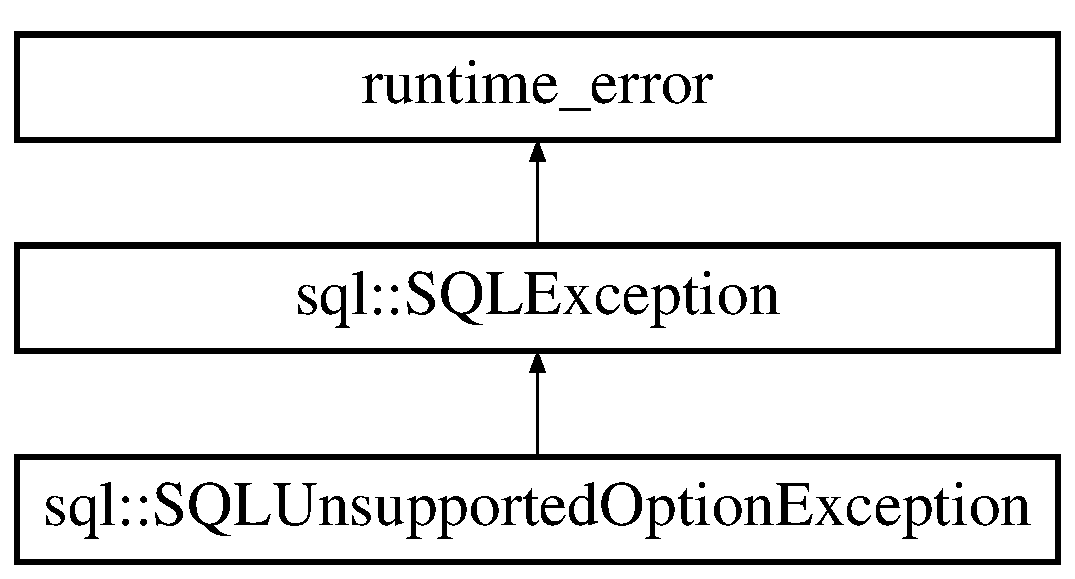
\includegraphics[height=3.000000cm]{structsql_1_1_s_q_l_unsupported_option_exception}
\end{center}
\end{figure}
\subsection*{Public Member Functions}
\begin{DoxyCompactItemize}
\item 
\hypertarget{structsql_1_1_s_q_l_unsupported_option_exception_ac2cb843126b8d145a1563b840f08e7b6}{}\label{structsql_1_1_s_q_l_unsupported_option_exception_ac2cb843126b8d145a1563b840f08e7b6} 
{\bfseries S\+Q\+L\+Unsupported\+Option\+Exception} (const \hyperlink{structsql_1_1_s_q_l_unsupported_option_exception}{S\+Q\+L\+Unsupported\+Option\+Exception} \&e, const std\+::string conn\+\_\+option)
\item 
\hypertarget{structsql_1_1_s_q_l_unsupported_option_exception_a29dad1765e43c979263d66089a381f90}{}\label{structsql_1_1_s_q_l_unsupported_option_exception_a29dad1765e43c979263d66089a381f90} 
{\bfseries S\+Q\+L\+Unsupported\+Option\+Exception} (const std\+::string \&reason, const std\+::string conn\+\_\+option)
\item 
\hypertarget{structsql_1_1_s_q_l_unsupported_option_exception_af7a71c50ba83c6ab575a968947088af8}{}\label{structsql_1_1_s_q_l_unsupported_option_exception_af7a71c50ba83c6ab575a968947088af8} 
const char $\ast$ {\bfseries get\+Connection\+Option} () const
\end{DoxyCompactItemize}
\subsection*{Protected Attributes}
\begin{DoxyCompactItemize}
\item 
\hypertarget{structsql_1_1_s_q_l_unsupported_option_exception_a8a1789a364522449f67839c018a0bcc6}{}\label{structsql_1_1_s_q_l_unsupported_option_exception_a8a1789a364522449f67839c018a0bcc6} 
const std\+::string {\bfseries option}
\end{DoxyCompactItemize}


The documentation for this struct was generated from the following file\+:\begin{DoxyCompactItemize}
\item 
E\+:/projekt\+\_\+cpp\+\_\+magazyn/projekt/\+Magazyn/\+Magazyn/\+Magazyn/mysql/include/cppconn/exception.\+h\end{DoxyCompactItemize}

\hypertarget{classsql_1_1_s_q_l_warning}{}\section{sql\+:\+:S\+Q\+L\+Warning Class Reference}
\label{classsql_1_1_s_q_l_warning}\index{sql\+::\+S\+Q\+L\+Warning@{sql\+::\+S\+Q\+L\+Warning}}
\subsection*{Public Member Functions}
\begin{DoxyCompactItemize}
\item 
\hypertarget{classsql_1_1_s_q_l_warning_a660df3d9cd98a5ac7bc8bc9edf7cc8b1}{}\label{classsql_1_1_s_q_l_warning_a660df3d9cd98a5ac7bc8bc9edf7cc8b1} 
virtual const \hyperlink{classsql_1_1_s_q_l_string}{sql\+::\+S\+Q\+L\+String} \& {\bfseries get\+Message} () const =0
\item 
\hypertarget{classsql_1_1_s_q_l_warning_a47e6991427a672be4cbc0e32295aea28}{}\label{classsql_1_1_s_q_l_warning_a47e6991427a672be4cbc0e32295aea28} 
virtual const \hyperlink{classsql_1_1_s_q_l_string}{sql\+::\+S\+Q\+L\+String} \& {\bfseries get\+S\+Q\+L\+State} () const =0
\item 
\hypertarget{classsql_1_1_s_q_l_warning_a6c840336844c022bc1fd8ab8158da4ea}{}\label{classsql_1_1_s_q_l_warning_a6c840336844c022bc1fd8ab8158da4ea} 
virtual int {\bfseries get\+Error\+Code} () const =0
\item 
\hypertarget{classsql_1_1_s_q_l_warning_a37d3ffe0295388c82ca9cb8ed1d7e0d4}{}\label{classsql_1_1_s_q_l_warning_a37d3ffe0295388c82ca9cb8ed1d7e0d4} 
virtual const \hyperlink{classsql_1_1_s_q_l_warning}{S\+Q\+L\+Warning} $\ast$ {\bfseries get\+Next\+Warning} () const =0
\item 
\hypertarget{classsql_1_1_s_q_l_warning_acf0c7092bf4ef8cd4885471f20de76e0}{}\label{classsql_1_1_s_q_l_warning_acf0c7092bf4ef8cd4885471f20de76e0} 
virtual void {\bfseries set\+Next\+Warning} (const \hyperlink{classsql_1_1_s_q_l_warning}{S\+Q\+L\+Warning} $\ast$\+\_\+next)=0
\end{DoxyCompactItemize}
\subsection*{Protected Member Functions}
\begin{DoxyCompactItemize}
\item 
\hypertarget{classsql_1_1_s_q_l_warning_aead494b8feb63db50bb94cf7fac4f208}{}\label{classsql_1_1_s_q_l_warning_aead494b8feb63db50bb94cf7fac4f208} 
{\bfseries S\+Q\+L\+Warning} (const \hyperlink{classsql_1_1_s_q_l_warning}{S\+Q\+L\+Warning} \&e)
\end{DoxyCompactItemize}
\subsection*{Private Member Functions}
\begin{DoxyCompactItemize}
\item 
\hypertarget{classsql_1_1_s_q_l_warning_a383987b2b1d620afd5e61cc80c34ee63}{}\label{classsql_1_1_s_q_l_warning_a383987b2b1d620afd5e61cc80c34ee63} 
const \hyperlink{classsql_1_1_s_q_l_warning}{S\+Q\+L\+Warning} \& {\bfseries operator=} (const \hyperlink{classsql_1_1_s_q_l_warning}{S\+Q\+L\+Warning} \&rhs)
\end{DoxyCompactItemize}


The documentation for this class was generated from the following file\+:\begin{DoxyCompactItemize}
\item 
E\+:/projekt\+\_\+cpp\+\_\+magazyn/projekt/\+Magazyn/\+Magazyn/\+Magazyn/mysql/include/cppconn/warning.\+h\end{DoxyCompactItemize}

\hypertarget{classsql_1_1_statement}{}\section{sql\+:\+:Statement Class Reference}
\label{classsql_1_1_statement}\index{sql\+::\+Statement@{sql\+::\+Statement}}
Inheritance diagram for sql\+:\+:Statement\+:\begin{figure}[H]
\begin{center}
\leavevmode
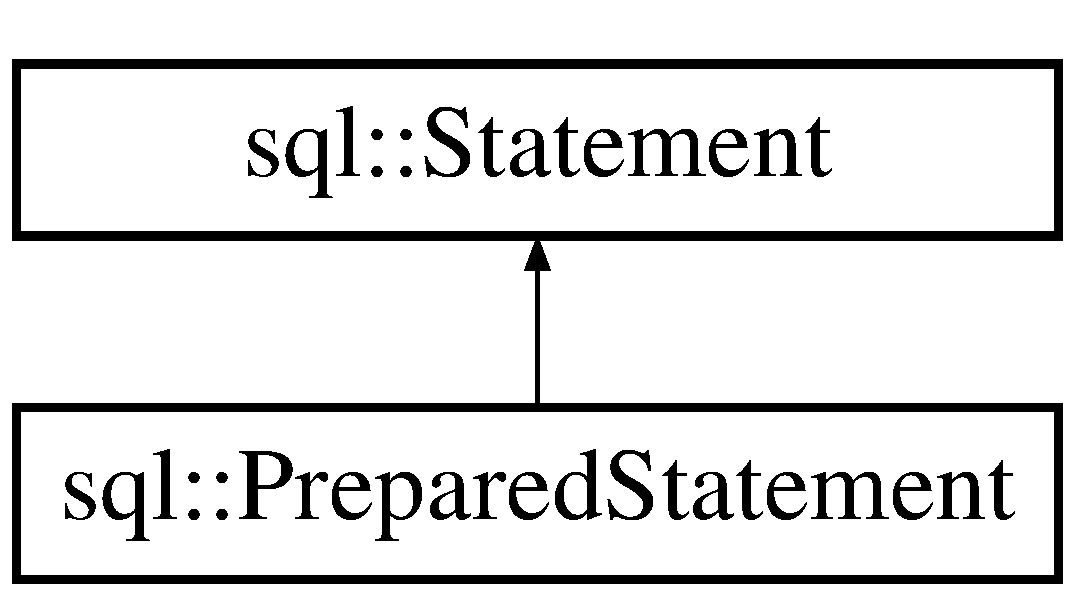
\includegraphics[height=2.000000cm]{classsql_1_1_statement}
\end{center}
\end{figure}
\subsection*{Public Member Functions}
\begin{DoxyCompactItemize}
\item 
\hypertarget{classsql_1_1_statement_a2c3085011600e4208f94ec8d2f7707c3}{}\label{classsql_1_1_statement_a2c3085011600e4208f94ec8d2f7707c3} 
virtual \hyperlink{classsql_1_1_connection}{Connection} $\ast$ {\bfseries get\+Connection} ()=0
\item 
\hypertarget{classsql_1_1_statement_afb9b8908e2d2a7f30c760e307feeb857}{}\label{classsql_1_1_statement_afb9b8908e2d2a7f30c760e307feeb857} 
virtual void {\bfseries cancel} ()=0
\item 
\hypertarget{classsql_1_1_statement_a254f97d835d62d9a2e7400409e48ea34}{}\label{classsql_1_1_statement_a254f97d835d62d9a2e7400409e48ea34} 
virtual void {\bfseries clear\+Warnings} ()=0
\item 
\hypertarget{classsql_1_1_statement_ae781a85fe88efb3cf35cd5e0310bb4ed}{}\label{classsql_1_1_statement_ae781a85fe88efb3cf35cd5e0310bb4ed} 
virtual void {\bfseries close} ()=0
\item 
\hypertarget{classsql_1_1_statement_aa5a54d7d71c8d622d8acf578cbbe6f16}{}\label{classsql_1_1_statement_aa5a54d7d71c8d622d8acf578cbbe6f16} 
virtual bool {\bfseries execute} (const \hyperlink{classsql_1_1_s_q_l_string}{sql\+::\+S\+Q\+L\+String} \&sql)=0
\item 
\hypertarget{classsql_1_1_statement_ae3afe5ea2a8bf0cc7d5eac917da7bd19}{}\label{classsql_1_1_statement_ae3afe5ea2a8bf0cc7d5eac917da7bd19} 
virtual \hyperlink{classsql_1_1_result_set}{Result\+Set} $\ast$ {\bfseries execute\+Query} (const \hyperlink{classsql_1_1_s_q_l_string}{sql\+::\+S\+Q\+L\+String} \&sql)=0
\item 
\hypertarget{classsql_1_1_statement_a178c0510e1ea9e906e1bfd6638c7f6ca}{}\label{classsql_1_1_statement_a178c0510e1ea9e906e1bfd6638c7f6ca} 
virtual int {\bfseries execute\+Update} (const \hyperlink{classsql_1_1_s_q_l_string}{sql\+::\+S\+Q\+L\+String} \&sql)=0
\item 
\hypertarget{classsql_1_1_statement_a20a95dacaaf567d49e70af4522a7b64b}{}\label{classsql_1_1_statement_a20a95dacaaf567d49e70af4522a7b64b} 
virtual size\+\_\+t {\bfseries get\+Fetch\+Size} ()=0
\item 
\hypertarget{classsql_1_1_statement_a0f823e05b313b634b0cd0861f3b1d416}{}\label{classsql_1_1_statement_a0f823e05b313b634b0cd0861f3b1d416} 
virtual unsigned int {\bfseries get\+Max\+Field\+Size} ()=0
\item 
\hypertarget{classsql_1_1_statement_a2ca642c012e84b14191eecc3191466b3}{}\label{classsql_1_1_statement_a2ca642c012e84b14191eecc3191466b3} 
virtual uint64\+\_\+t {\bfseries get\+Max\+Rows} ()=0
\item 
\hypertarget{classsql_1_1_statement_a1cc03f400cb79ac740bb99f25a31d4d8}{}\label{classsql_1_1_statement_a1cc03f400cb79ac740bb99f25a31d4d8} 
virtual bool {\bfseries get\+More\+Results} ()=0
\item 
\hypertarget{classsql_1_1_statement_a4137a49581baaf8524131f686fd52f4f}{}\label{classsql_1_1_statement_a4137a49581baaf8524131f686fd52f4f} 
virtual unsigned int {\bfseries get\+Query\+Timeout} ()=0
\item 
\hypertarget{classsql_1_1_statement_ae1ea6eb2fd4de2a7716711f94aded8e0}{}\label{classsql_1_1_statement_ae1ea6eb2fd4de2a7716711f94aded8e0} 
virtual \hyperlink{classsql_1_1_result_set}{Result\+Set} $\ast$ {\bfseries get\+Result\+Set} ()=0
\item 
\hypertarget{classsql_1_1_statement_a8a00e6dc42f8c9c1171cf7f8a275b62b}{}\label{classsql_1_1_statement_a8a00e6dc42f8c9c1171cf7f8a275b62b} 
virtual sql\+::\+Result\+Set\+::enum\+\_\+type {\bfseries get\+Result\+Set\+Type} ()=0
\item 
\hypertarget{classsql_1_1_statement_a67326fb97e261aa919c73ce35fdf8784}{}\label{classsql_1_1_statement_a67326fb97e261aa919c73ce35fdf8784} 
virtual uint64\+\_\+t {\bfseries get\+Update\+Count} ()=0
\item 
\hypertarget{classsql_1_1_statement_ac05bc0fb234b66d58d9446837dd25c14}{}\label{classsql_1_1_statement_ac05bc0fb234b66d58d9446837dd25c14} 
virtual const \hyperlink{classsql_1_1_s_q_l_warning}{S\+Q\+L\+Warning} $\ast$ {\bfseries get\+Warnings} ()=0
\item 
\hypertarget{classsql_1_1_statement_a47125e21ac06a5fd48d45787dffa3459}{}\label{classsql_1_1_statement_a47125e21ac06a5fd48d45787dffa3459} 
virtual void {\bfseries set\+Cursor\+Name} (const \hyperlink{classsql_1_1_s_q_l_string}{sql\+::\+S\+Q\+L\+String} \&name)=0
\item 
\hypertarget{classsql_1_1_statement_a575bc70969296498ba409d2dcd8cc062}{}\label{classsql_1_1_statement_a575bc70969296498ba409d2dcd8cc062} 
virtual void {\bfseries set\+Escape\+Processing} (bool enable)=0
\item 
\hypertarget{classsql_1_1_statement_a8c8deb69ffd64a711d2b2b6d65747052}{}\label{classsql_1_1_statement_a8c8deb69ffd64a711d2b2b6d65747052} 
virtual void {\bfseries set\+Fetch\+Size} (size\+\_\+t rows)=0
\item 
\hypertarget{classsql_1_1_statement_a4cbc05f0c9dbc97237c6245fa5bfc46c}{}\label{classsql_1_1_statement_a4cbc05f0c9dbc97237c6245fa5bfc46c} 
virtual void {\bfseries set\+Max\+Field\+Size} (unsigned int max)=0
\item 
\hypertarget{classsql_1_1_statement_ad52108d248bd1272e8f80b53a549e51d}{}\label{classsql_1_1_statement_ad52108d248bd1272e8f80b53a549e51d} 
virtual void {\bfseries set\+Max\+Rows} (unsigned int max)=0
\item 
\hypertarget{classsql_1_1_statement_af3367d2f09798ad17d2e0605bc768a4f}{}\label{classsql_1_1_statement_af3367d2f09798ad17d2e0605bc768a4f} 
virtual void {\bfseries set\+Query\+Timeout} (unsigned int seconds)=0
\item 
\hypertarget{classsql_1_1_statement_a6d25bd789114a649f22af3aa940ef735}{}\label{classsql_1_1_statement_a6d25bd789114a649f22af3aa940ef735} 
virtual \hyperlink{classsql_1_1_statement}{Statement} $\ast$ {\bfseries set\+Result\+Set\+Type} (sql\+::\+Result\+Set\+::enum\+\_\+type type)=0
\end{DoxyCompactItemize}


The documentation for this class was generated from the following file\+:\begin{DoxyCompactItemize}
\item 
E\+:/projekt\+\_\+cpp\+\_\+magazyn/projekt/\+Magazyn/\+Magazyn/\+Magazyn/mysql/include/cppconn/statement.\+h\end{DoxyCompactItemize}

\hypertarget{classsql_1_1_variant}{}\section{sql\+:\+:Variant Class Reference}
\label{classsql_1_1_variant}\index{sql\+::\+Variant@{sql\+::\+Variant}}
\subsection*{Public Member Functions}
\begin{DoxyCompactItemize}
\item 
\hypertarget{classsql_1_1_variant_a3e45b2e2740ec0c4802494637e9206df}{}\label{classsql_1_1_variant_a3e45b2e2740ec0c4802494637e9206df} 
{\bfseries Variant} (const int \&i=0)
\item 
\hypertarget{classsql_1_1_variant_abc766ebf62d2430abf644089b4cd0176}{}\label{classsql_1_1_variant_abc766ebf62d2430abf644089b4cd0176} 
{\bfseries Variant} (const double \&i)
\item 
\hypertarget{classsql_1_1_variant_a6fb56c509635c8e1eb0ff78e538f0932}{}\label{classsql_1_1_variant_a6fb56c509635c8e1eb0ff78e538f0932} 
{\bfseries Variant} (const bool \&i)
\item 
\hypertarget{classsql_1_1_variant_a2c76e4cd5c0935728bd84d2c7c9dc34f}{}\label{classsql_1_1_variant_a2c76e4cd5c0935728bd84d2c7c9dc34f} 
{\bfseries Variant} (const std\+::string \&i)
\item 
\hypertarget{classsql_1_1_variant_af966a0c9980fcda78d14a3f2956aeea9}{}\label{classsql_1_1_variant_af966a0c9980fcda78d14a3f2956aeea9} 
{\bfseries Variant} (const \hyperlink{classsql_1_1_s_q_l_string}{sql\+::\+S\+Q\+L\+String} \&i)
\item 
\hypertarget{classsql_1_1_variant_aaa42466407cff394eaf165499c96a5ce}{}\label{classsql_1_1_variant_aaa42466407cff394eaf165499c96a5ce} 
{\bfseries Variant} (const std\+::list$<$ std\+::string $>$ \&i)
\item 
\hypertarget{classsql_1_1_variant_aff3232f730a6e14fb3425e8ff6631d92}{}\label{classsql_1_1_variant_aff3232f730a6e14fb3425e8ff6631d92} 
{\bfseries Variant} (const std\+::list$<$ \hyperlink{classsql_1_1_s_q_l_string}{sql\+::\+S\+Q\+L\+String} $>$ \&i)
\item 
\hypertarget{classsql_1_1_variant_acbfd8c447e90d791d8e7a26ac4147111}{}\label{classsql_1_1_variant_acbfd8c447e90d791d8e7a26ac4147111} 
{\bfseries Variant} (const std\+::map$<$ std\+::string, std\+::string $>$ \&i)
\item 
\hypertarget{classsql_1_1_variant_a2040d2456140a42a6f296286502d3a3d}{}\label{classsql_1_1_variant_a2040d2456140a42a6f296286502d3a3d} 
{\bfseries Variant} (const std\+::map$<$ \hyperlink{classsql_1_1_s_q_l_string}{sql\+::\+S\+Q\+L\+String}, \hyperlink{classsql_1_1_s_q_l_string}{sql\+::\+S\+Q\+L\+String} $>$ \&i)
\item 
\hypertarget{classsql_1_1_variant_ad3c0e0299b1a39feb507cf435143262a}{}\label{classsql_1_1_variant_ad3c0e0299b1a39feb507cf435143262a} 
{\bfseries Variant} (const \hyperlink{classsql_1_1_variant}{Variant} \&that)
\item 
\hypertarget{classsql_1_1_variant_a3776937e0bb01168bba0fd1ddec56718}{}\label{classsql_1_1_variant_a3776937e0bb01168bba0fd1ddec56718} 
\hyperlink{classsql_1_1_variant}{Variant} \& {\bfseries operator=} (const \hyperlink{classsql_1_1_variant}{Variant} \&that)
\item 
\hypertarget{classsql_1_1_variant_ab5e2e01b0fe270c02f97183de2fc8ffb}{}\label{classsql_1_1_variant_ab5e2e01b0fe270c02f97183de2fc8ffb} 
{\footnotesize template$<$class T $>$ }\\T $\ast$ {\bfseries get} () const
\end{DoxyCompactItemize}
\subsection*{Private Attributes}
\begin{DoxyCompactItemize}
\item 
\hypertarget{classsql_1_1_variant_a6c25156805d59d4725f03635a8b18160}{}\label{classsql_1_1_variant_a6c25156805d59d4725f03635a8b18160} 
\hyperlink{classsql_1_1_base_variant_impl}{Base\+Variant\+Impl} $\ast$ {\bfseries variant}
\end{DoxyCompactItemize}


The documentation for this class was generated from the following file\+:\begin{DoxyCompactItemize}
\item 
E\+:/projekt\+\_\+cpp\+\_\+magazyn/projekt/\+Magazyn/\+Magazyn/\+Magazyn/mysql/include/cppconn/variant.\+h\end{DoxyCompactItemize}

\hypertarget{classsql_1_1_variant_impl}{}\section{sql\+:\+:Variant\+Impl$<$ T $>$ Class Template Reference}
\label{classsql_1_1_variant_impl}\index{sql\+::\+Variant\+Impl$<$ T $>$@{sql\+::\+Variant\+Impl$<$ T $>$}}
Inheritance diagram for sql\+:\+:Variant\+Impl$<$ T $>$\+:\begin{figure}[H]
\begin{center}
\leavevmode
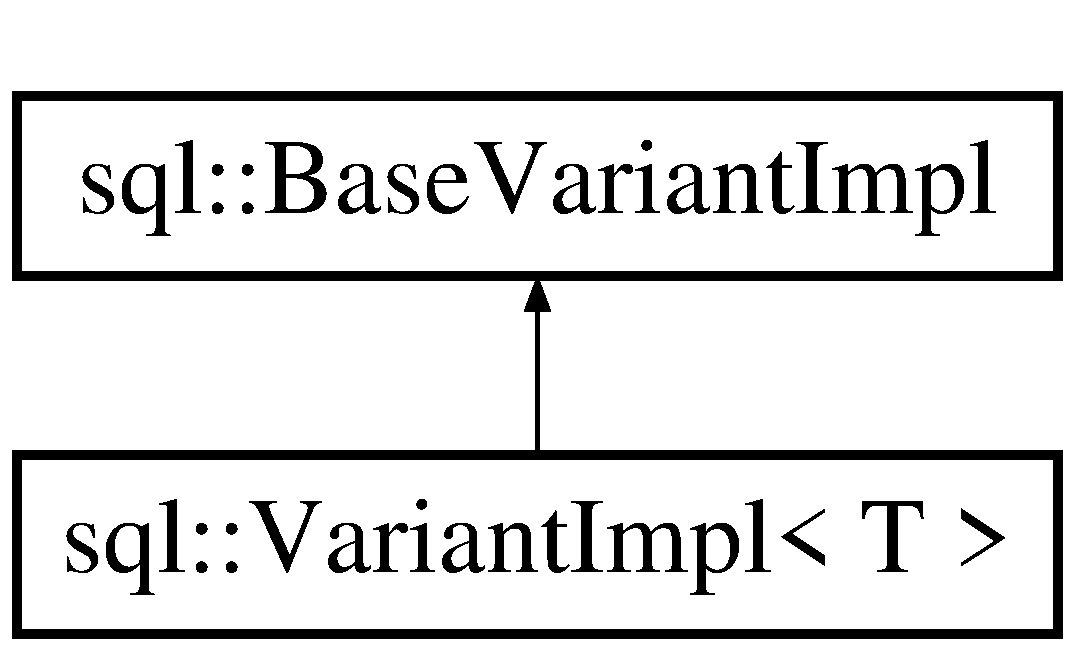
\includegraphics[height=2.000000cm]{classsql_1_1_variant_impl}
\end{center}
\end{figure}
\subsection*{Public Member Functions}
\begin{DoxyCompactItemize}
\item 
\hypertarget{classsql_1_1_variant_impl_a1136a66ff16556a8de22c6f571d9cb36}{}\label{classsql_1_1_variant_impl_a1136a66ff16556a8de22c6f571d9cb36} 
{\bfseries Variant\+Impl} (T i)
\item 
\hypertarget{classsql_1_1_variant_impl_aef2f99e7bd996f7d2f4b2344306b9cfb}{}\label{classsql_1_1_variant_impl_aef2f99e7bd996f7d2f4b2344306b9cfb} 
{\bfseries Variant\+Impl} (\hyperlink{classsql_1_1_variant_impl}{Variant\+Impl} \&that)
\item 
\hypertarget{classsql_1_1_variant_impl_a9fea2f2251f67498a82c6a42caf58f81}{}\label{classsql_1_1_variant_impl_a9fea2f2251f67498a82c6a42caf58f81} 
\hyperlink{classsql_1_1_variant_impl}{Variant\+Impl} \& {\bfseries operator=} (\hyperlink{classsql_1_1_variant_impl}{Variant\+Impl} \&that)
\item 
\hypertarget{classsql_1_1_variant_impl_a529173b4d305ad80d9a8f65c2497ee52}{}\label{classsql_1_1_variant_impl_a529173b4d305ad80d9a8f65c2497ee52} 
virtual \hyperlink{classsql_1_1_variant_impl}{Variant\+Impl} $\ast$ {\bfseries Clone} ()
\end{DoxyCompactItemize}
\subsection*{Private Member Functions}
\begin{DoxyCompactItemize}
\item 
\hypertarget{classsql_1_1_variant_impl_a11e5e5148a11c3013b41f5d8d144e67b}{}\label{classsql_1_1_variant_impl_a11e5e5148a11c3013b41f5d8d144e67b} 
void {\bfseries destroy\+\_\+content} ()
\item 
\hypertarget{classsql_1_1_variant_impl_a38b50b688f3b7e045e218bce007042fb}{}\label{classsql_1_1_variant_impl_a38b50b688f3b7e045e218bce007042fb} 
void {\bfseries copy\+\_\+content} (\hyperlink{classsql_1_1_base_variant_impl}{Base\+Variant\+Impl} \&that)
\end{DoxyCompactItemize}
\subsection*{Additional Inherited Members}


The documentation for this class was generated from the following file\+:\begin{DoxyCompactItemize}
\item 
E\+:/projekt\+\_\+cpp\+\_\+magazyn/projekt/\+Magazyn/\+Magazyn/\+Magazyn/mysql/include/cppconn/variant.\+h\end{DoxyCompactItemize}

\hypertarget{classsql_1_1_variant_list}{}\section{sql\+:\+:Variant\+List$<$ T $>$ Class Template Reference}
\label{classsql_1_1_variant_list}\index{sql\+::\+Variant\+List$<$ T $>$@{sql\+::\+Variant\+List$<$ T $>$}}
Inheritance diagram for sql\+:\+:Variant\+List$<$ T $>$\+:\begin{figure}[H]
\begin{center}
\leavevmode
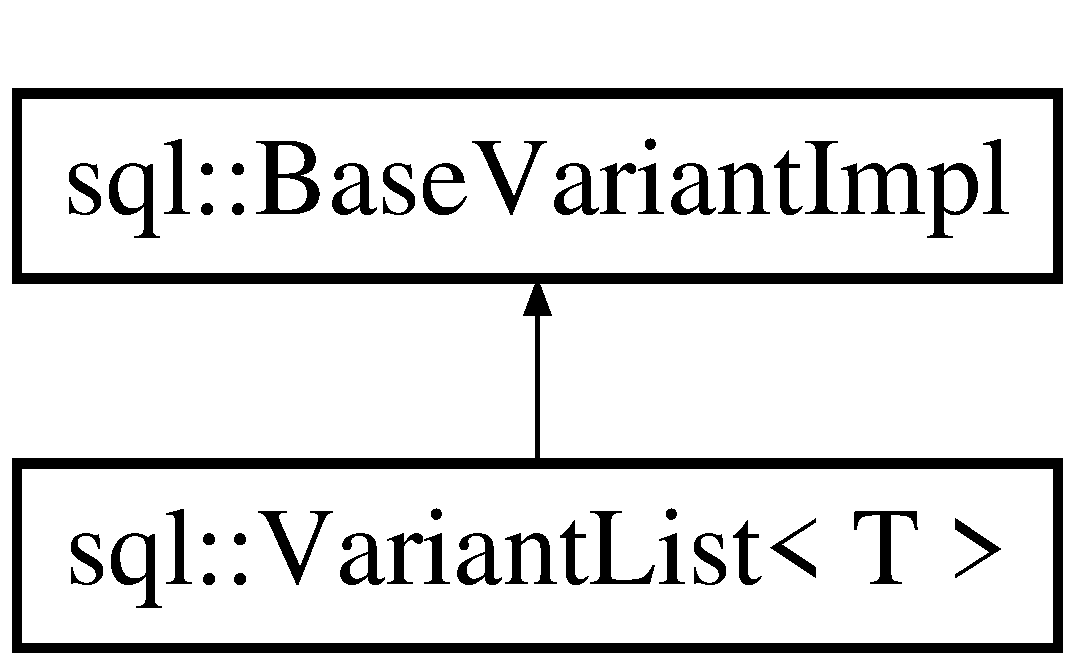
\includegraphics[height=2.000000cm]{classsql_1_1_variant_list}
\end{center}
\end{figure}
\subsection*{Public Member Functions}
\begin{DoxyCompactItemize}
\item 
\hypertarget{classsql_1_1_variant_list_a5973123c3f878ad52f5fa55f9a5bcbf9}{}\label{classsql_1_1_variant_list_a5973123c3f878ad52f5fa55f9a5bcbf9} 
{\bfseries Variant\+List} (T i)
\item 
\hypertarget{classsql_1_1_variant_list_a9317f749d181ed90bee721fb68491e27}{}\label{classsql_1_1_variant_list_a9317f749d181ed90bee721fb68491e27} 
{\bfseries Variant\+List} (\hyperlink{classsql_1_1_variant_list}{Variant\+List} \&that)
\item 
\hypertarget{classsql_1_1_variant_list_aa8ce979522fc282003edc70e97e5c080}{}\label{classsql_1_1_variant_list_aa8ce979522fc282003edc70e97e5c080} 
\hyperlink{classsql_1_1_variant_list}{Variant\+List} \& {\bfseries operator=} (\hyperlink{classsql_1_1_variant_list}{Variant\+List} \&that)
\item 
\hypertarget{classsql_1_1_variant_list_adc6519883b262a78ecddc51925f7ce4b}{}\label{classsql_1_1_variant_list_adc6519883b262a78ecddc51925f7ce4b} 
virtual \hyperlink{classsql_1_1_variant_list}{Variant\+List} $\ast$ {\bfseries Clone} ()
\end{DoxyCompactItemize}
\subsection*{Private Member Functions}
\begin{DoxyCompactItemize}
\item 
\hypertarget{classsql_1_1_variant_list_a86186fc1d8a877b98d7f39cfbe813380}{}\label{classsql_1_1_variant_list_a86186fc1d8a877b98d7f39cfbe813380} 
void {\bfseries destroy\+\_\+content} ()
\item 
\hypertarget{classsql_1_1_variant_list_a2bca42e5938c59c6a17cb5dbeb246f90}{}\label{classsql_1_1_variant_list_a2bca42e5938c59c6a17cb5dbeb246f90} 
void {\bfseries copy\+\_\+content} (\hyperlink{classsql_1_1_variant_list}{Variant\+List} \&var)
\end{DoxyCompactItemize}
\subsection*{Additional Inherited Members}


The documentation for this class was generated from the following file\+:\begin{DoxyCompactItemize}
\item 
E\+:/projekt\+\_\+cpp\+\_\+magazyn/projekt/\+Magazyn/\+Magazyn/\+Magazyn/mysql/include/cppconn/variant.\+h\end{DoxyCompactItemize}

\hypertarget{classsql_1_1_variant_map}{}\section{sql\+:\+:Variant\+Map$<$ T $>$ Class Template Reference}
\label{classsql_1_1_variant_map}\index{sql\+::\+Variant\+Map$<$ T $>$@{sql\+::\+Variant\+Map$<$ T $>$}}
Inheritance diagram for sql\+:\+:Variant\+Map$<$ T $>$\+:\begin{figure}[H]
\begin{center}
\leavevmode
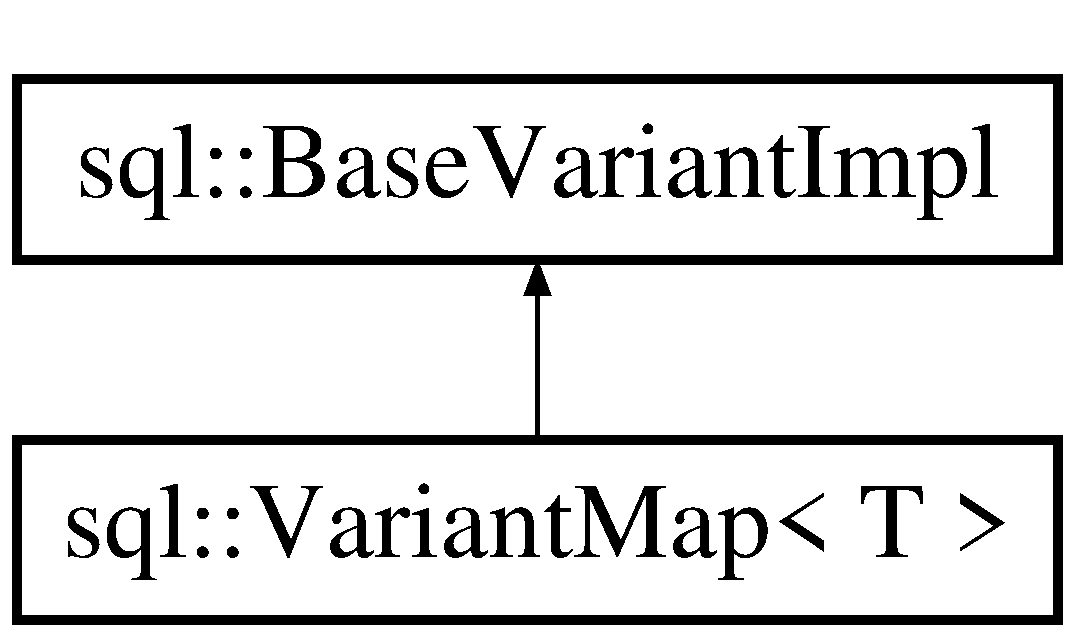
\includegraphics[height=2.000000cm]{classsql_1_1_variant_map}
\end{center}
\end{figure}
\subsection*{Public Member Functions}
\begin{DoxyCompactItemize}
\item 
\hypertarget{classsql_1_1_variant_map_a57a3ef9f7780d378e7e8ec2d6f2782db}{}\label{classsql_1_1_variant_map_a57a3ef9f7780d378e7e8ec2d6f2782db} 
{\bfseries Variant\+Map} (T i)
\item 
\hypertarget{classsql_1_1_variant_map_a460d04a63f6efdb9f8e23f541faefb39}{}\label{classsql_1_1_variant_map_a460d04a63f6efdb9f8e23f541faefb39} 
{\bfseries Variant\+Map} (\hyperlink{classsql_1_1_variant_map}{Variant\+Map} \&that)
\item 
\hypertarget{classsql_1_1_variant_map_ac1962c1da18635bc551264e1821dc5d2}{}\label{classsql_1_1_variant_map_ac1962c1da18635bc551264e1821dc5d2} 
\hyperlink{classsql_1_1_variant_map}{Variant\+Map} \& {\bfseries operator=} (\hyperlink{classsql_1_1_variant_map}{Variant\+Map} \&that)
\item 
\hypertarget{classsql_1_1_variant_map_a6fad5d2f5006961456fb8f8ef649c0bc}{}\label{classsql_1_1_variant_map_a6fad5d2f5006961456fb8f8ef649c0bc} 
virtual \hyperlink{classsql_1_1_variant_map}{Variant\+Map} $\ast$ {\bfseries Clone} ()
\end{DoxyCompactItemize}
\subsection*{Private Member Functions}
\begin{DoxyCompactItemize}
\item 
\hypertarget{classsql_1_1_variant_map_affb399a36ff664f4ea42923a681b32c1}{}\label{classsql_1_1_variant_map_affb399a36ff664f4ea42923a681b32c1} 
void {\bfseries destroy\+\_\+content} ()
\item 
\hypertarget{classsql_1_1_variant_map_a03a32a7716754227148859d40bdb527d}{}\label{classsql_1_1_variant_map_a03a32a7716754227148859d40bdb527d} 
void {\bfseries copy\+\_\+content} (\hyperlink{classsql_1_1_variant_map}{Variant\+Map} \&var)
\end{DoxyCompactItemize}
\subsection*{Additional Inherited Members}


The documentation for this class was generated from the following file\+:\begin{DoxyCompactItemize}
\item 
E\+:/projekt\+\_\+cpp\+\_\+magazyn/projekt/\+Magazyn/\+Magazyn/\+Magazyn/mysql/include/cppconn/variant.\+h\end{DoxyCompactItemize}

%--- End generated contents ---

% Index
\backmatter
\newpage
\phantomsection
\clearemptydoublepage
\addcontentsline{toc}{chapter}{Index}
\printindex

\end{document}
